% !TEX root = /Users/Gela/Desktop/Thesis_latex/thesis.tex
\section{Modeling}
\label{sec:modres}
A physical model of the membrane were made and the given results can be seen below. In figure \ref{fig:simscape} the flowchart is given. The RO-membrane is simulated with three nodes; feed, product and reject, and an extra input temp. The temp node gives freedom to simulate the behaviour of the membrane in different temperature ranges. The model consists the pump, pipes, valves and tank. The water in the tank can be set to contain any salt koncentration to be able to simulate different conductivity values. The speed of the pumps can be changed to change the flow and pressure characteristic over the membrane in the model.\\
\\
\begin{figure}[h]
\label{fig:simscape}
\centering
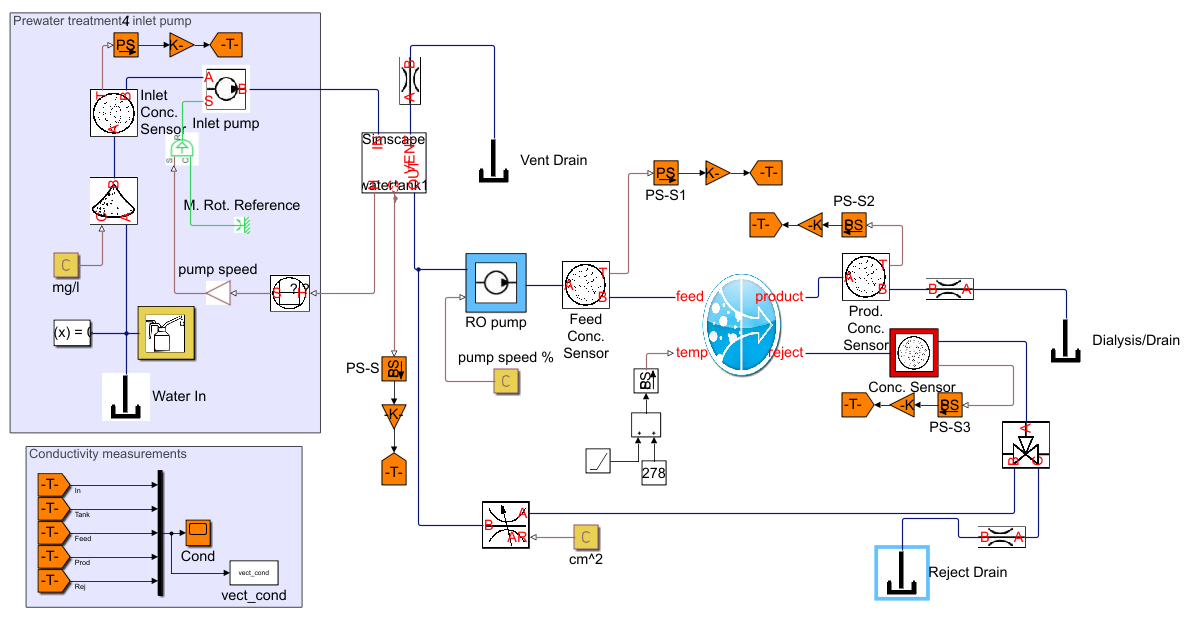
\includegraphics[width=\textwidth]{simscape_fc1.PNG}
\caption{Model made in Matlab tool Simscape}
\end{figure}


\subsection{Temperature}
In figure \ref{fig:temp} the simulated temperature, 278-316 K is shown. All plots \ref{fig:msaltf} - \ref{fig:conden} shows the behaviour over a simulated time of 2000 s and a temperature range of 278-316 K. Pump speed is kept constant. The temperature correction factor, TCF, in figure \ref{fig:tcf} is the temperature dependent parameter implemented in the simulated model to receive the differences of the behaviour of the membrane. At 298 K TCF is equal to 1. Below and above it is adjusted to compensate for the differences of the membrane behaviour. \\
\\
\begin{figure}[h]
  \centering
  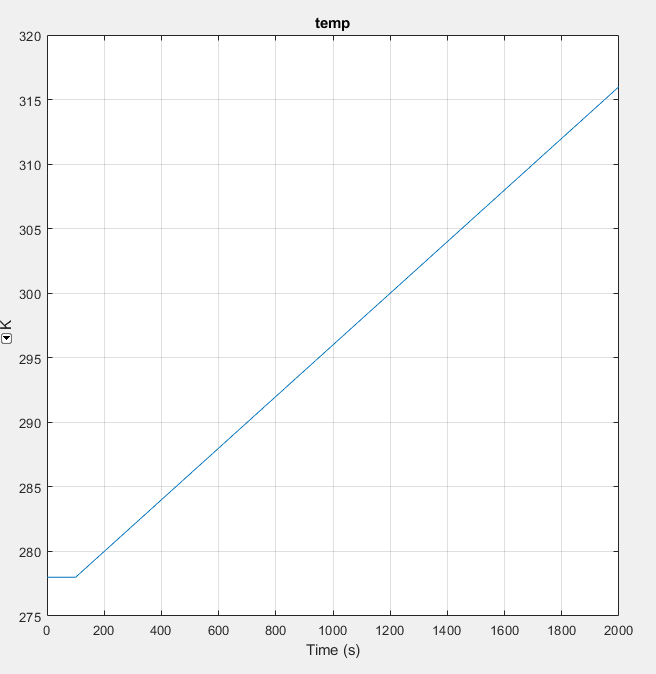
\includegraphics[width=0.5\linewidth]{temp.PNG}
  \caption{Temperature}
  \label{fig:temp}
\end{figure}
\begin{figure}[h]
\centering
    \centering
    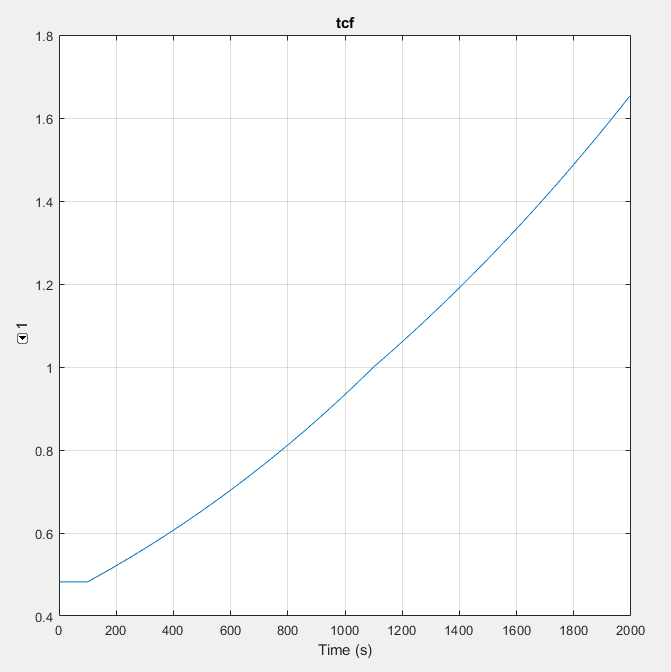
\includegraphics[width=0.5\textwidth]{tcf.PNG}
    \caption{Temperature correction factor}
    \label{fig:tcf}
\end{figure}

\subsection{Salt koncentration}

In figure \ref{fig:msaltf} the salt koncentration in kg/s on feed side of the membrane is shown. The concentration increases over the simulated time and change in temperature. \\
In figure \ref{fig:msaltp} the salt koncentration on product side is shown. Due to the mass balance equation in XXXX the sign is negative, and the koncentration increases with temperature.\\
In figure \ref{fig:msaltr} the salt koncentration on reject side is shown. It increases a little with temperature (negative sign due to the mass balance equations).\\
The product salt koncentration increases with from a value of  0.8 - 0.96 kg/s. The product water koncentration increases from (-) 0.2 - 1.8 kg/s. The reject salt koncentration increases from (-) 0.8 - 0.96 kg/s.\\
\\
\begin{figure}[h]
\centering
    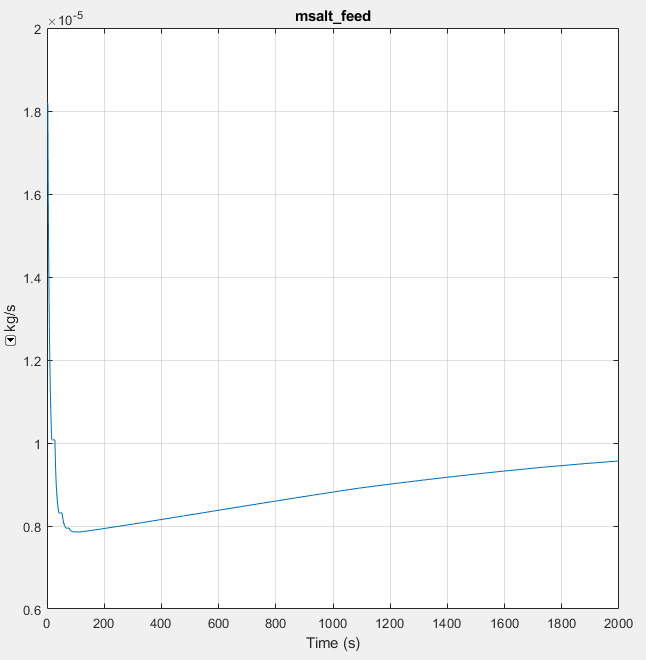
\includegraphics[width=0.5\textwidth]{msalt_feed.PNG}
    \caption{Salt concentration feedwater}
    \label{fig:msaltf}
\end{figure}
\begin{figure}[h]
\centering
  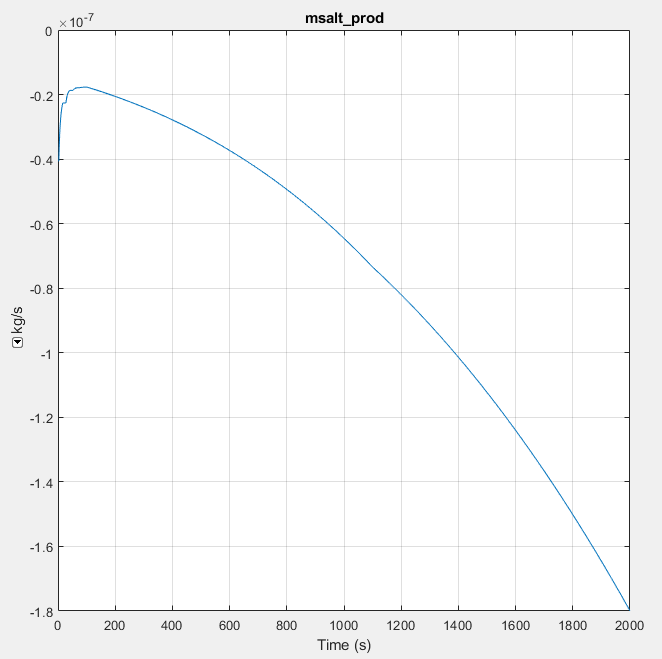
\includegraphics[width=0.5\linewidth]{msalt_prod.PNG}
  \caption{Salt concentration productwater}
  \label{fig:msaltp}
\end{figure}
\begin{figure}[h]
  \centering
  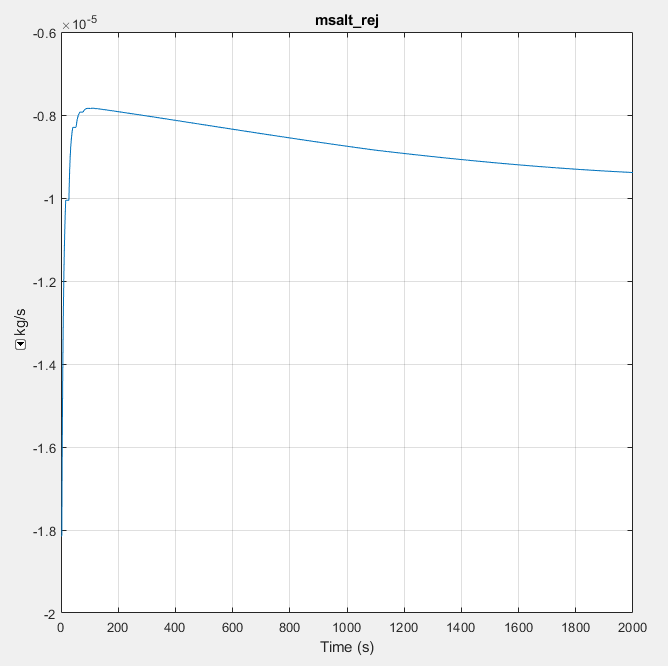
\includegraphics[width=0.5\linewidth]{msalt_rej.PNG}
  \caption{Salt concentration reject water}
  \label{fig:msaltr}
\end{figure}
Figure \ref{fig:qf} - \ref{fig:qrej} shows the flow in the three nodes; feed, product and reject. The mass balance equation in XXXX gives negative sign on reject and product side. The feed water flow increases negligible from 8.441-8.444 l/min. Product water flow increases from (-) 0.62-1.42 l/min. Reject water flow decreases from (-) 7.82-7.2 l/min. \\
\\

\subsection{Flow}
\begin{figure}[h]
  \centering
  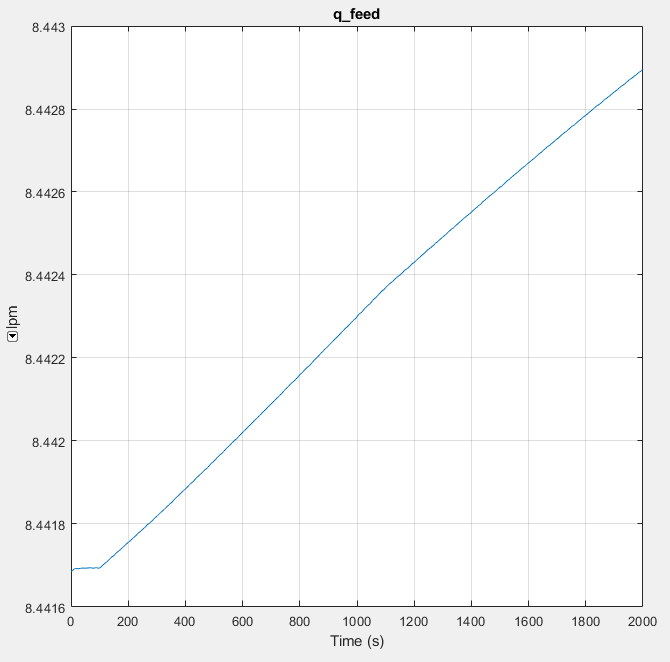
\includegraphics[width=0.5\linewidth]{q_feed.PNG}
  \caption{Flow feed side}
  \label{fig:qf}
\end{figure}
\begin{figure}[h]
  \centering
  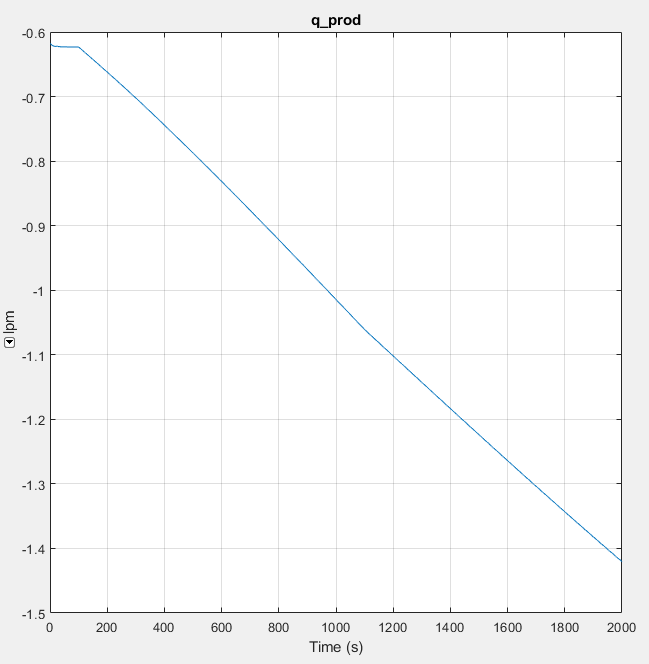
\includegraphics[width=0.5\linewidth]{q_prod.PNG}
  \caption{Flow product side}
  \label{fig:qp}
\end{figure}
\begin{figure}[h]
  \centering
  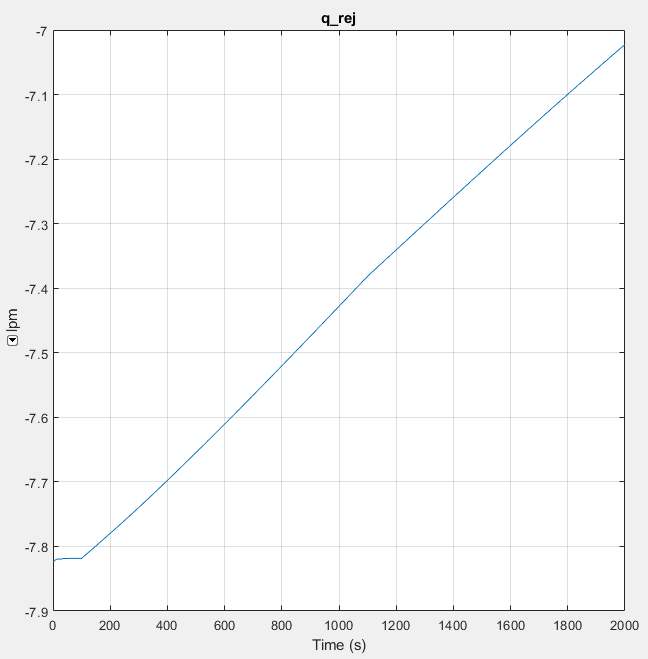
\includegraphics[width=0.5\linewidth]{q_rej.PNG}
  \caption{Flow reject side}
  \label{fig:qrej}
\end{figure}

\subsection{Pressure}
Figure \ref{fig:deltap} shows pressure difference from feed side to product side. The pressure decreases from (-) 11.5-7.7 bar when temperature changes from 278-316 K. \\
\\
\begin{figure}[h]
  \centering
  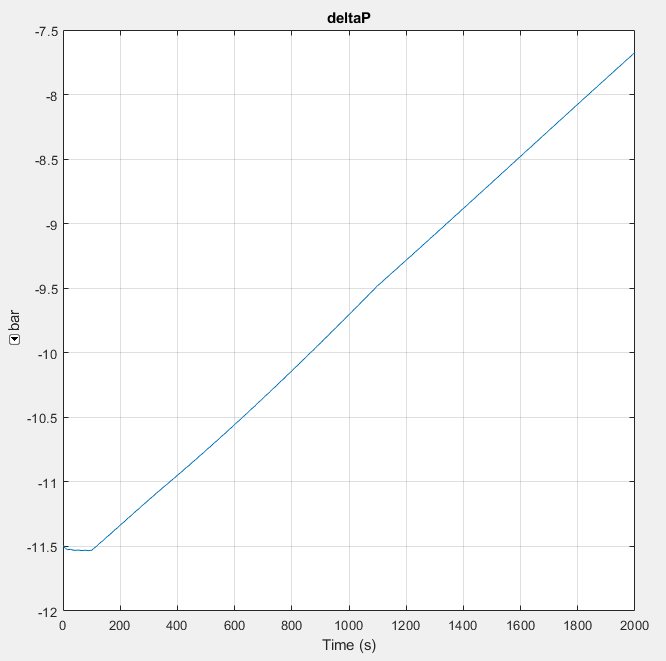
\includegraphics[width=0.5\linewidth]{deltap.PNG}
  \caption{Pressure drop feed side to product side}
  \label{fig:deltap}
\end{figure}

\subsection{Conductivity}
Figure \ref{fig:conden} displays the conductivity in feed, product and reject side. The conductivity in all nodes increases when temperature increases.\\
\\
\begin{figure}[h]
  \label{fig:conden}
  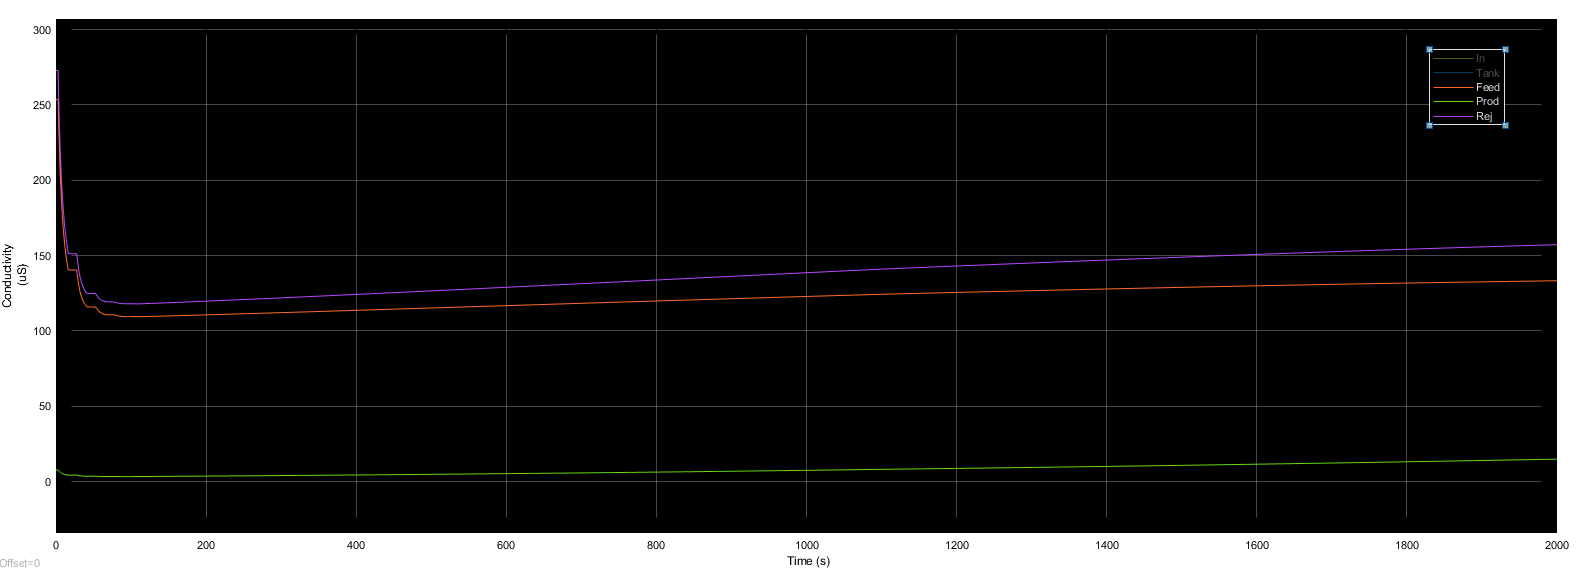
\includegraphics[width=1.1\linewidth]{cond.PNG}
  \caption{Conductivity in feed, reject and product side}
\end{figure}

\newpage


\section{Flowchart investigation}
By changing the flow path in the test setup both the one pump system and two pump system could be investigated and their performance could be compared. Both Systems were considered fulfilling most of the requirements, section \ref{framing}, for an updated version. \\

One pump system, figure \ref{fig:FlowCInves1}, The one pump system was designed to use both a tank and the recirculation loop as a water source and to create pressure by generating a large flow over the membrane and recirculation restrictor. \\


Two pump system, figure \ref{fig:Sys2}, In the two pump system the water path was modified so that the feed pump only used a tank as a source and pressureized the entire recirculation loop. The recirculation pump was used to recirculate the already\\ pressurized water within the recirculation loop.\\


An overview of the systems can be seen below.\\
\begin{figure}[h]
\centering
\begin{minipage}{.5\textwidth}
    \centering
    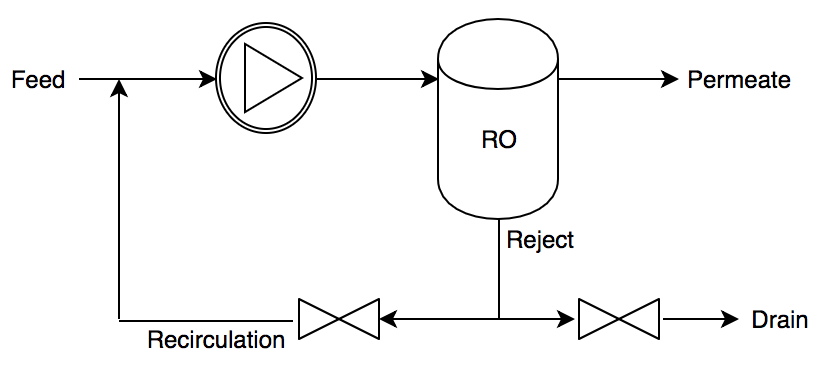
\includegraphics[width=0.8\textwidth]{Sys1}
    \caption{One pump system}
    \label{fig:System1}
\end{minipage}%
\begin{minipage}{.5\textwidth}
  \centering
  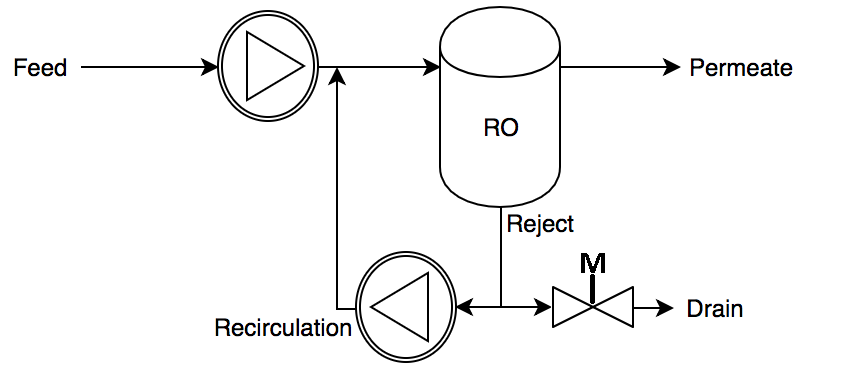
\includegraphics[width=.8\linewidth]{Sys2}
  \caption{Two pump system}
  \label{fig:System2}
\end{minipage}
\end{figure}

\newpage

\section{Mapping}
The mapping of the pumps RPM and flowrate can be seen in \ref{fig:RPM} and \ref{fig:Flowrate}.
\begin{figure}[h]
    \centering
    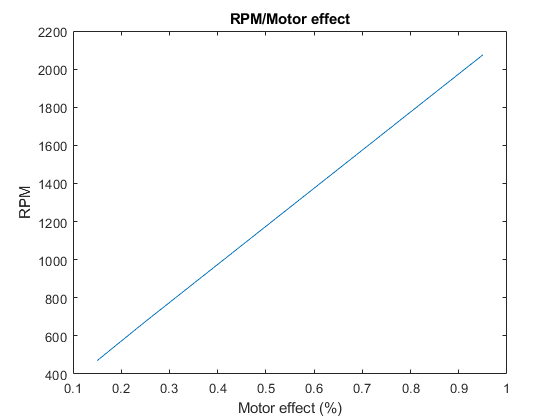
\includegraphics[width=0.7\textwidth]{RPM.png}
    \caption{RPM of the Pumps at different control signals/duty cycles}
    \label{fig:RPM}
\end{figure}


\begin{figure}[h]
    \centering
    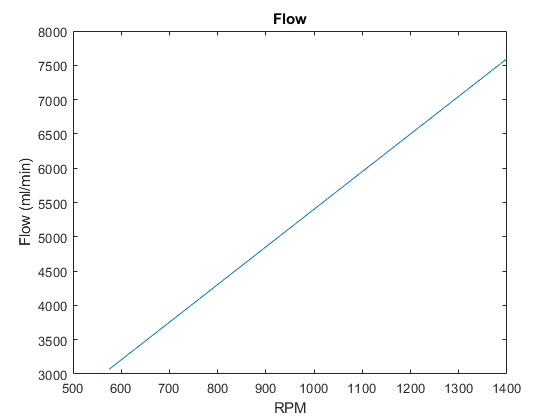
\includegraphics[width=0.7\textwidth]{Flow.png}
    \caption{Flow rate at different control signals/duty cycles}
    \label{fig:Flowrate}
\end{figure}

\section{Implementation Test Rig}


\subsection{Connections}
In Figure (\ref{fig:PressConn}-\ref{fig:PumpConn}) all connections in the test rig is displayed. The whole rig can be seen in \ref{fig:Rig1} and \ref{fig:Rig2}

\begin{figure}[h]
    \centering
    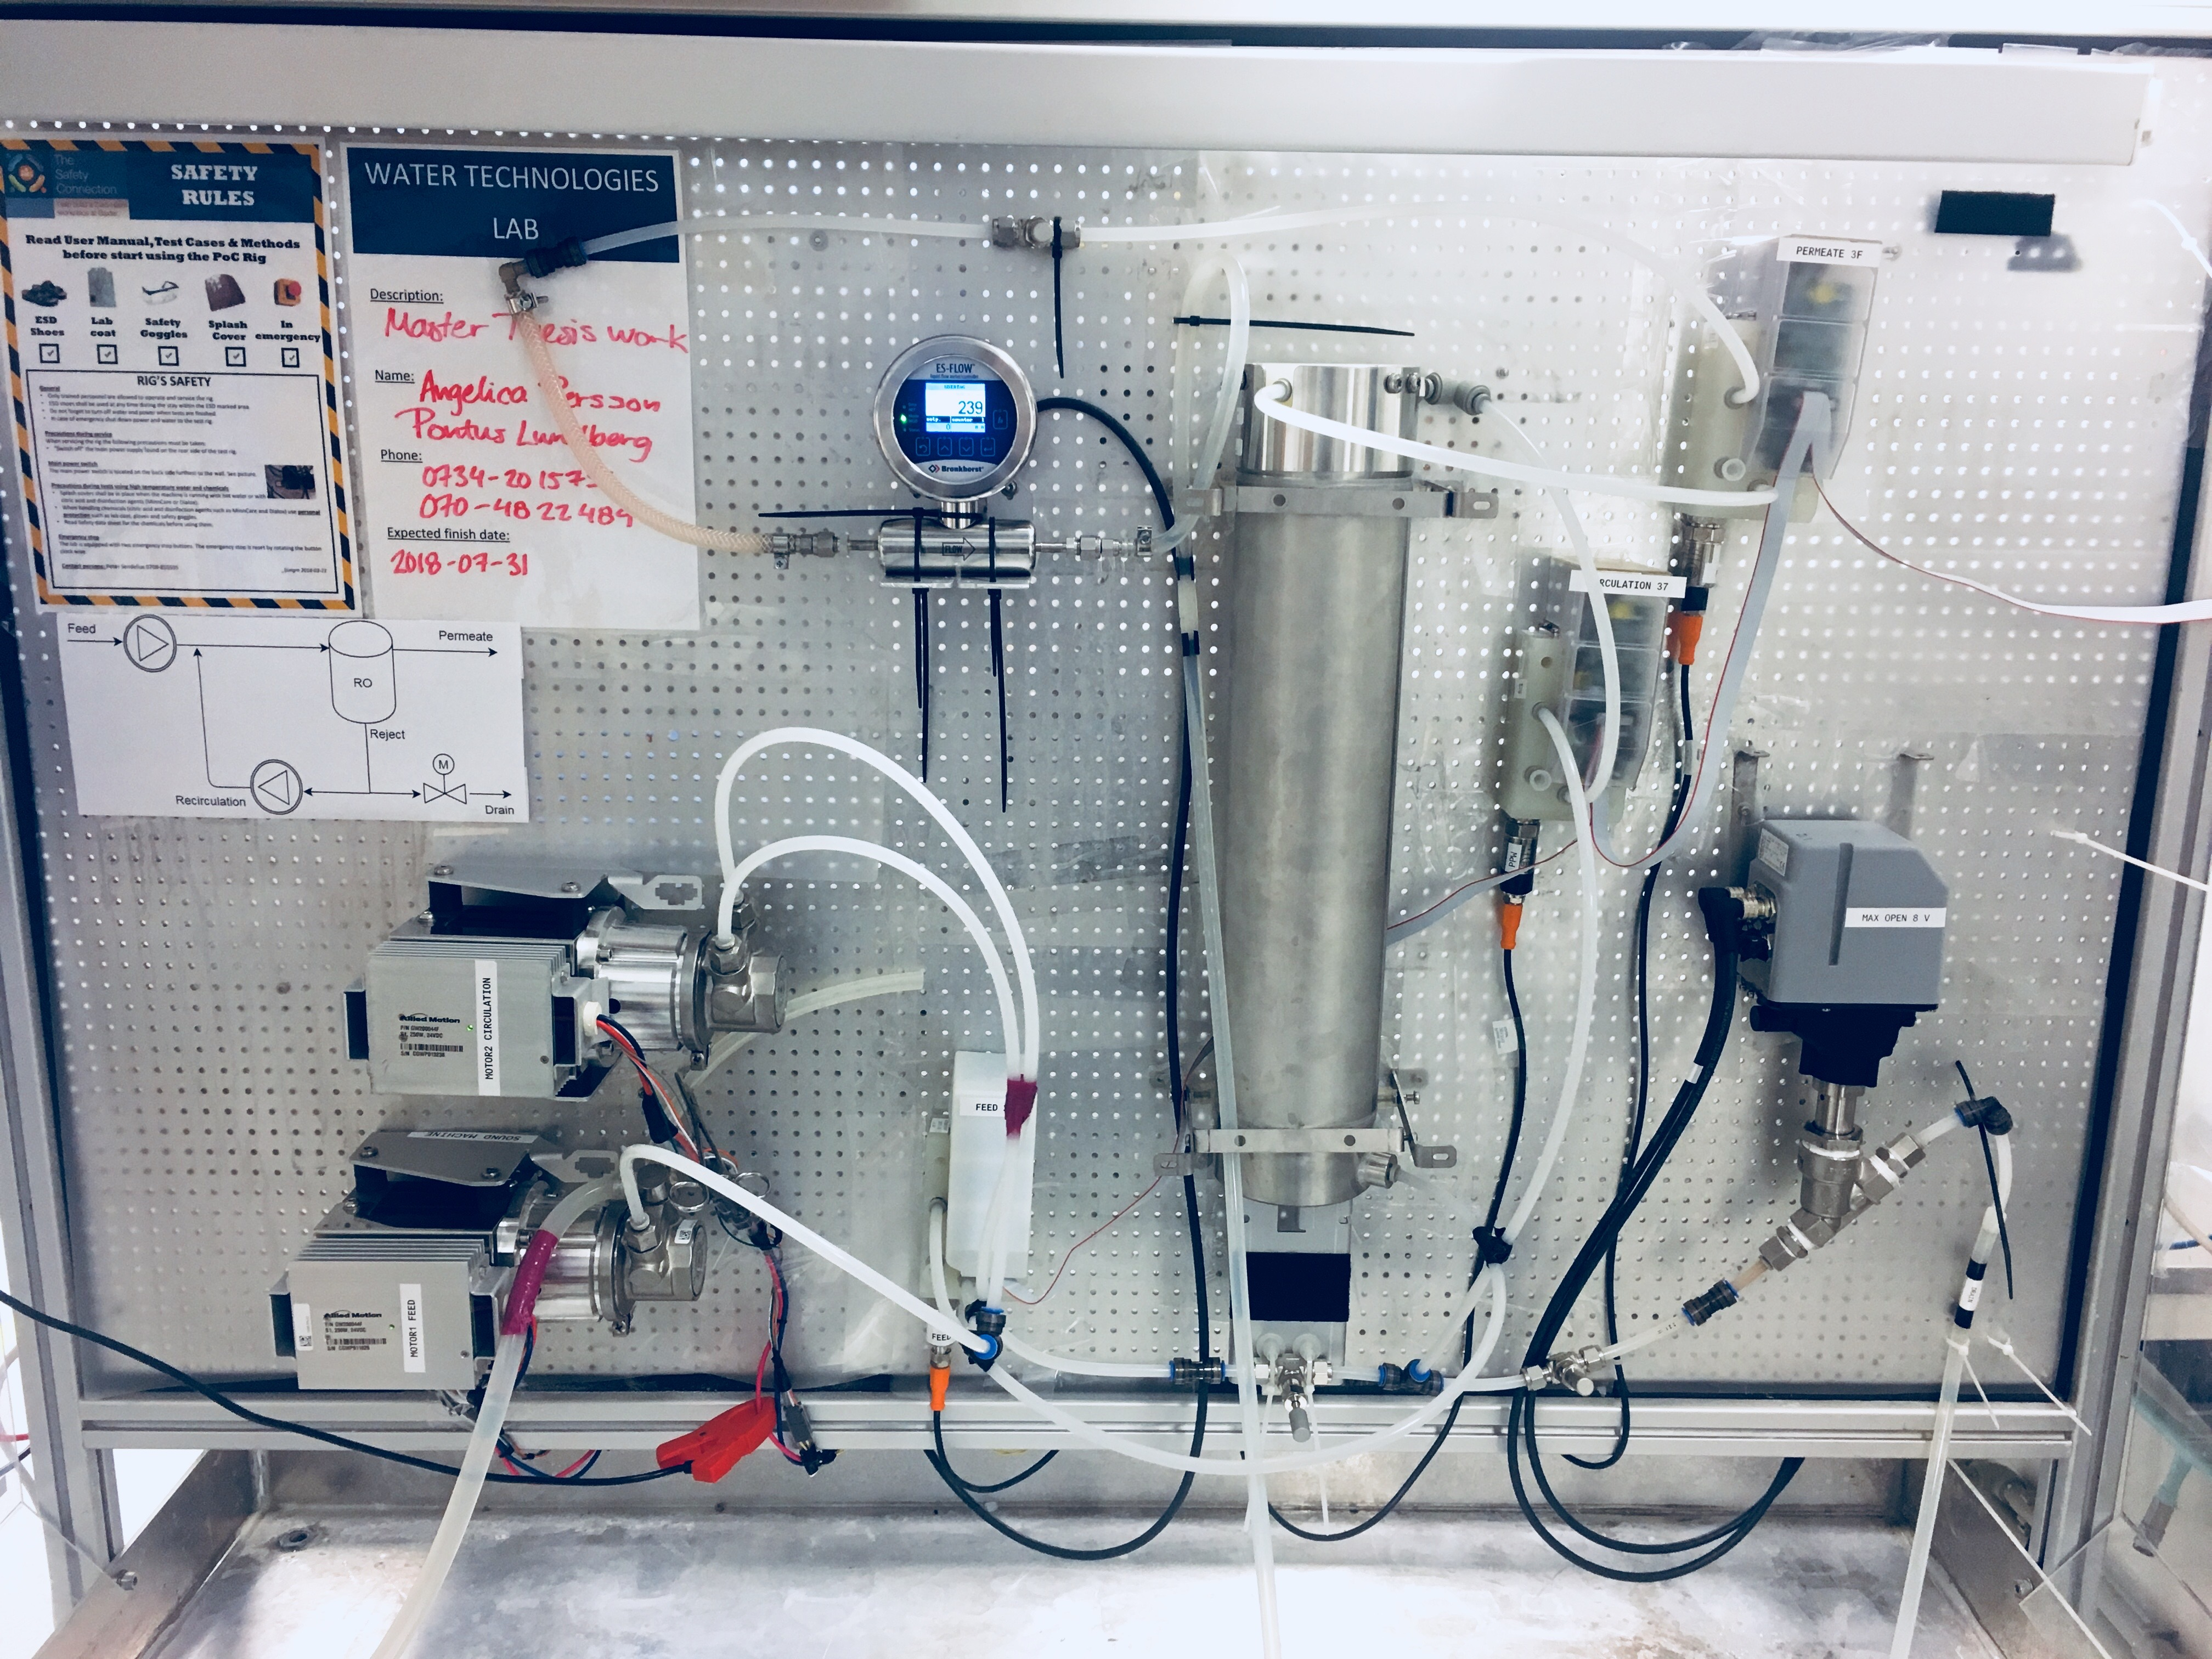
\includegraphics[width=0.5\textwidth]{Rig1}
    \caption{The rig built at Baxter Lund AB, with RO-membrane, pumps, pipes, flowmeter, measuremet sensors and valves}
    \label{fig:Rig1}
\end{figure}

\begin{figure}[h]
    \centering
    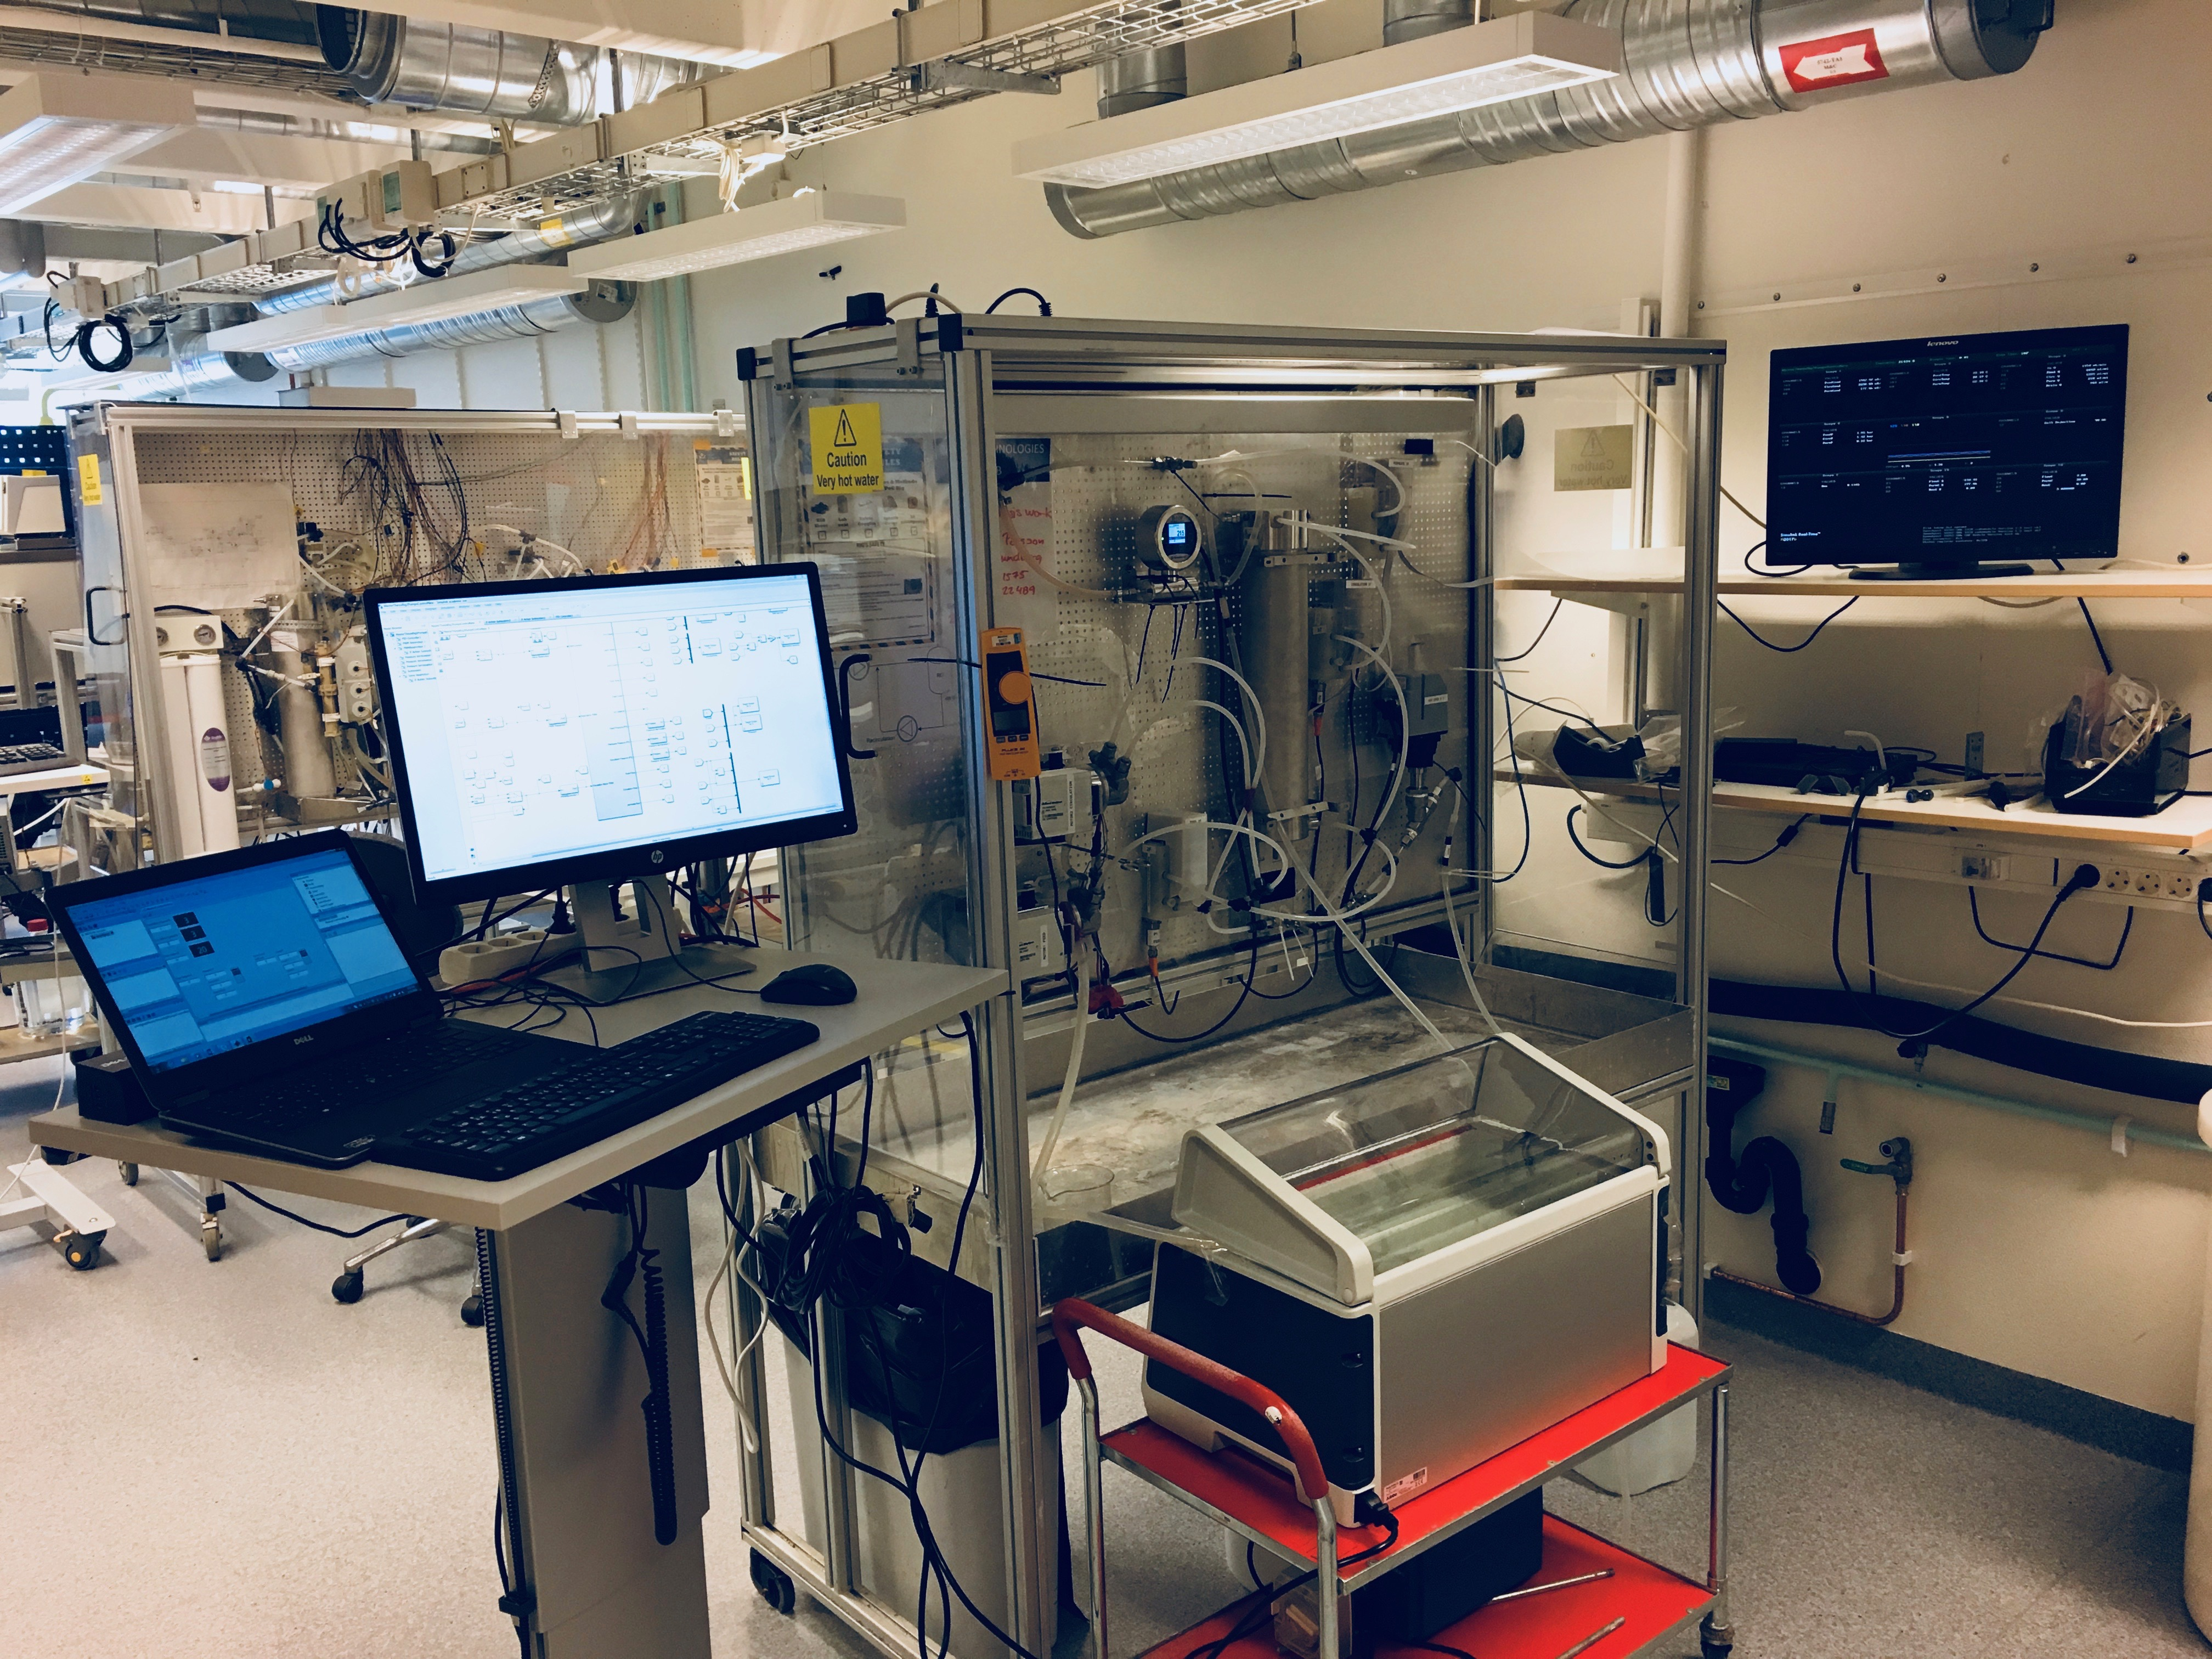
\includegraphics[width=0.5\textwidth]{Rig2}
    \caption{The full setup built at Baxter Lund AB, with simulink implementation, GUI, display and water bath}
    \label{fig:Rig2}
\end{figure}


\begin{figure}[h]
    \centering
    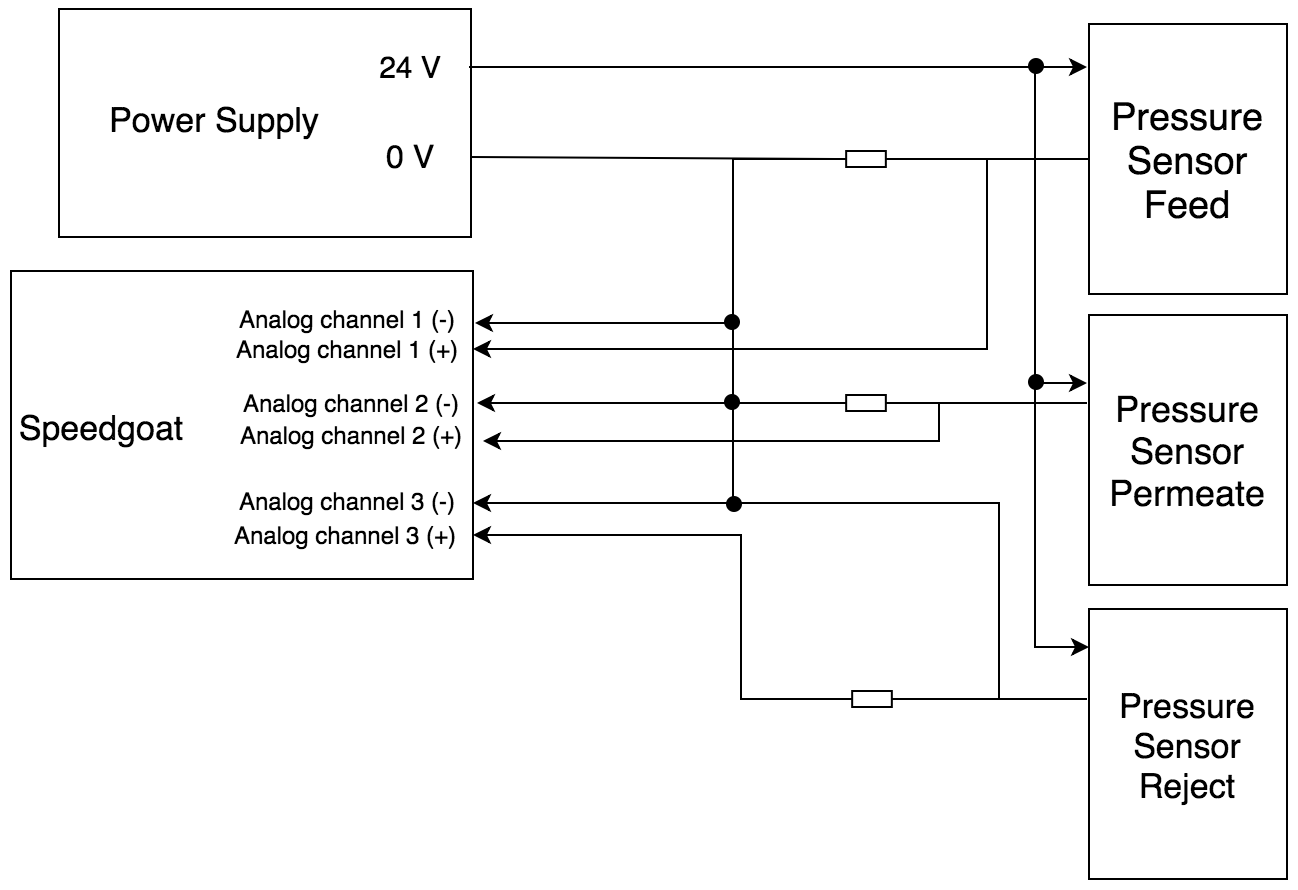
\includegraphics[width=0.6\textwidth]{PressConn}
    \caption{Connections Pressure sensors}
    \label{fig:PressConn}
\end{figure}

\newpage

\begin{figure}[h]
    \centering
    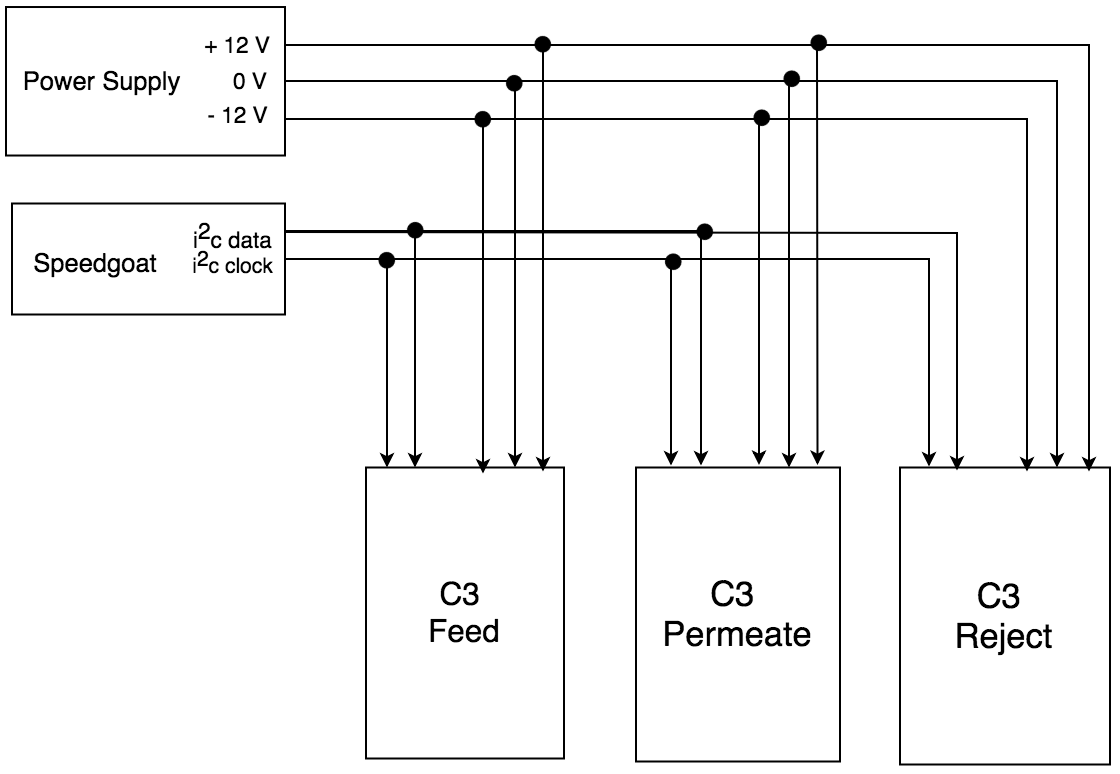
\includegraphics[width=0.6\textwidth]{C3Conn}
    \caption{Connections measurement blocks, C3}
    \label{fig:C3Conn}
\end{figure}

\begin{figure}[h]
    \centering
    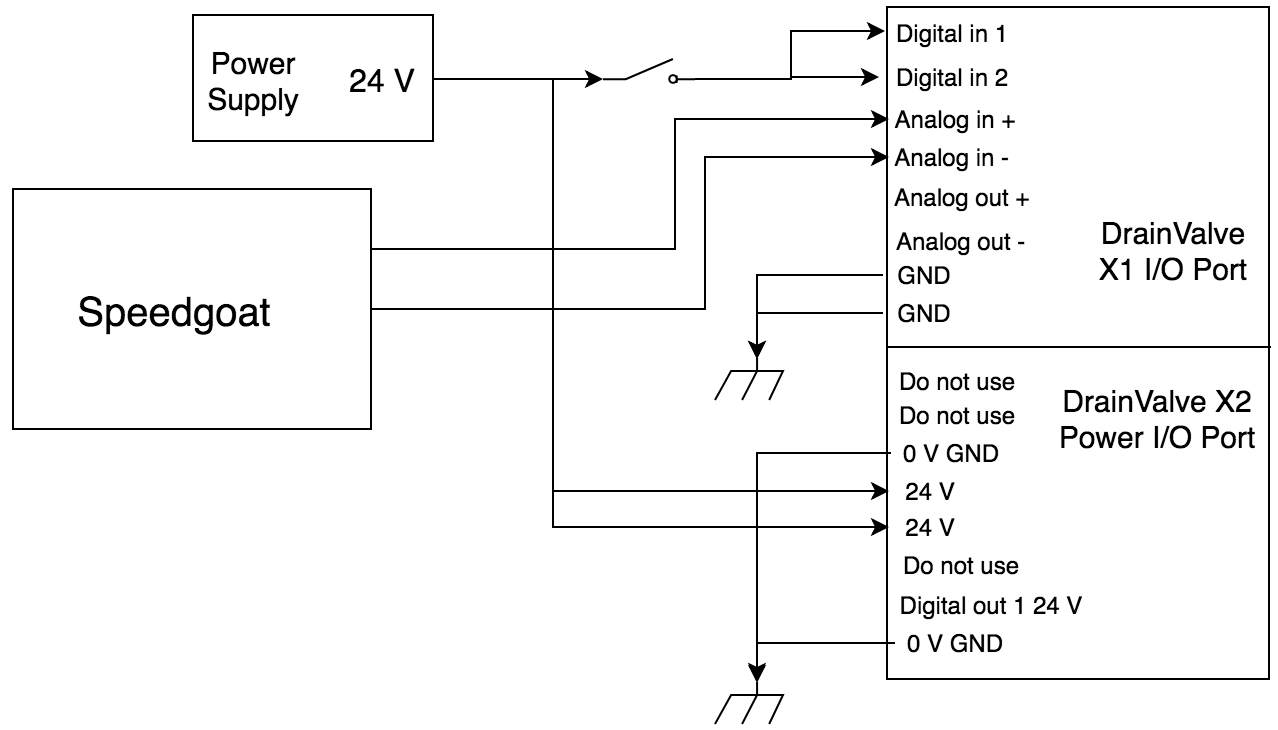
\includegraphics[width=0.6\textwidth]{ValveConn}
    \caption{Connections Drain Valve}
    \label{fig:ValveConn}
\end{figure}

\newpage

\begin{figure}[H]
    \centering
    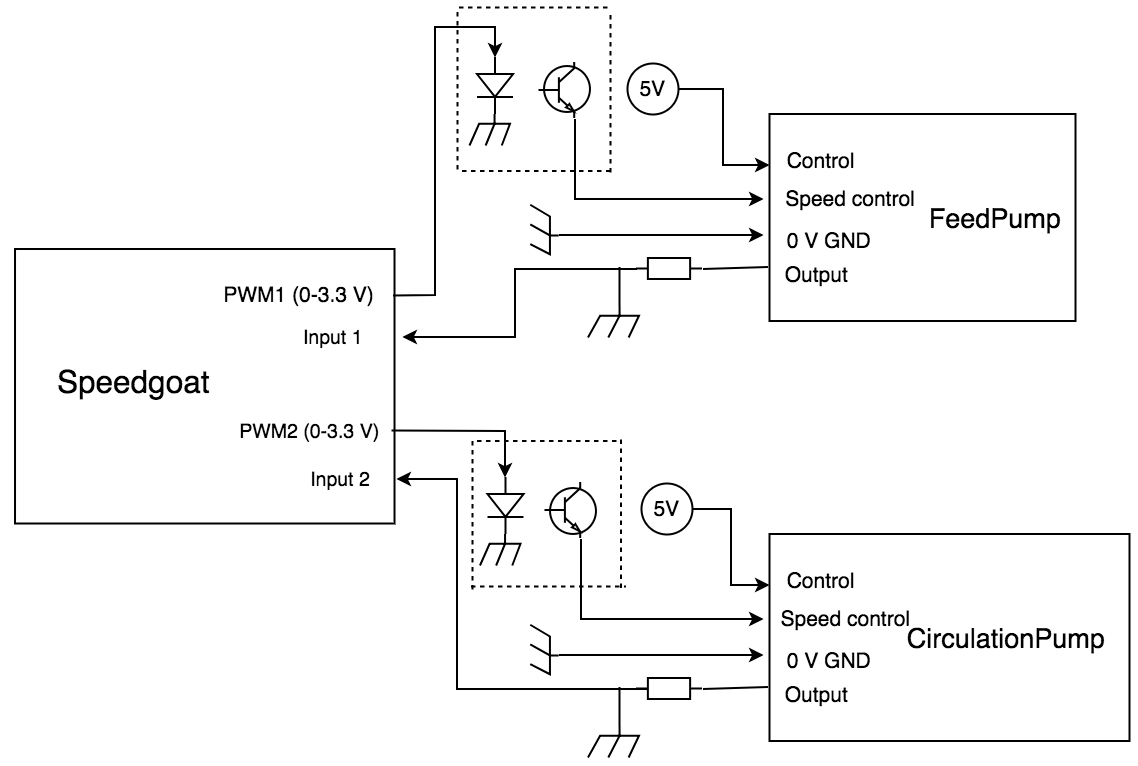
\includegraphics[width=0.6\textwidth]{PumpConn}
    \caption{Connections pumps}
    \label{fig:PumpConn}
\end{figure}
\begin{figure}[H]
    \centering
    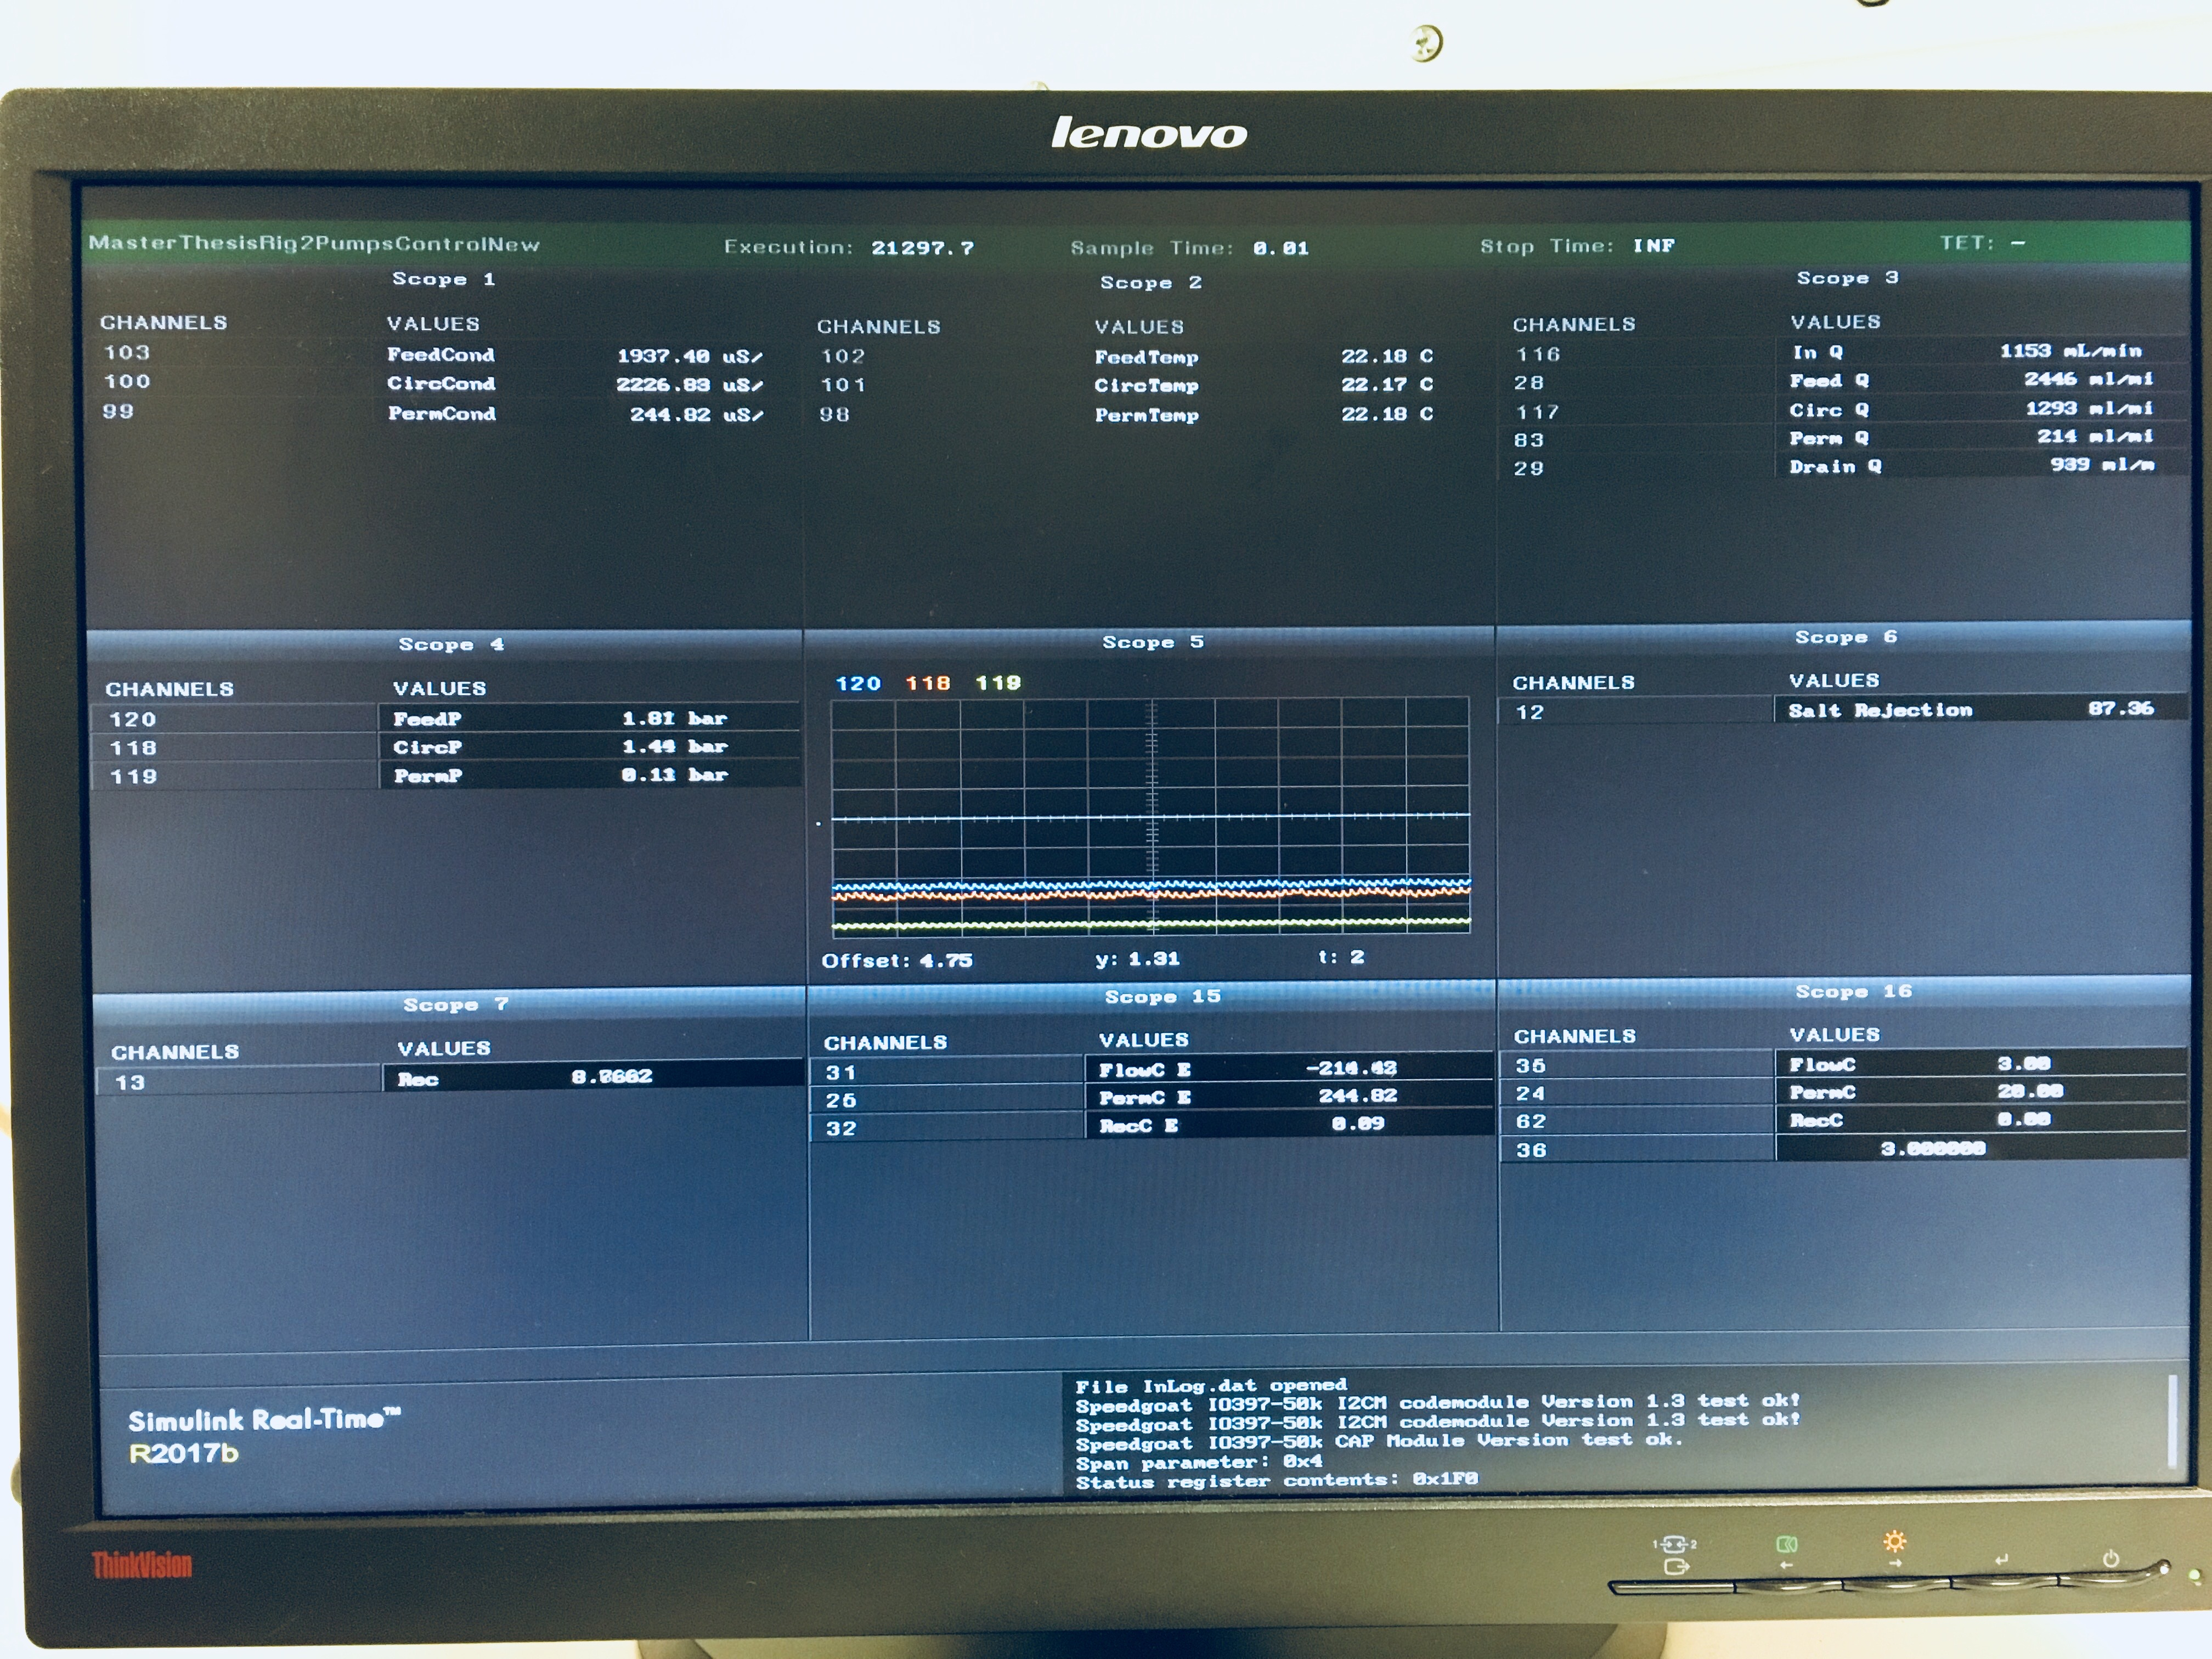
\includegraphics[width=0.6\textwidth]{Display}
    \caption{The Display with all key values, read from sensors in the rig}
    \label{fig:display}
\end{figure}
\begin{figure}[H]
    \centering
    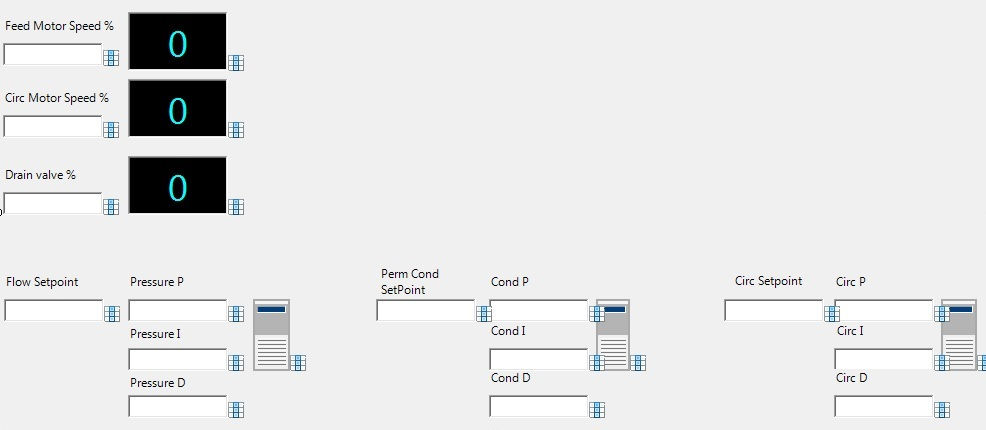
\includegraphics[width=0.6\textwidth]{GUI}
    \caption{The GUI implemented in Simulink and used to control the rig}
    \label{fig:gui}
\end{figure}


\newpage


\section{Investigation on membrane behaviour}

In order to compare the two systems and understand how the membrane performed in different working conditions both systems needed to be tested. The tests were conducted by controlling the temperature, pumps and the conductivity in the recirculation loop and log how the different conditions affected the system and the membrane. 

The tests were conducted by changing the temperature, recirculation conductivity and pump speed and meassure how the system behaved once it had reached steady state. The tests were divided into three test sequences. One test sequence was performed with room temperatured water (19 C), one with water heated to 30 C and in the last test sequence the water was heated to 40 C. Every test sequence included data from 8 steady state points with different settings on feed conductivity and pump speed. The test sequences are displayed in the table below. 

\begin{table}[h]
\centering
\begin{tabular}{|p{1.4cm}||p{2cm}|p{3.2cm}|p{1.8cm}|}
 \hline
 \textbf{Steady state }&Temperature&Feed Conductivity&Motor effect \\
 \hline
 1.1 & 18 $^\circ$C   & 280 \SI{}{\micro\siemens} & 60 \% \\
 1.2   &  18 $^\circ$C   & 500 \SI{}{\micro\siemens} & 60 \% \\
 1.3 &  18 $^\circ$C  &1000 \SI{}{\micro\siemens} & 60 \% \\
 1.4 &  18 $^\circ$C  &1000 \SI{}{\micro\siemens} & \textbf{80 \%} \\
 1.5 &18 $^\circ$C &2000 \SI{}{\micro\siemens}& 60 \%\\
 1.6 &18 $^\circ$C  &2000 \SI{}{\micro\siemens}& \textbf{80 \%}\\
 1.7   &18 $^\circ$C & 3000 \SI{}{\micro\siemens}&60 \% \\
 1.8   &18 $^\circ$C&3000 \SI{}{\micro\siemens}& \textbf{80 \%}\\
 \hline
 2.1 & 30 $^\circ$C & 280 \SI{}{\micro\siemens}&60 \%\\
 2.2 & 30 $^\circ$C &500 \SI{}{\micro\siemens}& 60 \%\\
 2.3 & 30 $^\circ$C&1000 \SI{}{\micro\siemens}& 60 \%\\
 2.4 & 30 $^\circ$C&1000 \SI{}{\micro\siemens}& \textbf{80 \%}\\
 2.5 & 30 $^\circ$C&2000 \SI{}{\micro\siemens}& 60 \%\\
 2.6 & 30 $^\circ$C&2000 \SI{}{\micro\siemens}& \textbf{80 \%}\\
 2.7 & 30 $^\circ$C& 3000 \SI{}{\micro\siemens}&60 \%\\
 2.8 & 30 $^\circ$C& 3000 \SI{}{\micro\siemens}&\textbf{80 \%}\\
 \hline 
 3.1 & 40 $^\circ$C& 280 \SI{}{\micro\siemens}& 60 \%\\
 3.2 & 40 $^\circ$C &500 \SI{}{\micro\siemens}& 60 \%\\
 3.3 & 40 $^\circ$C  & 1000 \SI{}{\micro\siemens}& 60 \%\\
 3.4 & 40 $^\circ$C  & 1000 \SI{}{\micro\siemens}& \textbf{80 \%}\\
 3.5 & 40 $^\circ$C&2000 \SI{}{\micro\siemens}& 60 \%\\
 3.6 & 40 $^\circ$C &2000 \SI{}{\micro\siemens}& \textbf{80 \%}\\
 3.7 & 40$^\circ$C &3000 \SI{}{\micro\siemens}& 60 \%\\
 3.8 & 40$^\circ$C &3000 \SI{}{\micro\siemens}& \textbf{80 \%}\\
\hline
\end{tabular}
\caption{Testcases}
    \label{tab:test cases} 
\end{table}


\newpage
\subsection{Current system, Test sequence 1, part 1}

The water in the tank was heated while the test was running. Because of this, the test was split up in two parts, first the motor was set to 60\% and steady state 1.1, 1.2, 1.3, 1.5 and 1.7 were investigated. In the part 2, the motor was set to 80 \% and steady state 1.4, 1.6 and 1.8 were investigated. 

\begin{figure}[h]
    \centering
    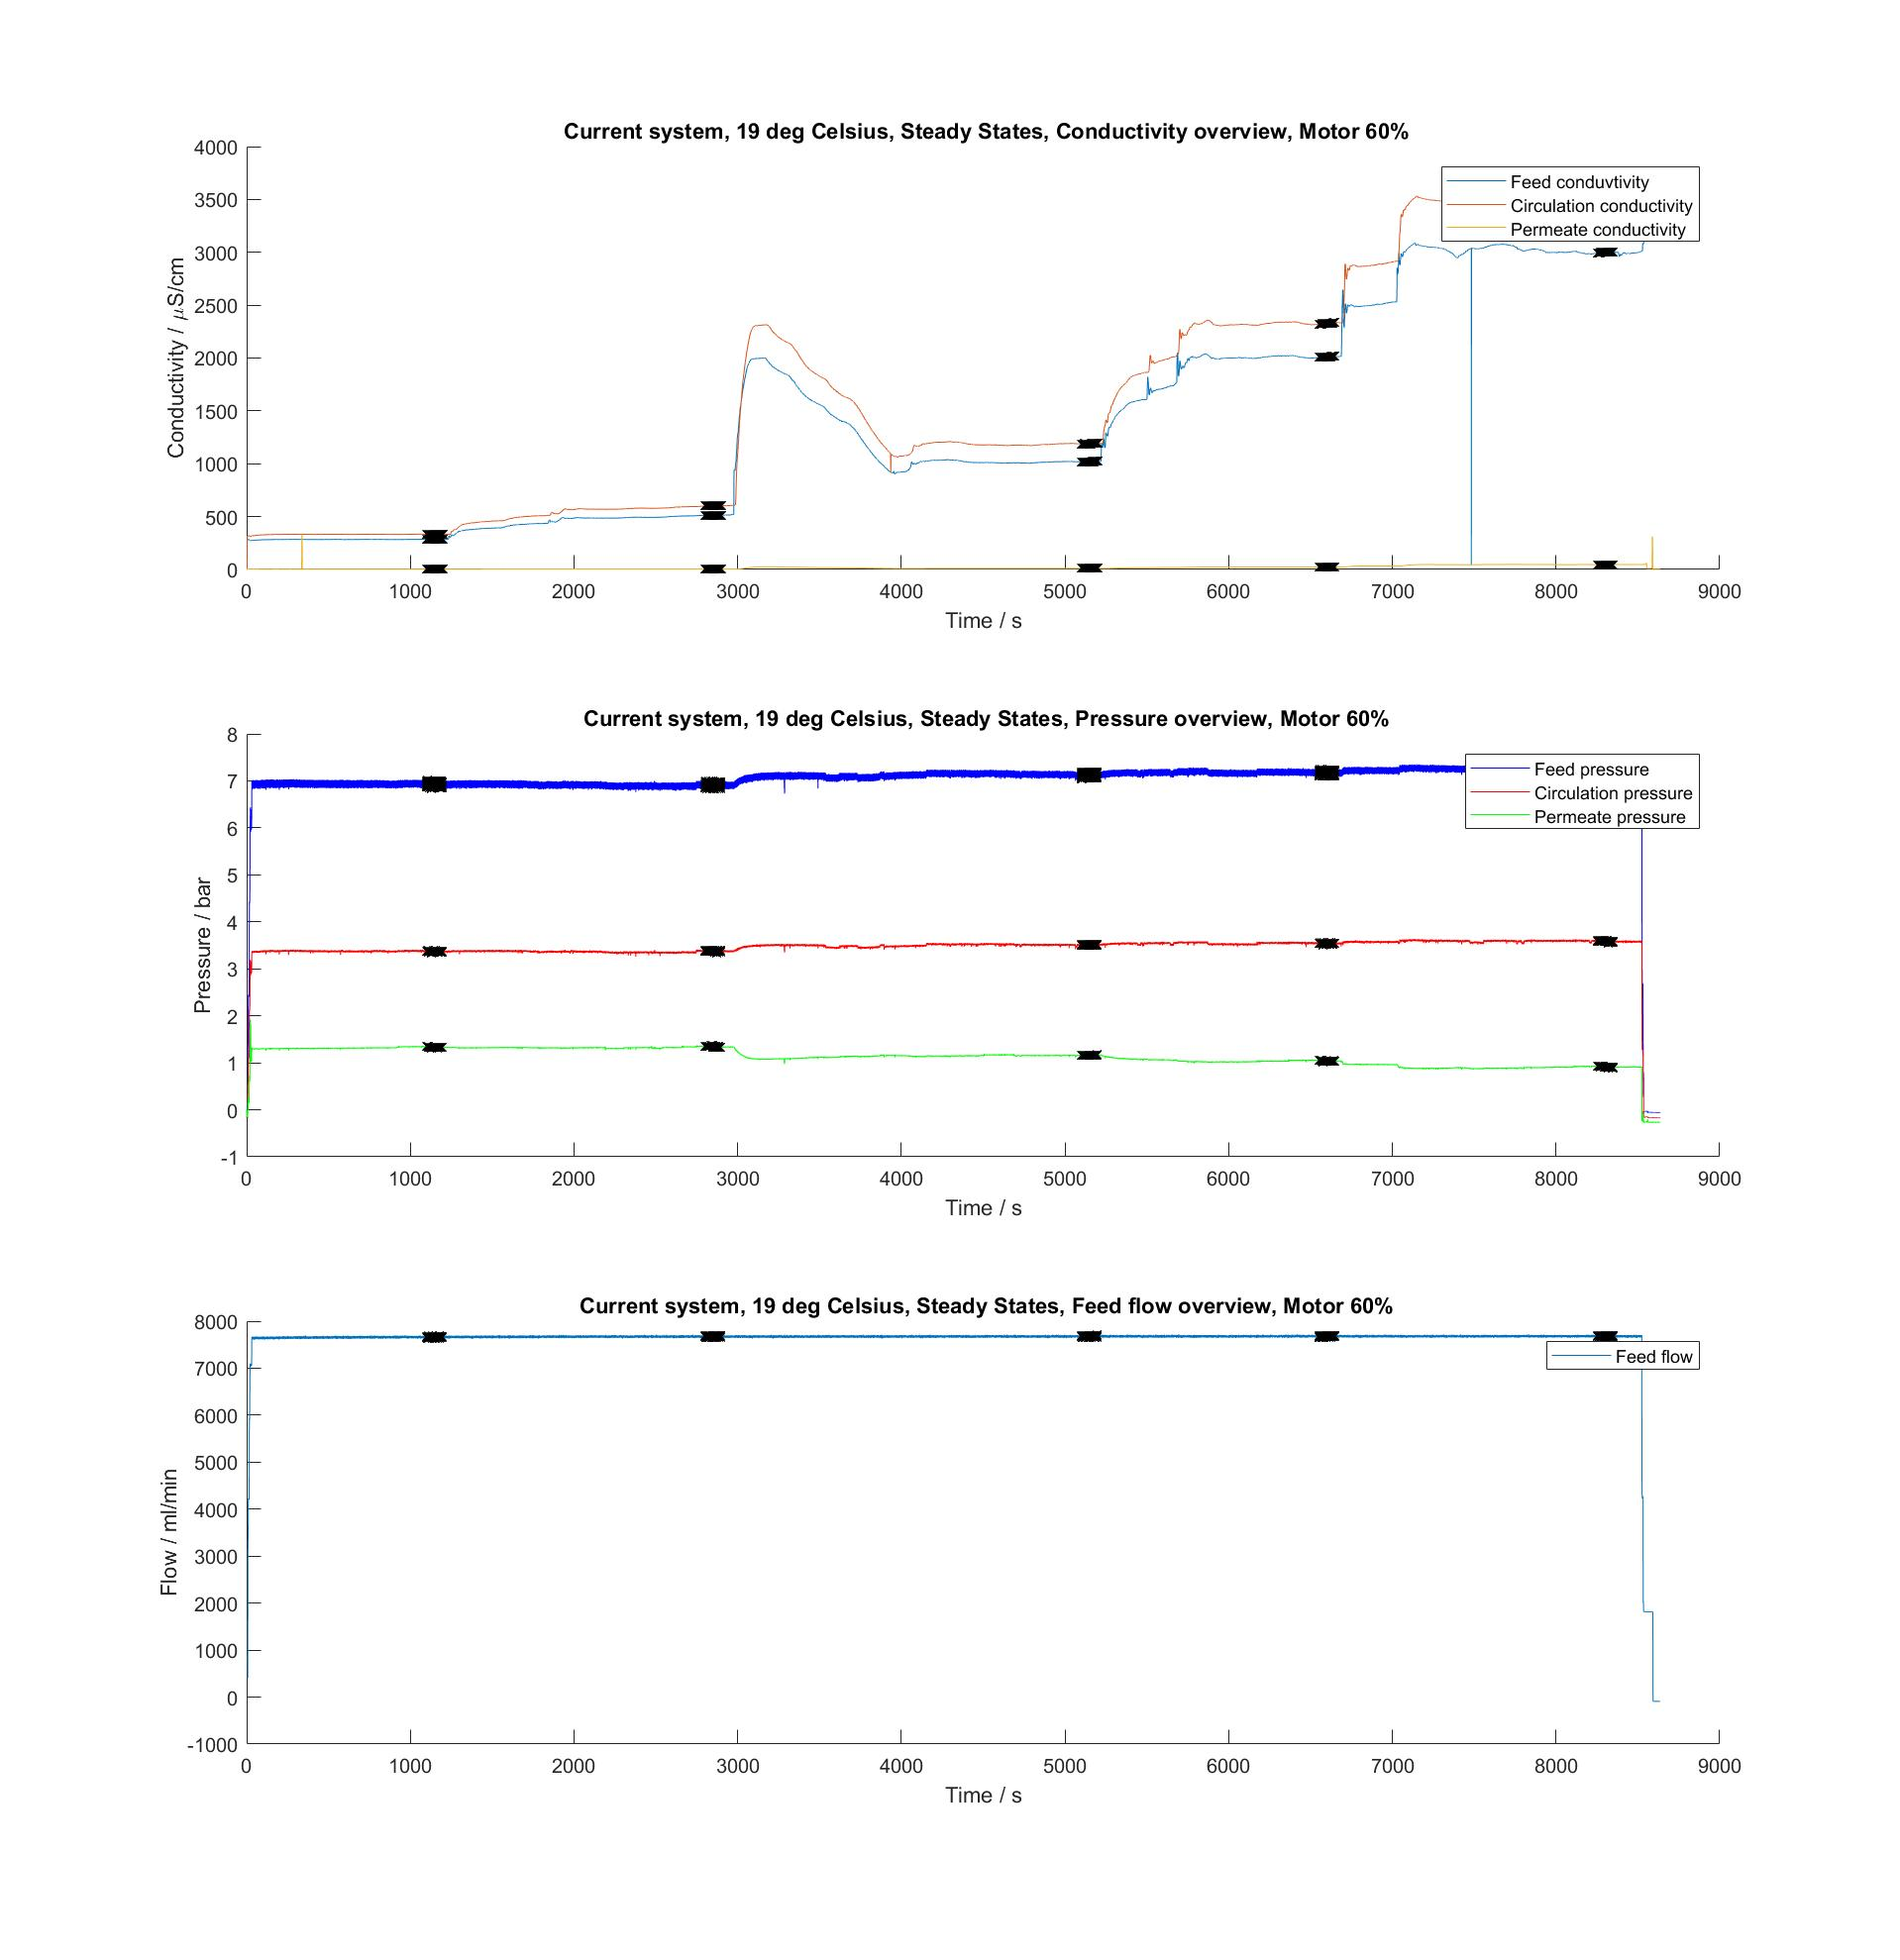
\includegraphics[width=1.1\textwidth]{overview20_60}
    \caption{Test 1, Current system, 18 degrees celsius. Steady states 1.1, 1.2, 1.3, 1.5 and 1.7 }
    \label{fig:PressConn}
\end{figure}

\newpage

\subsection{Current system, Test sequence 1, part 2}
  
\begin{figure}[H]
    \centering
    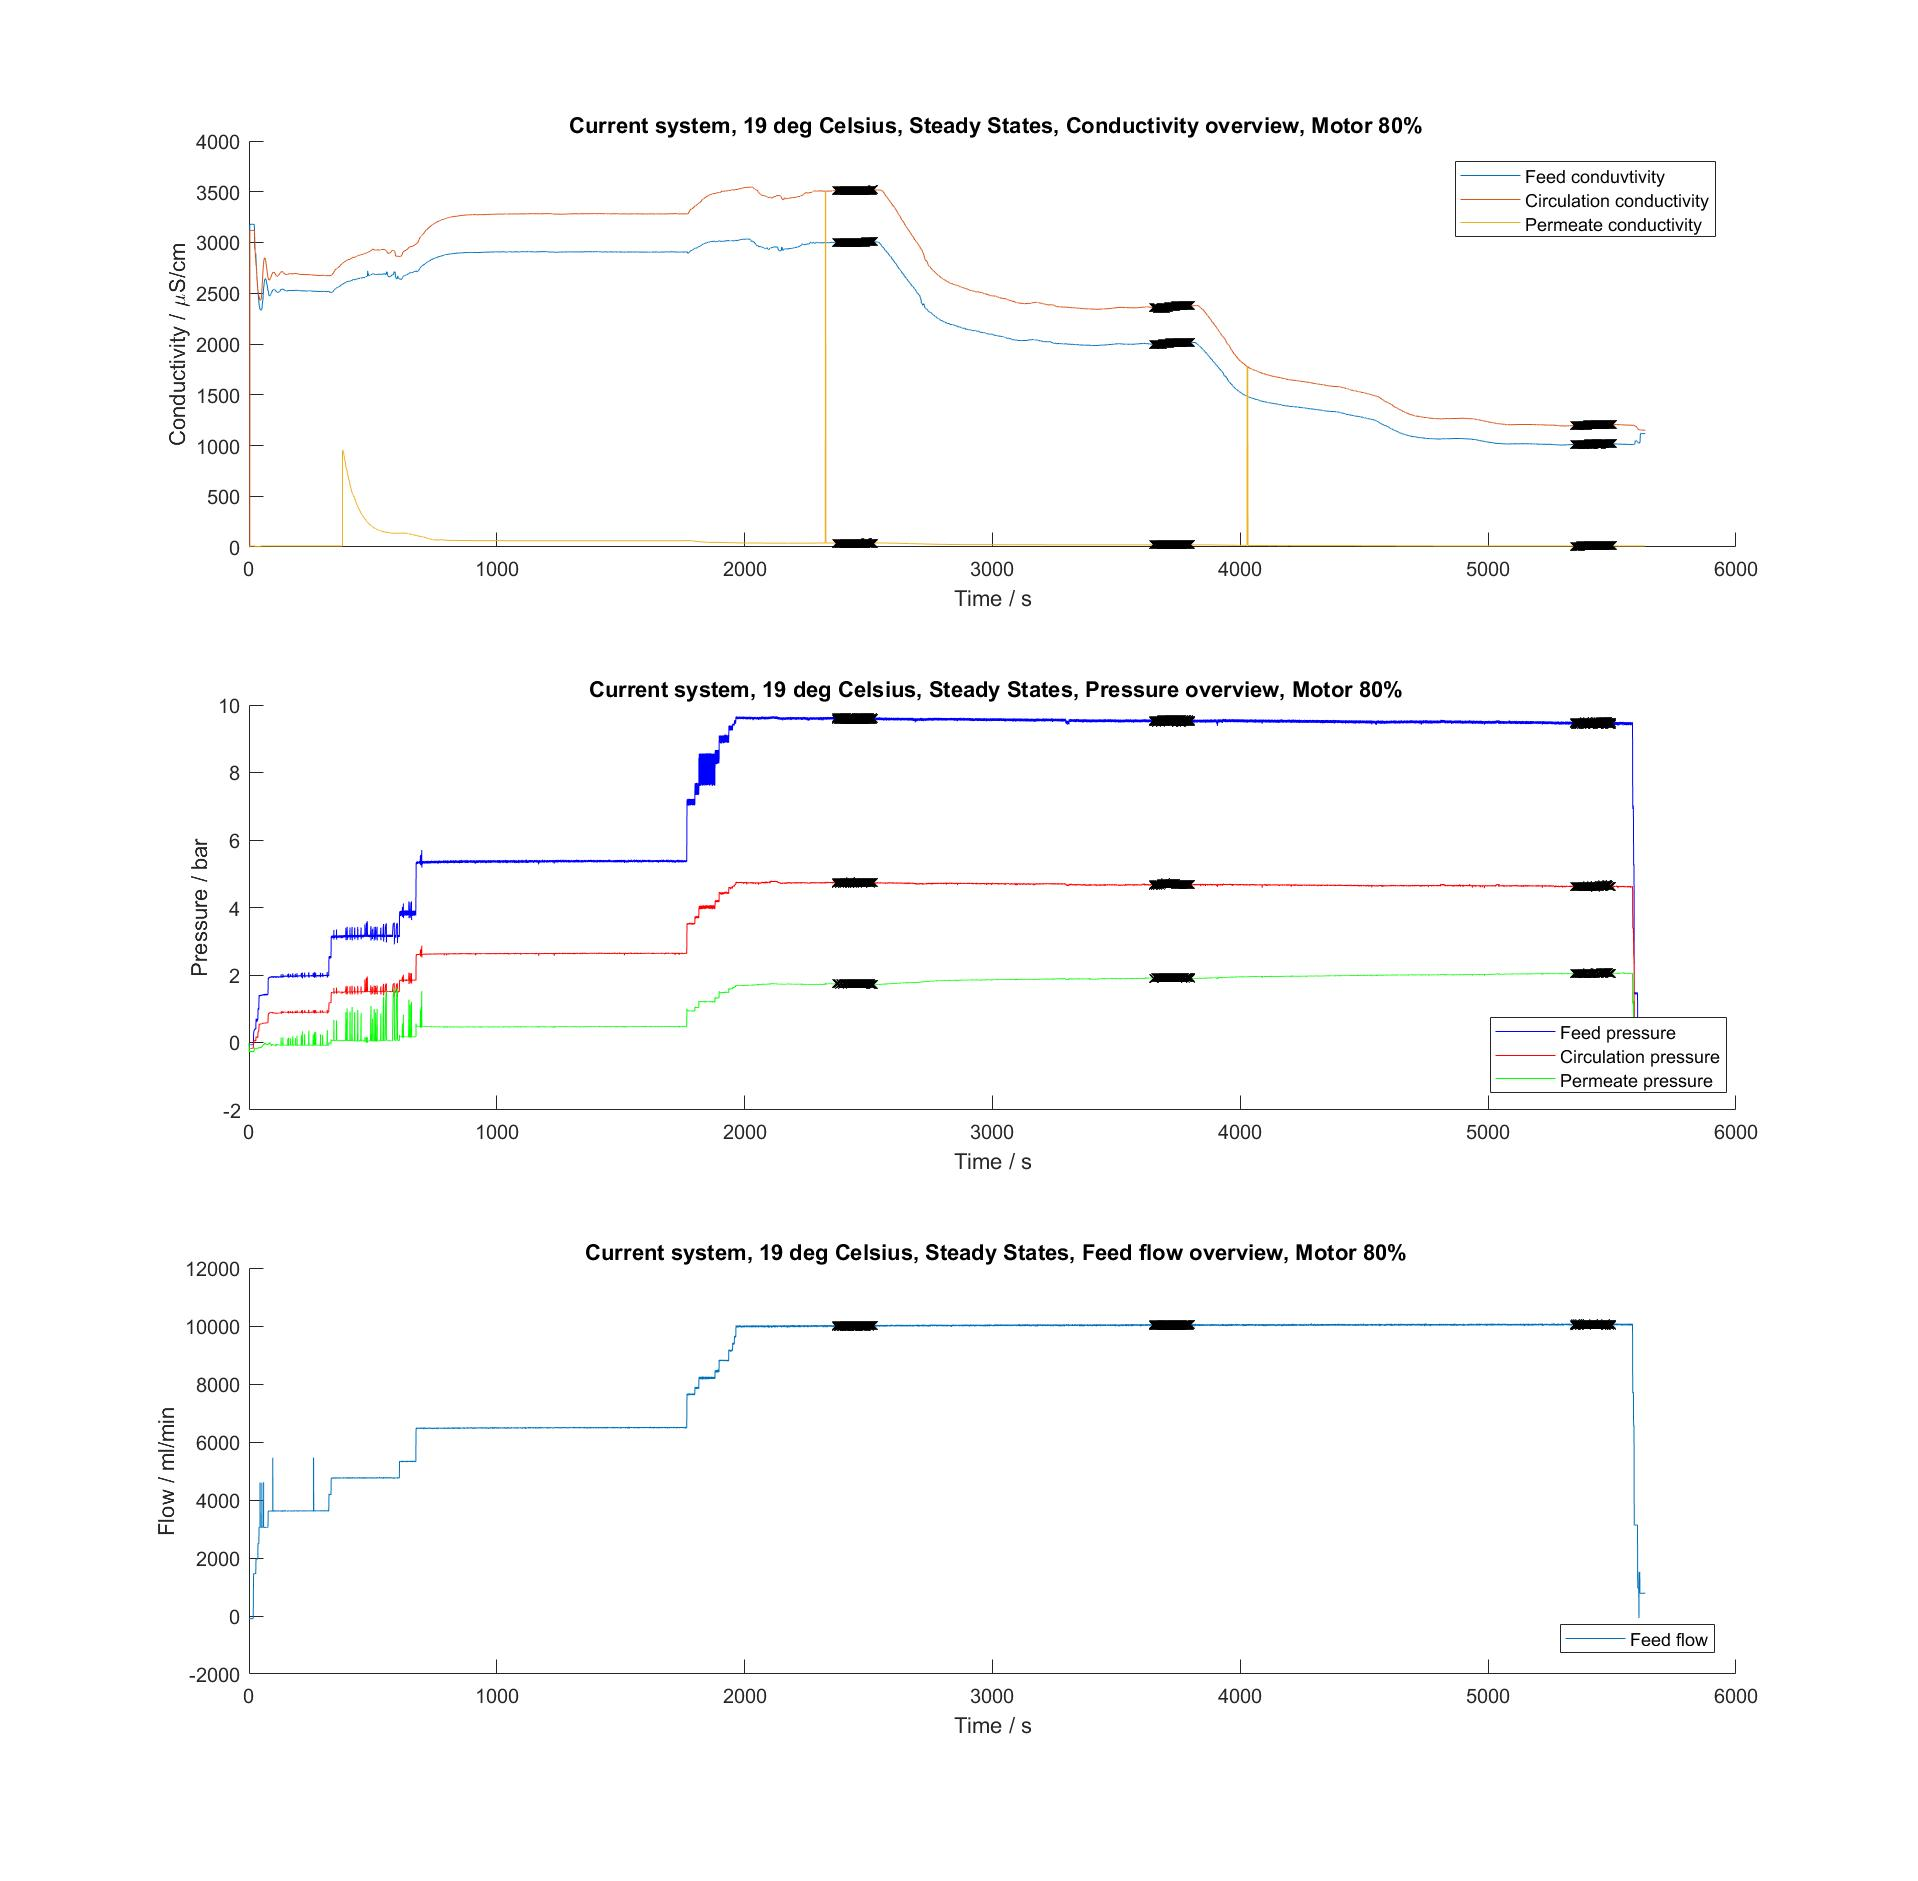
\includegraphics[width=1.1\textwidth]{overview20_80}
    \caption{Test 1, Current system, 18 degrees celsius. Steady states 1.4, 1.6 and 1.8}
    \label{fig:PressConn}
\end{figure}

\newpage

By post-proccesing the data from test one in Matlab it was possible to visually show how the system parameters were affected by the changed pump speed and feed conductivity. 


insert table, results on how the different graphs changed!!!

\begin{figure}[H]
    \centering
    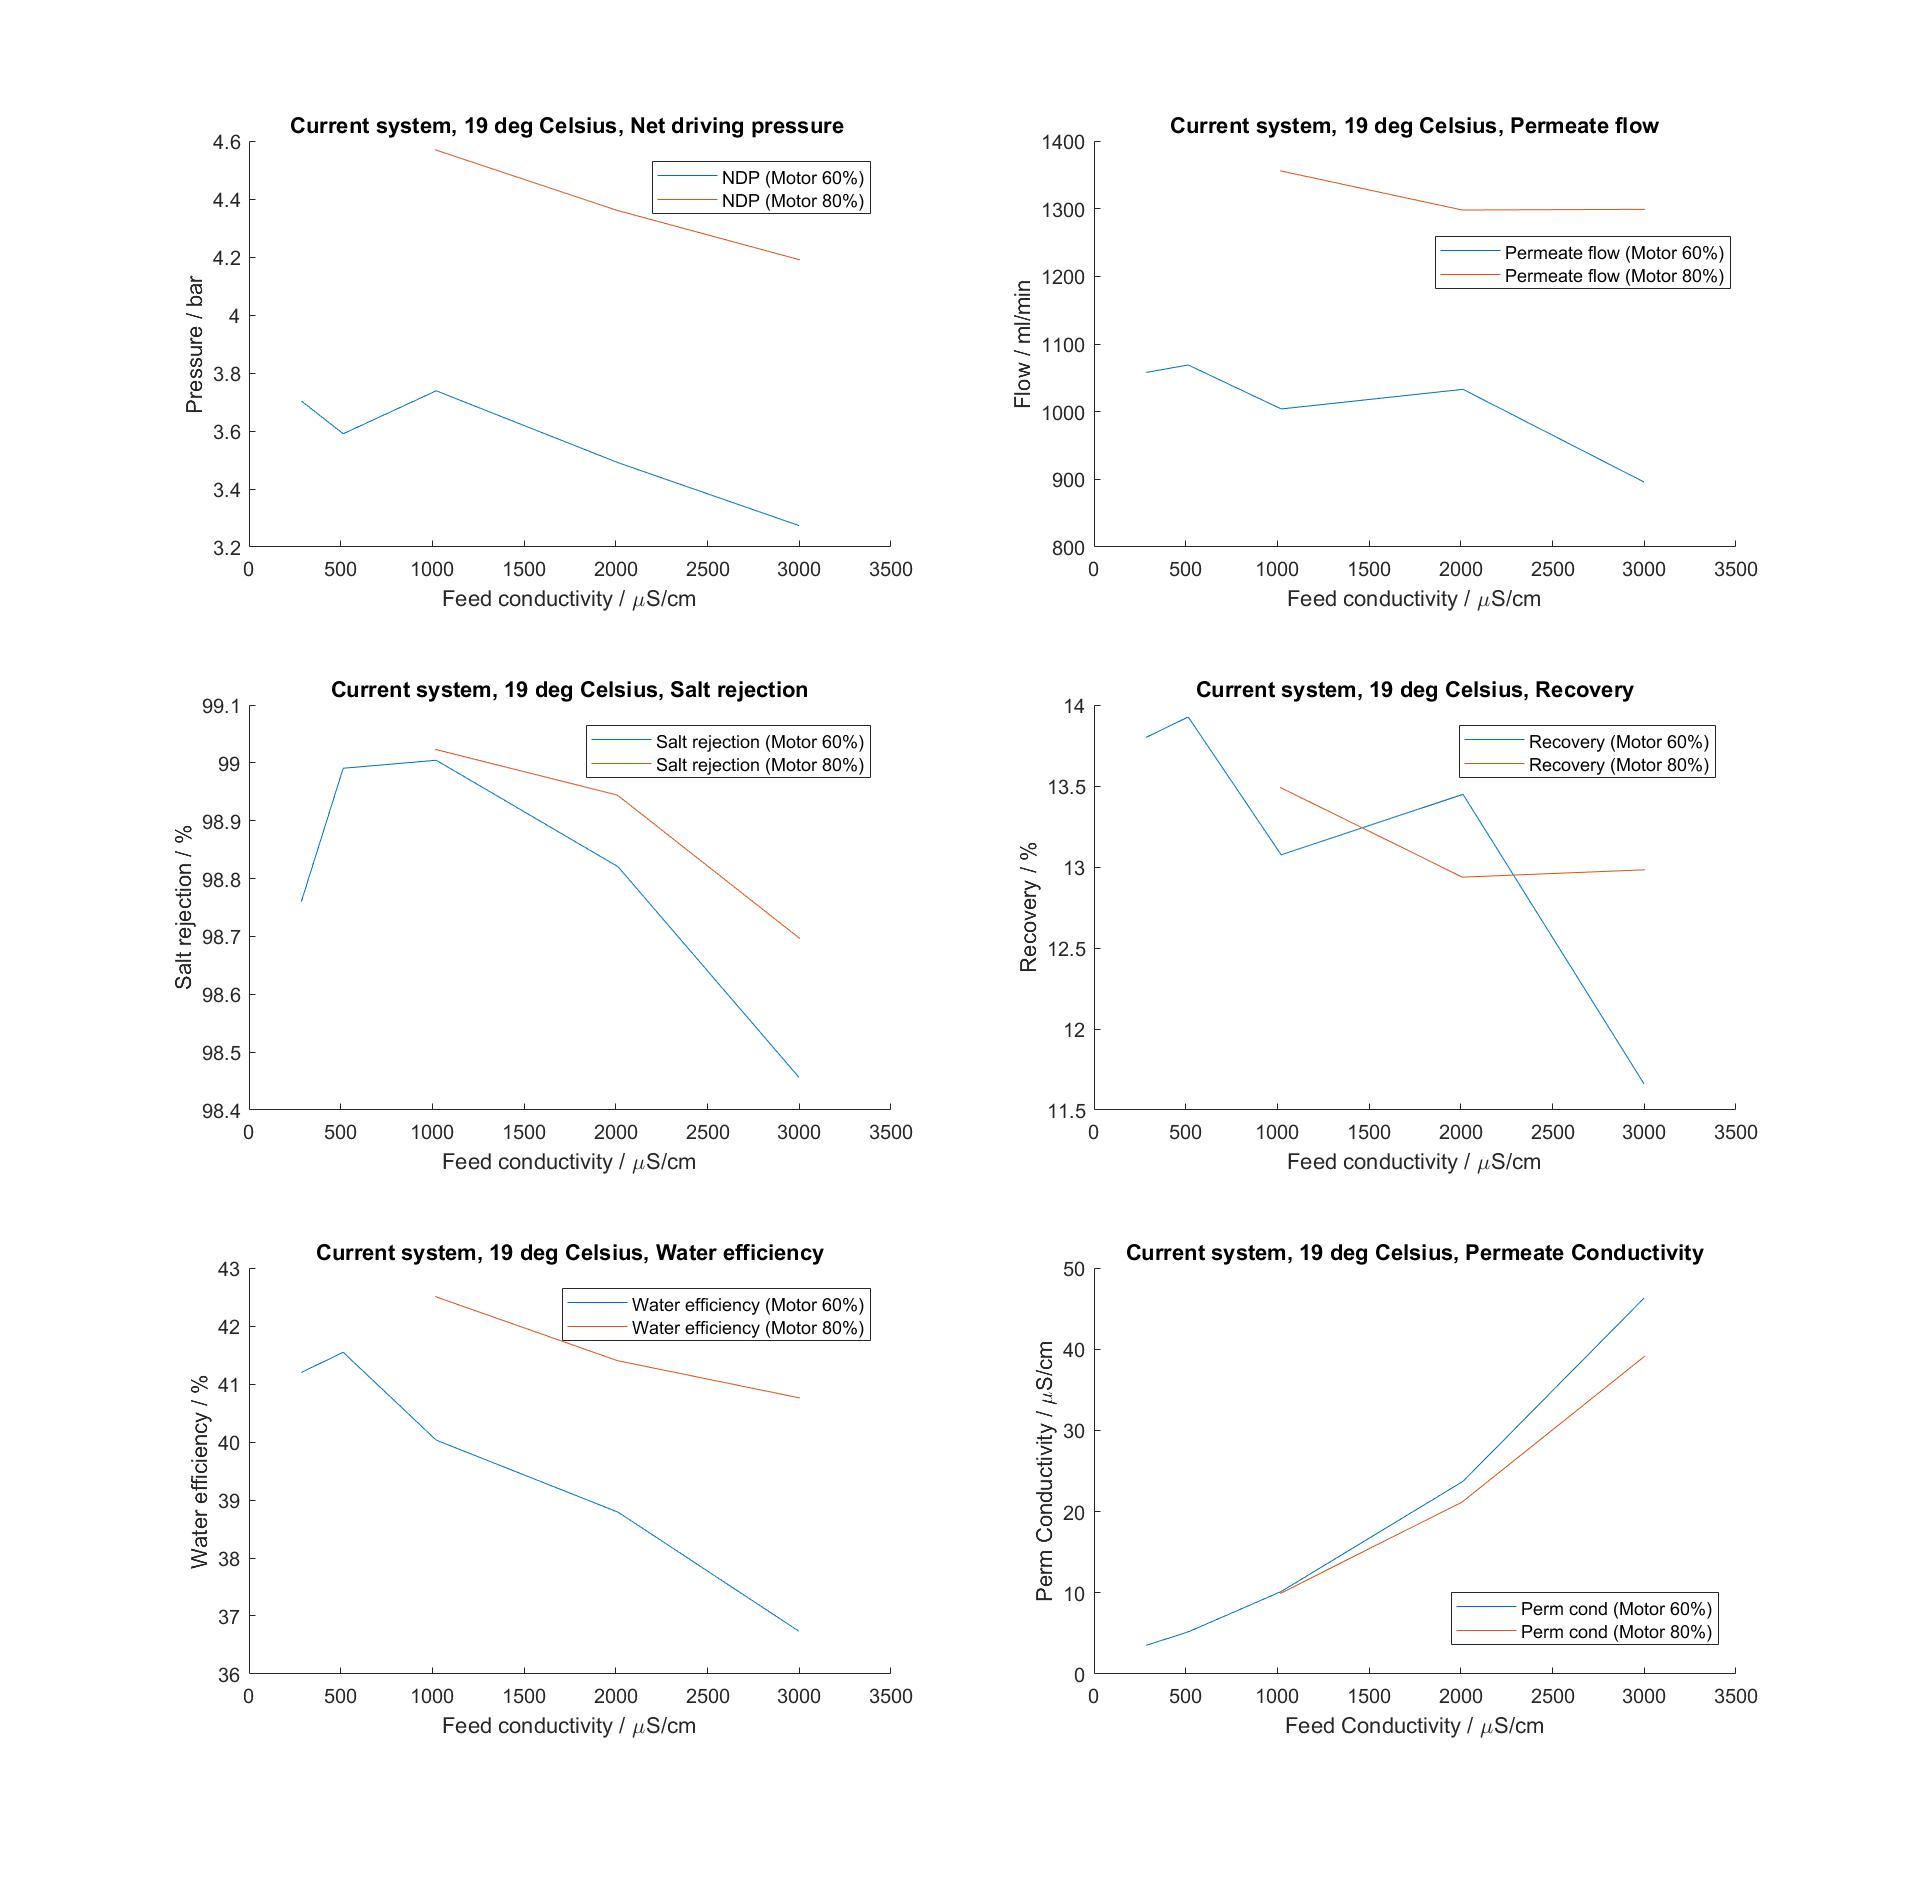
\includegraphics[width=1.1\textwidth]{Key20}
    \caption{Caption missing}
    \label{fig:PressConn}
\end{figure}

\newpage

\subsection{Current system, Test sequence 2}

The second test was carried out by setting the heater bath to 30 degrees celsius and and adjusting the conductivity and pump speed according to the test plan. Since the water was much warmer than the air in the room, the heating caused by the pump was not as prominent and allowed all steady states to be examined in one continous test.

\begin{figure}[H]
    \centering
    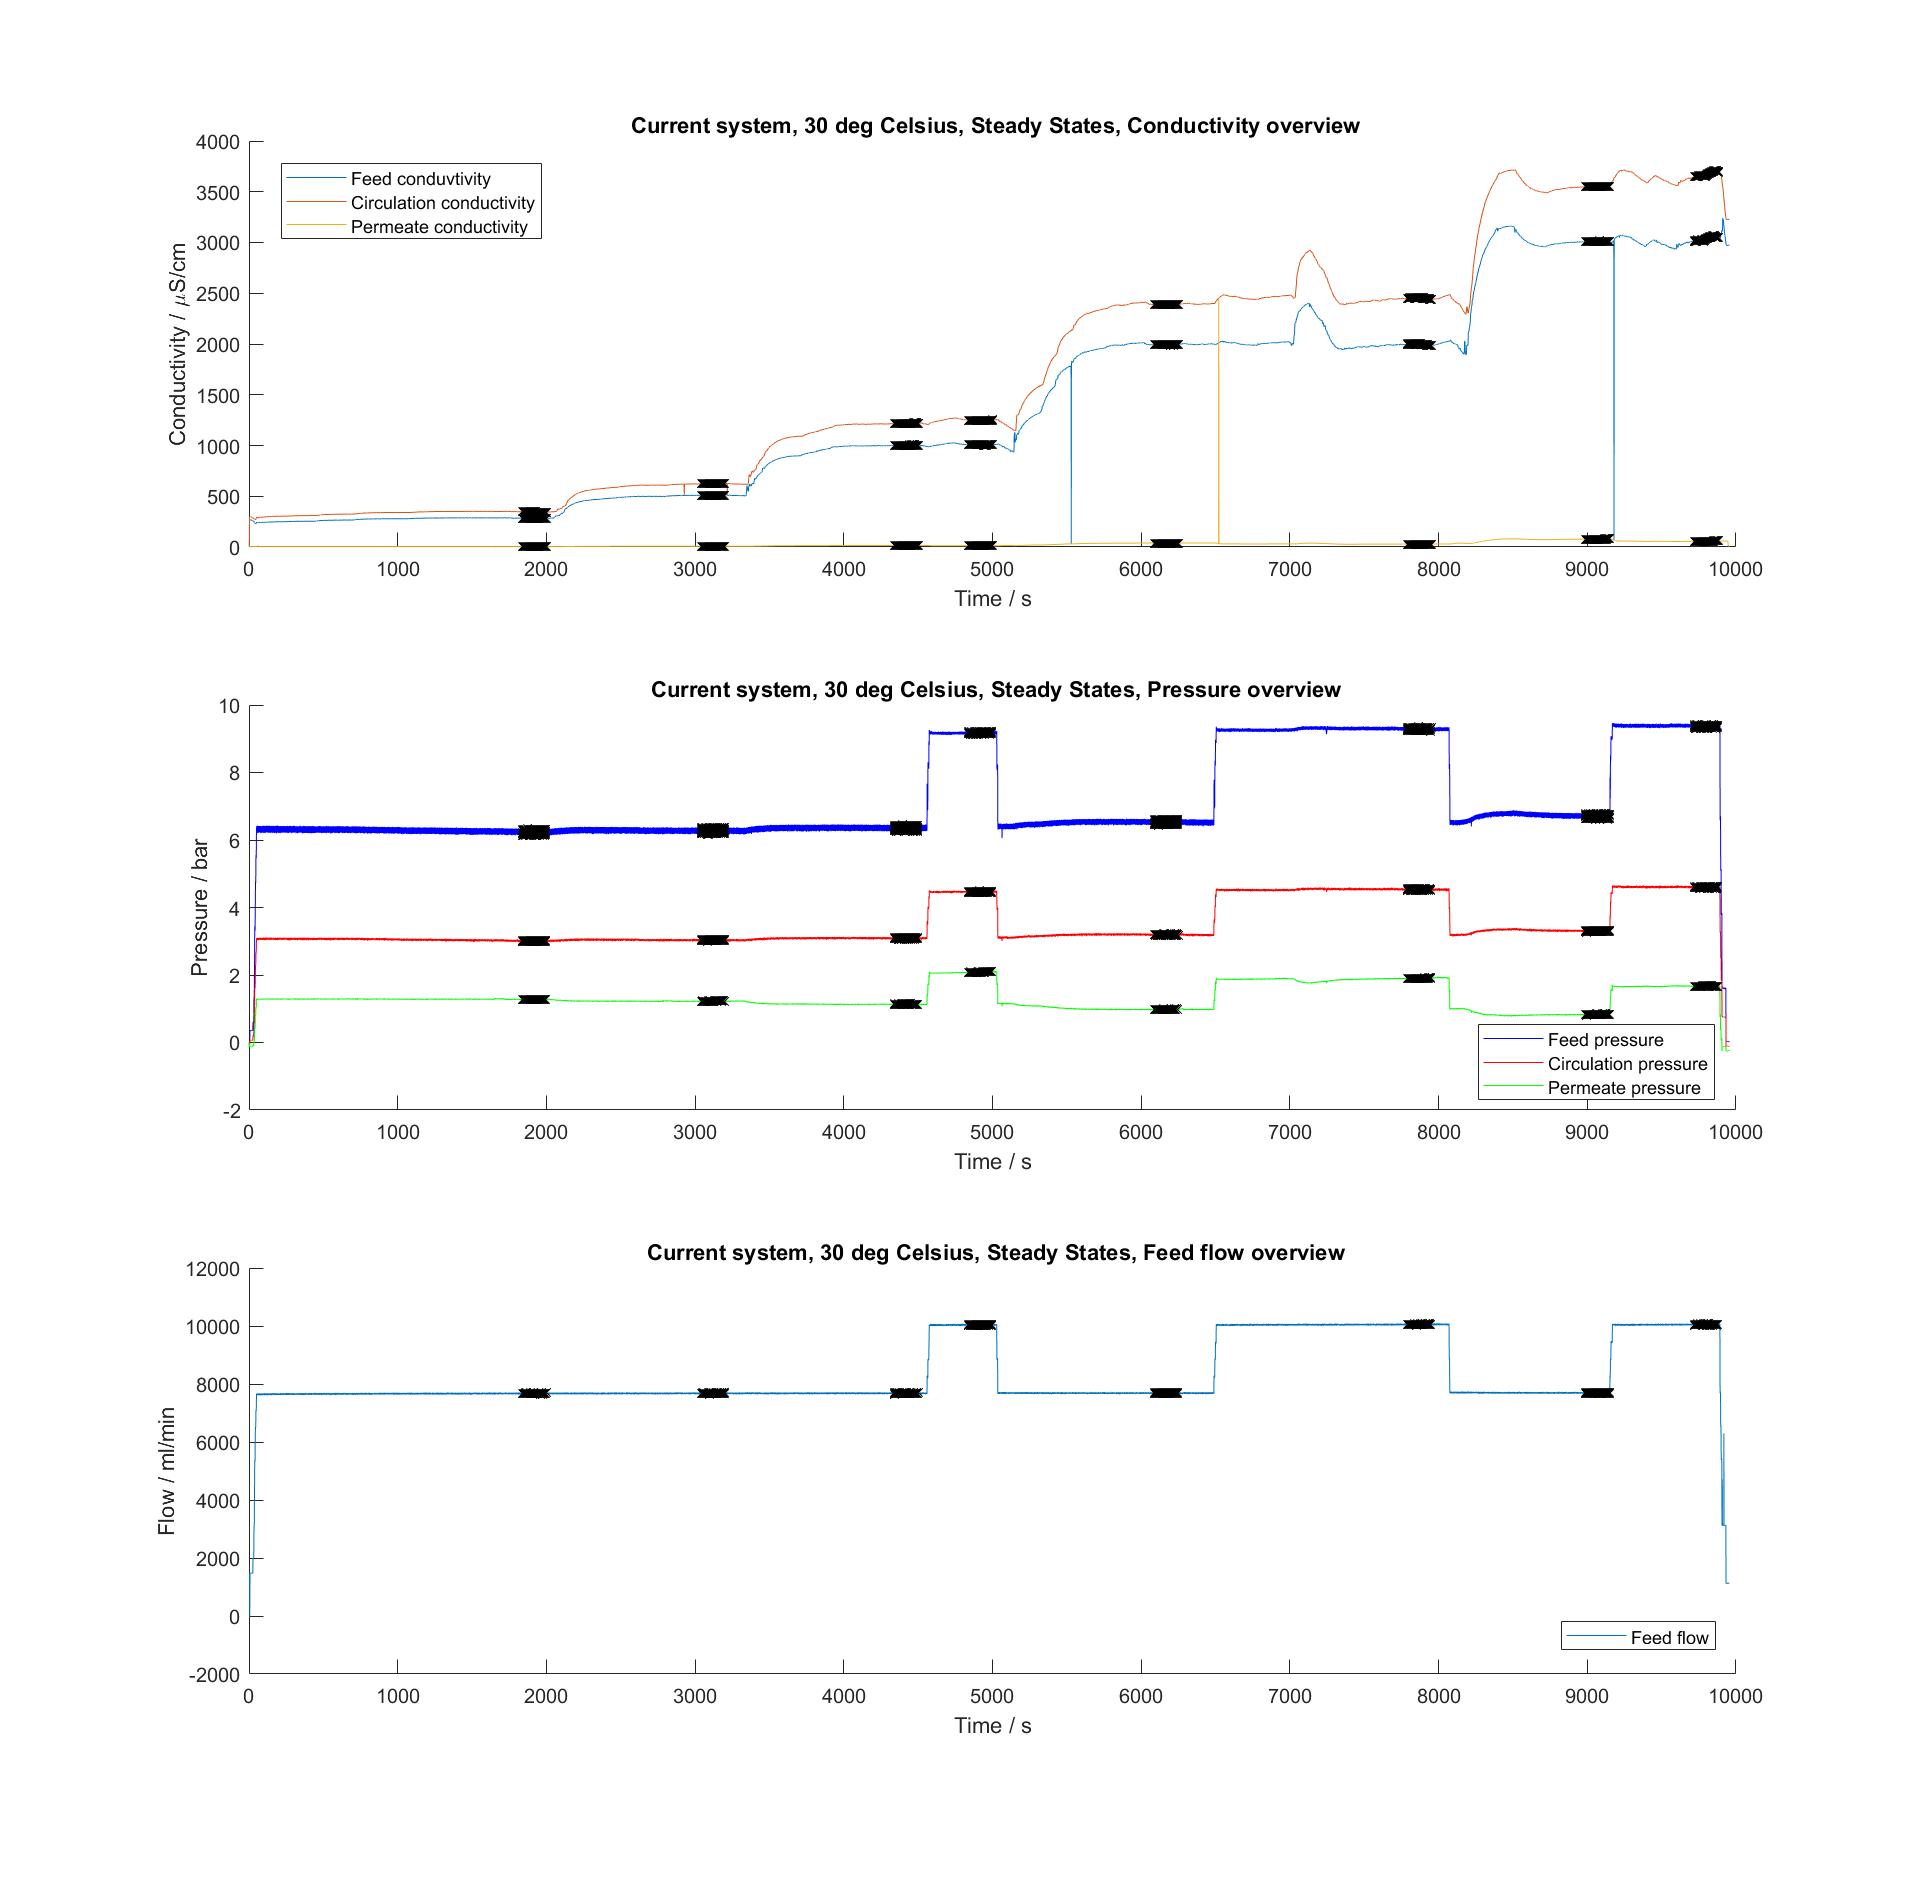
\includegraphics[width=1.1\textwidth]{overview30}
    \caption{Test 2, Current system, 30 degrees celsius. Steady states 1.1, 1.2, 1.3, 1.4 1.5, 1.6, 1.7 and 1.8}
    \label{fig:PressConn}
\end{figure}

\newpage


The data from the test was post processed in Matlab in exactly the same way as the previous test.

\begin{figure}[H]
    \centering
    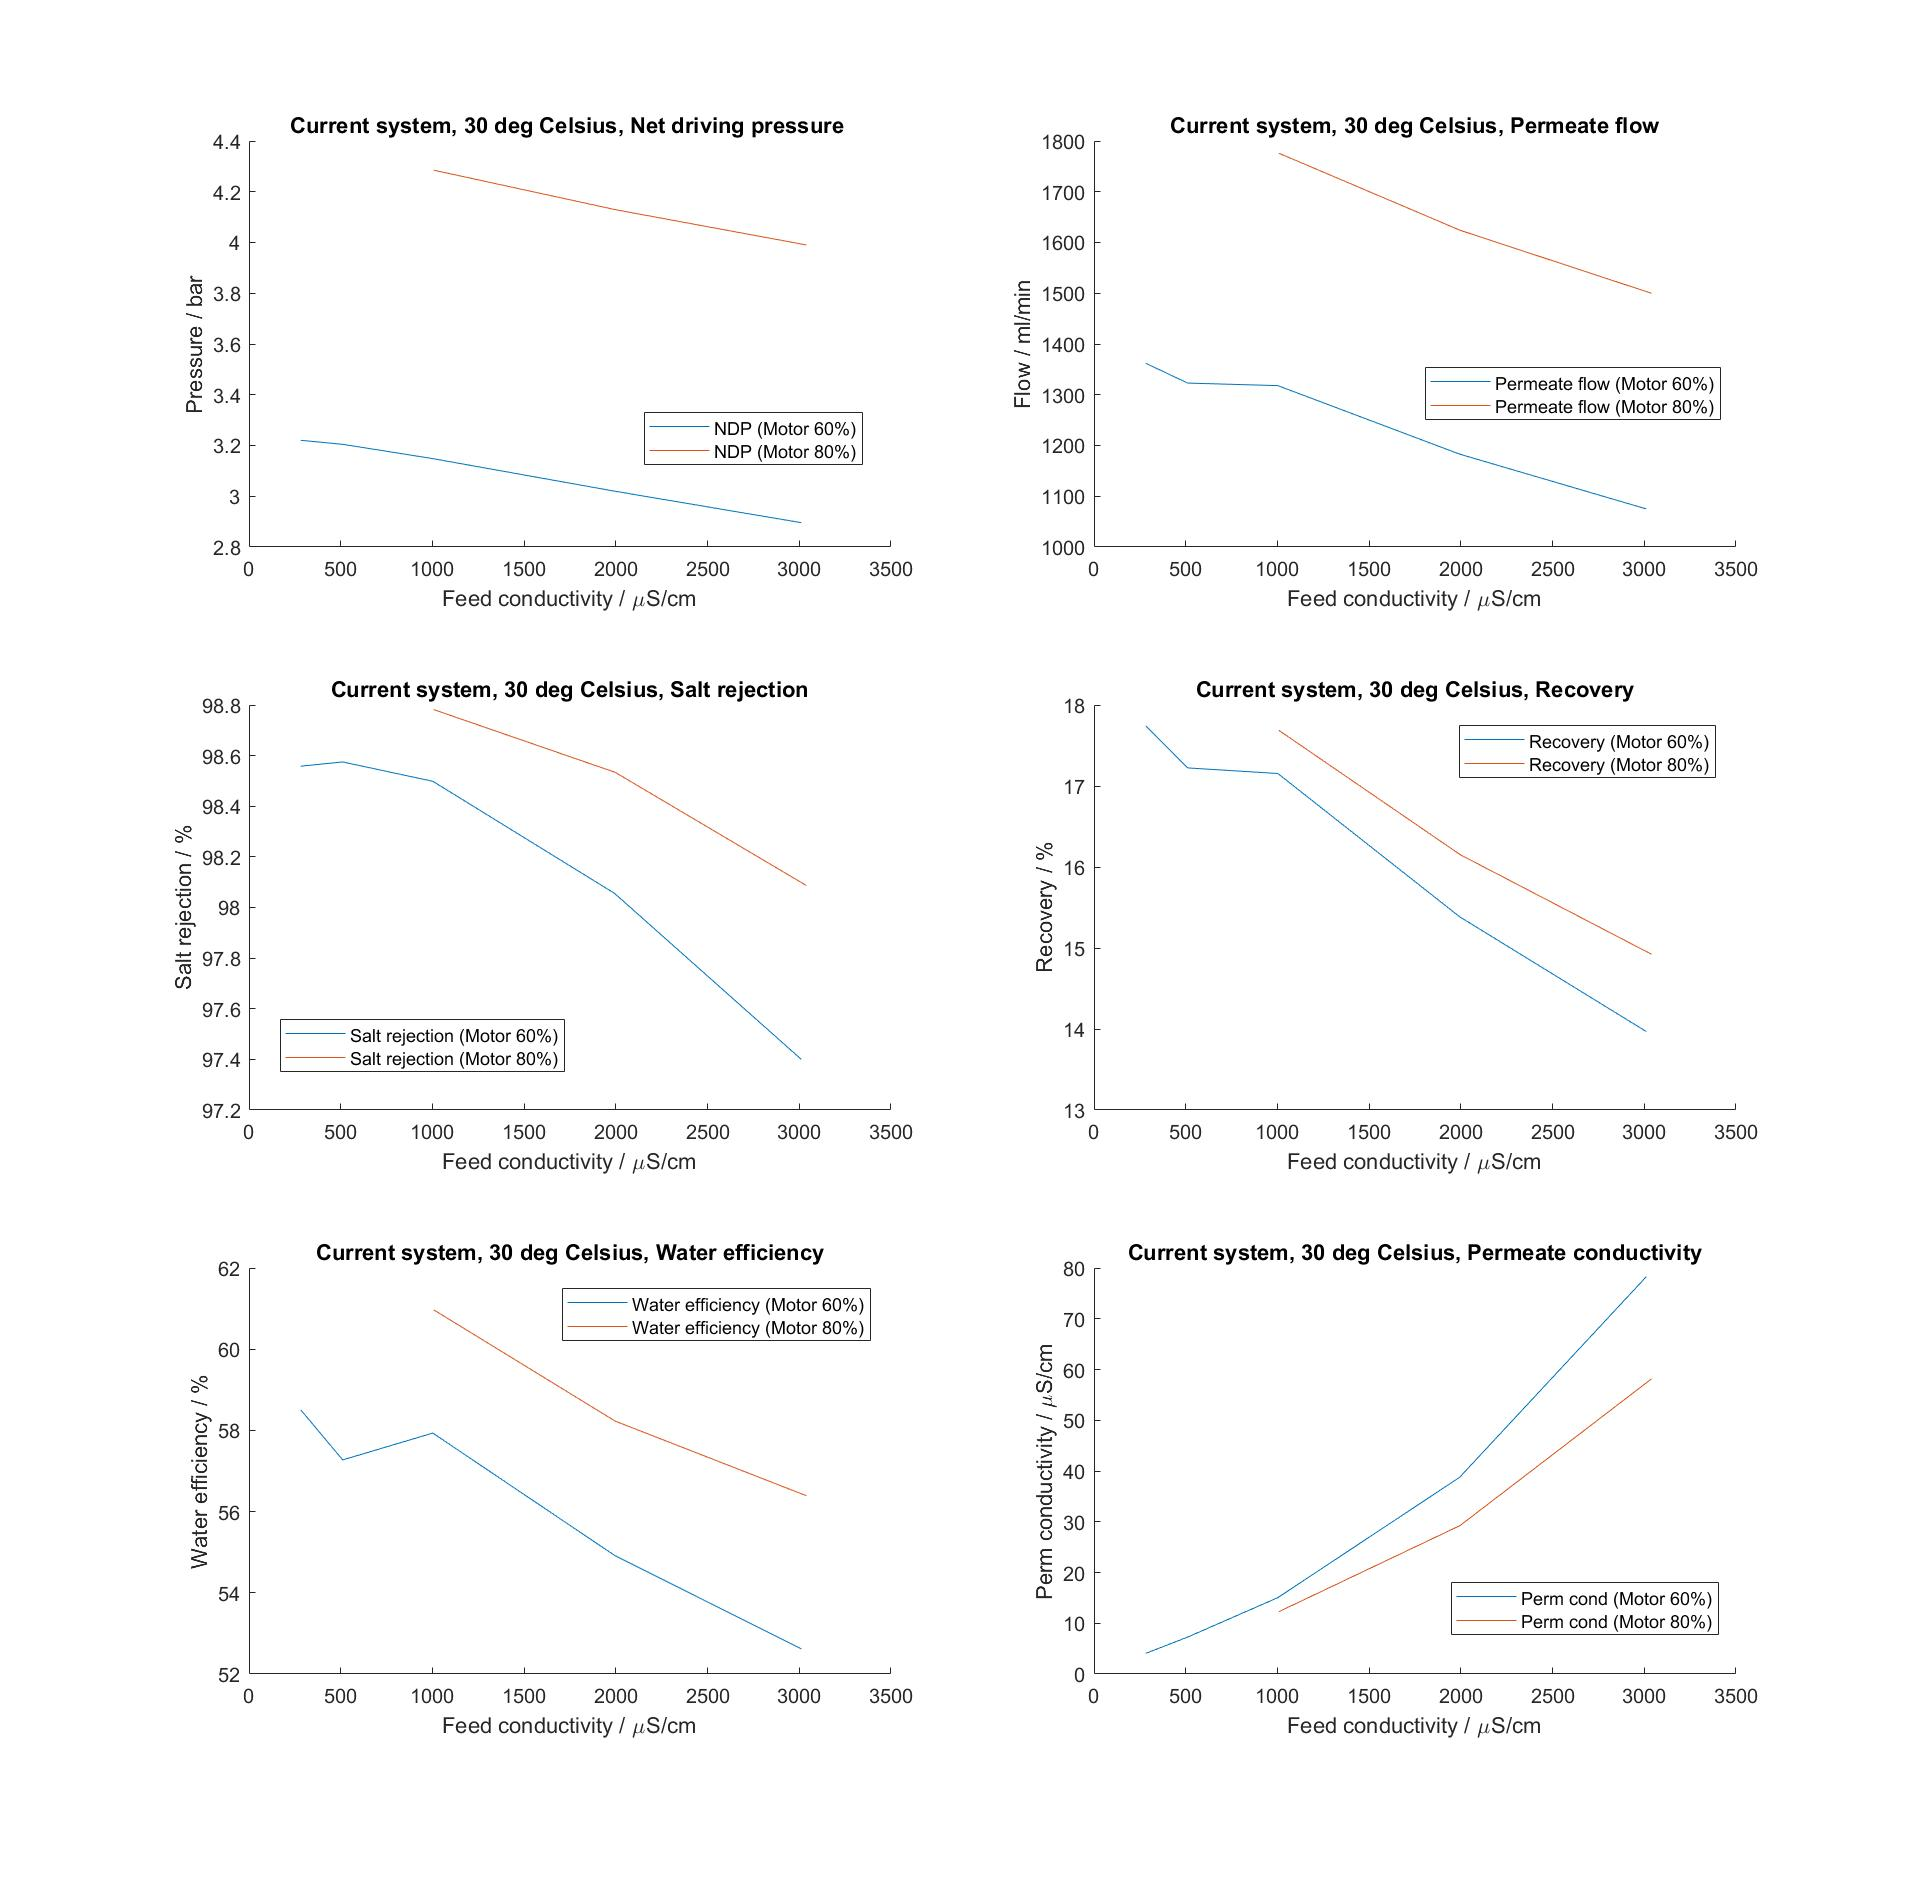
\includegraphics[width=1.1\textwidth]{Key30}
    \caption{Caption missing}
    \label{fig:PressConn}
\end{figure}

\newpage

\subsection{Current system, Test sequence 3}

Finally the heating bath was set to 40 C and the test sequence was performed just like test sequence 2. 

\begin{figure}[H]
    \centering
    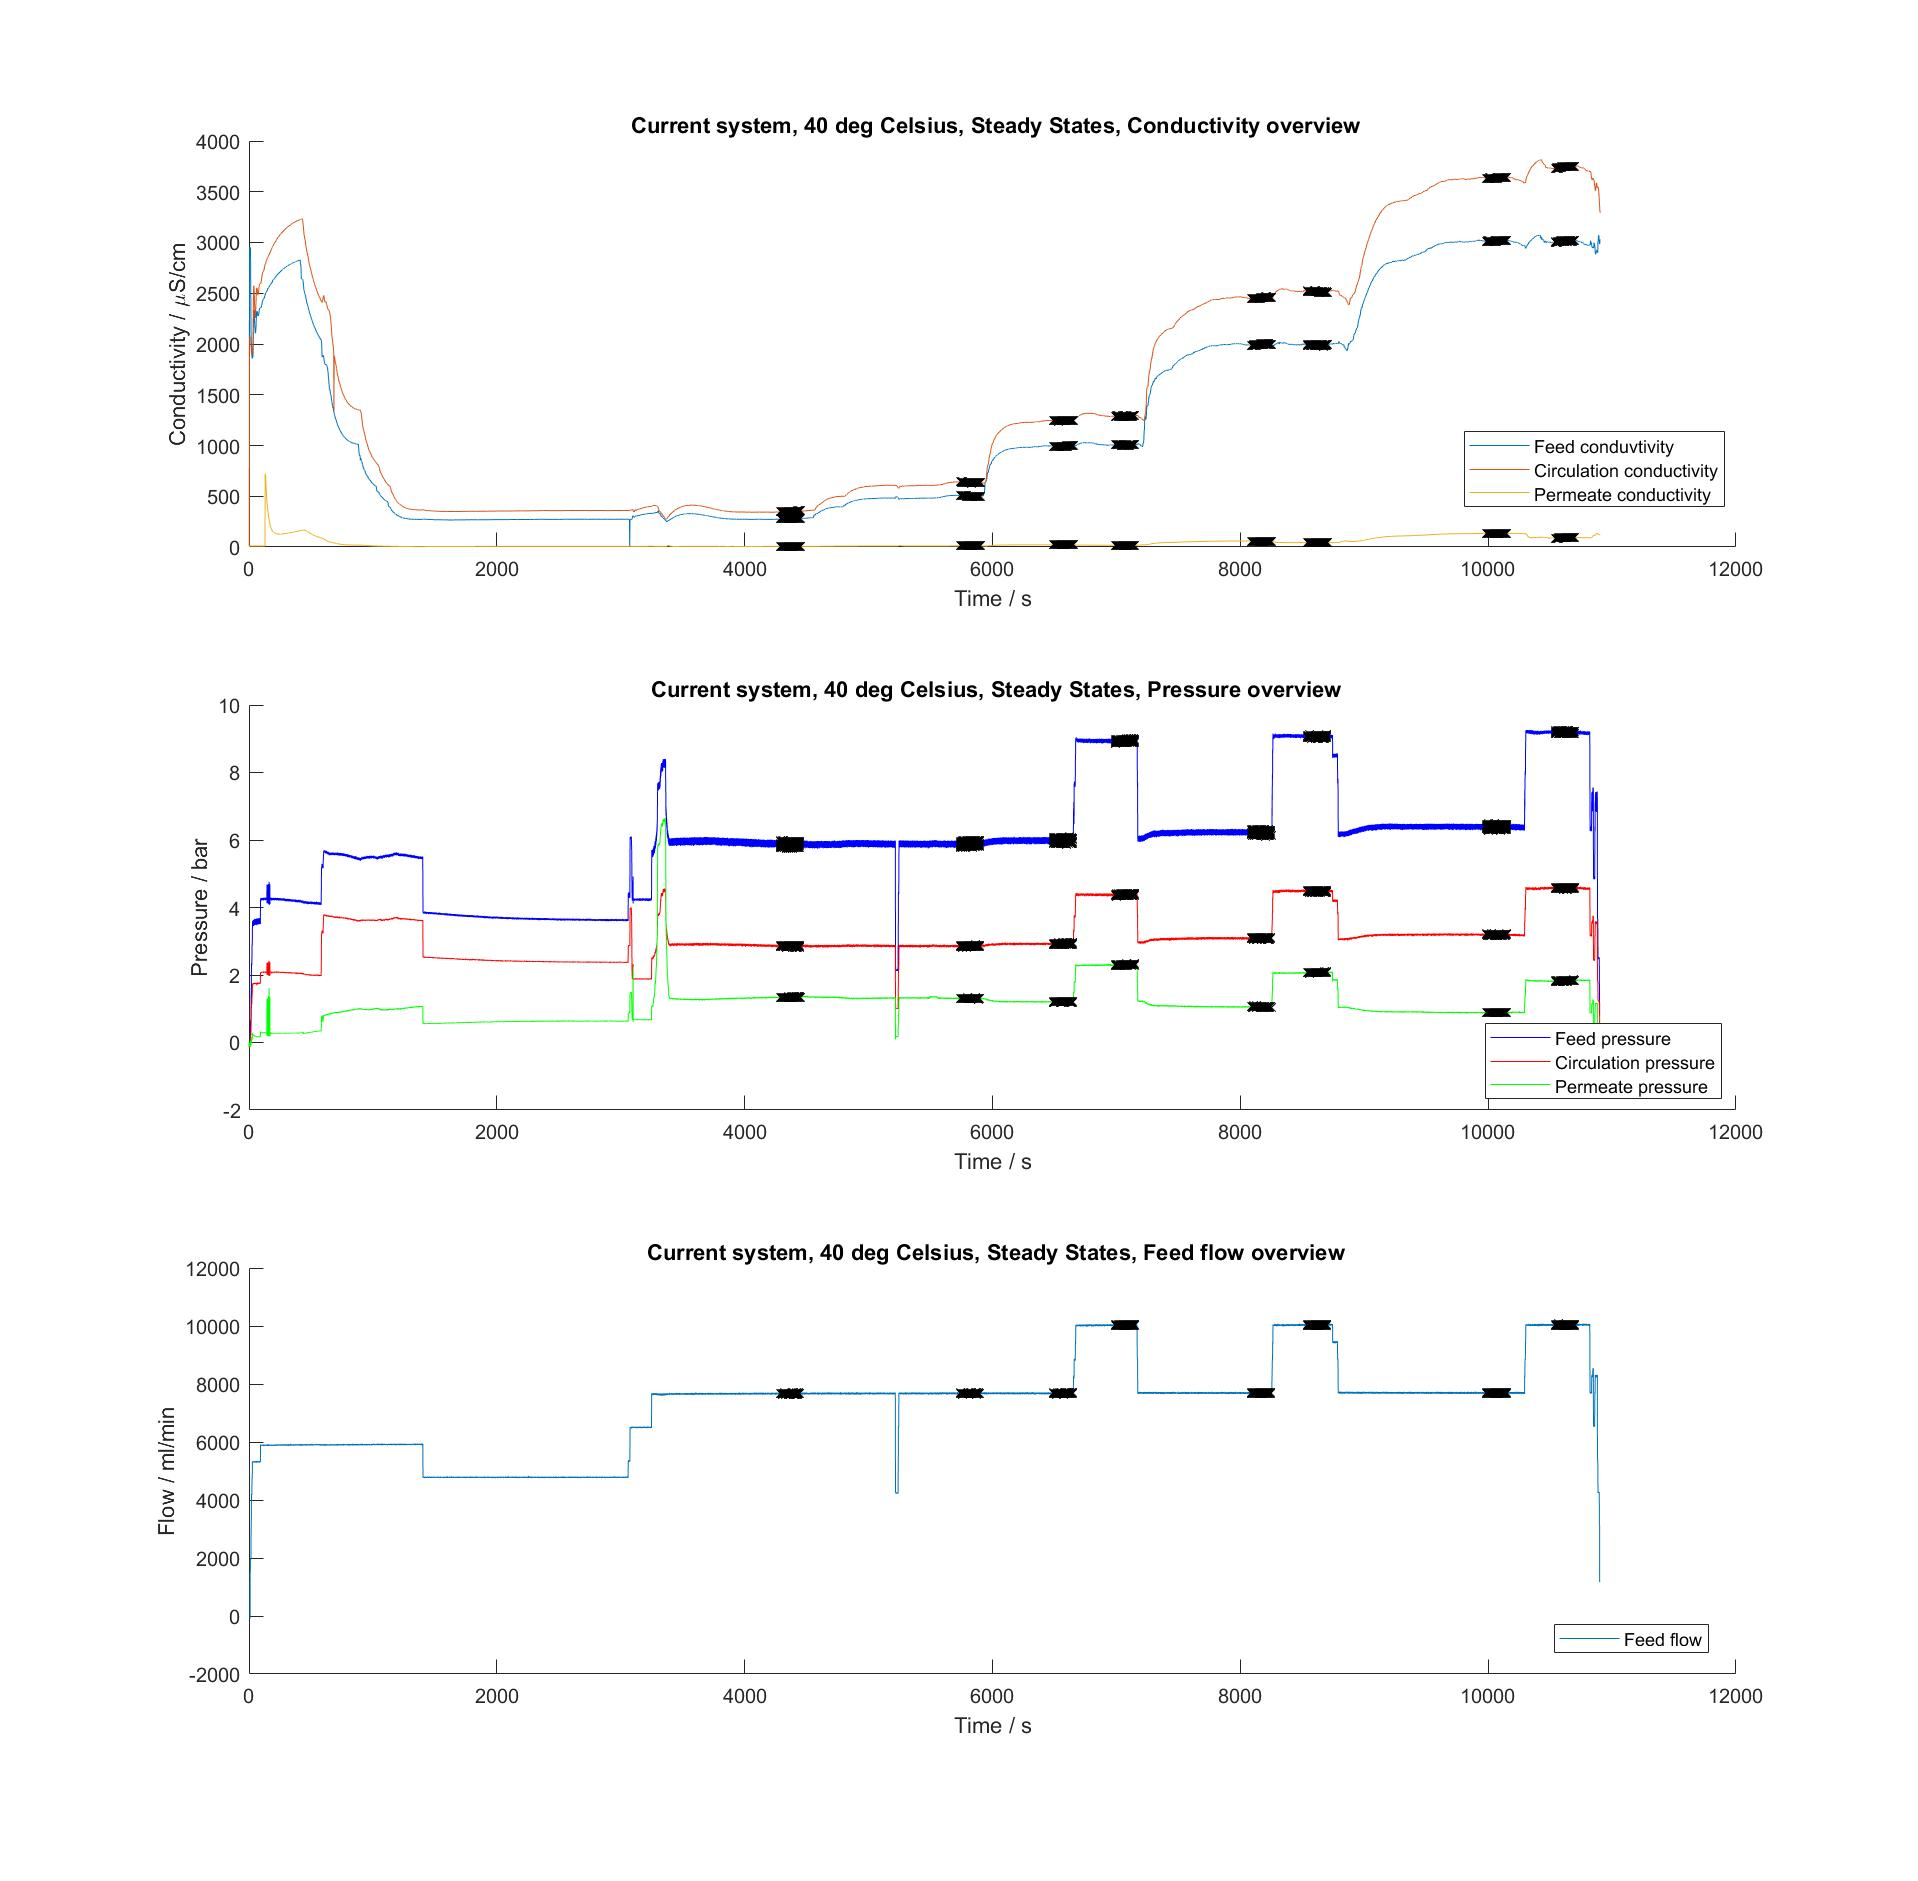
\includegraphics[width=1.1\textwidth]{overview40}
    \caption{Caption missing}
    \label{fig:PressConn}
\end{figure}

\newpage

Post processing in matlab generated the following data from the steady states.

\begin{figure}[H]
    \centering
    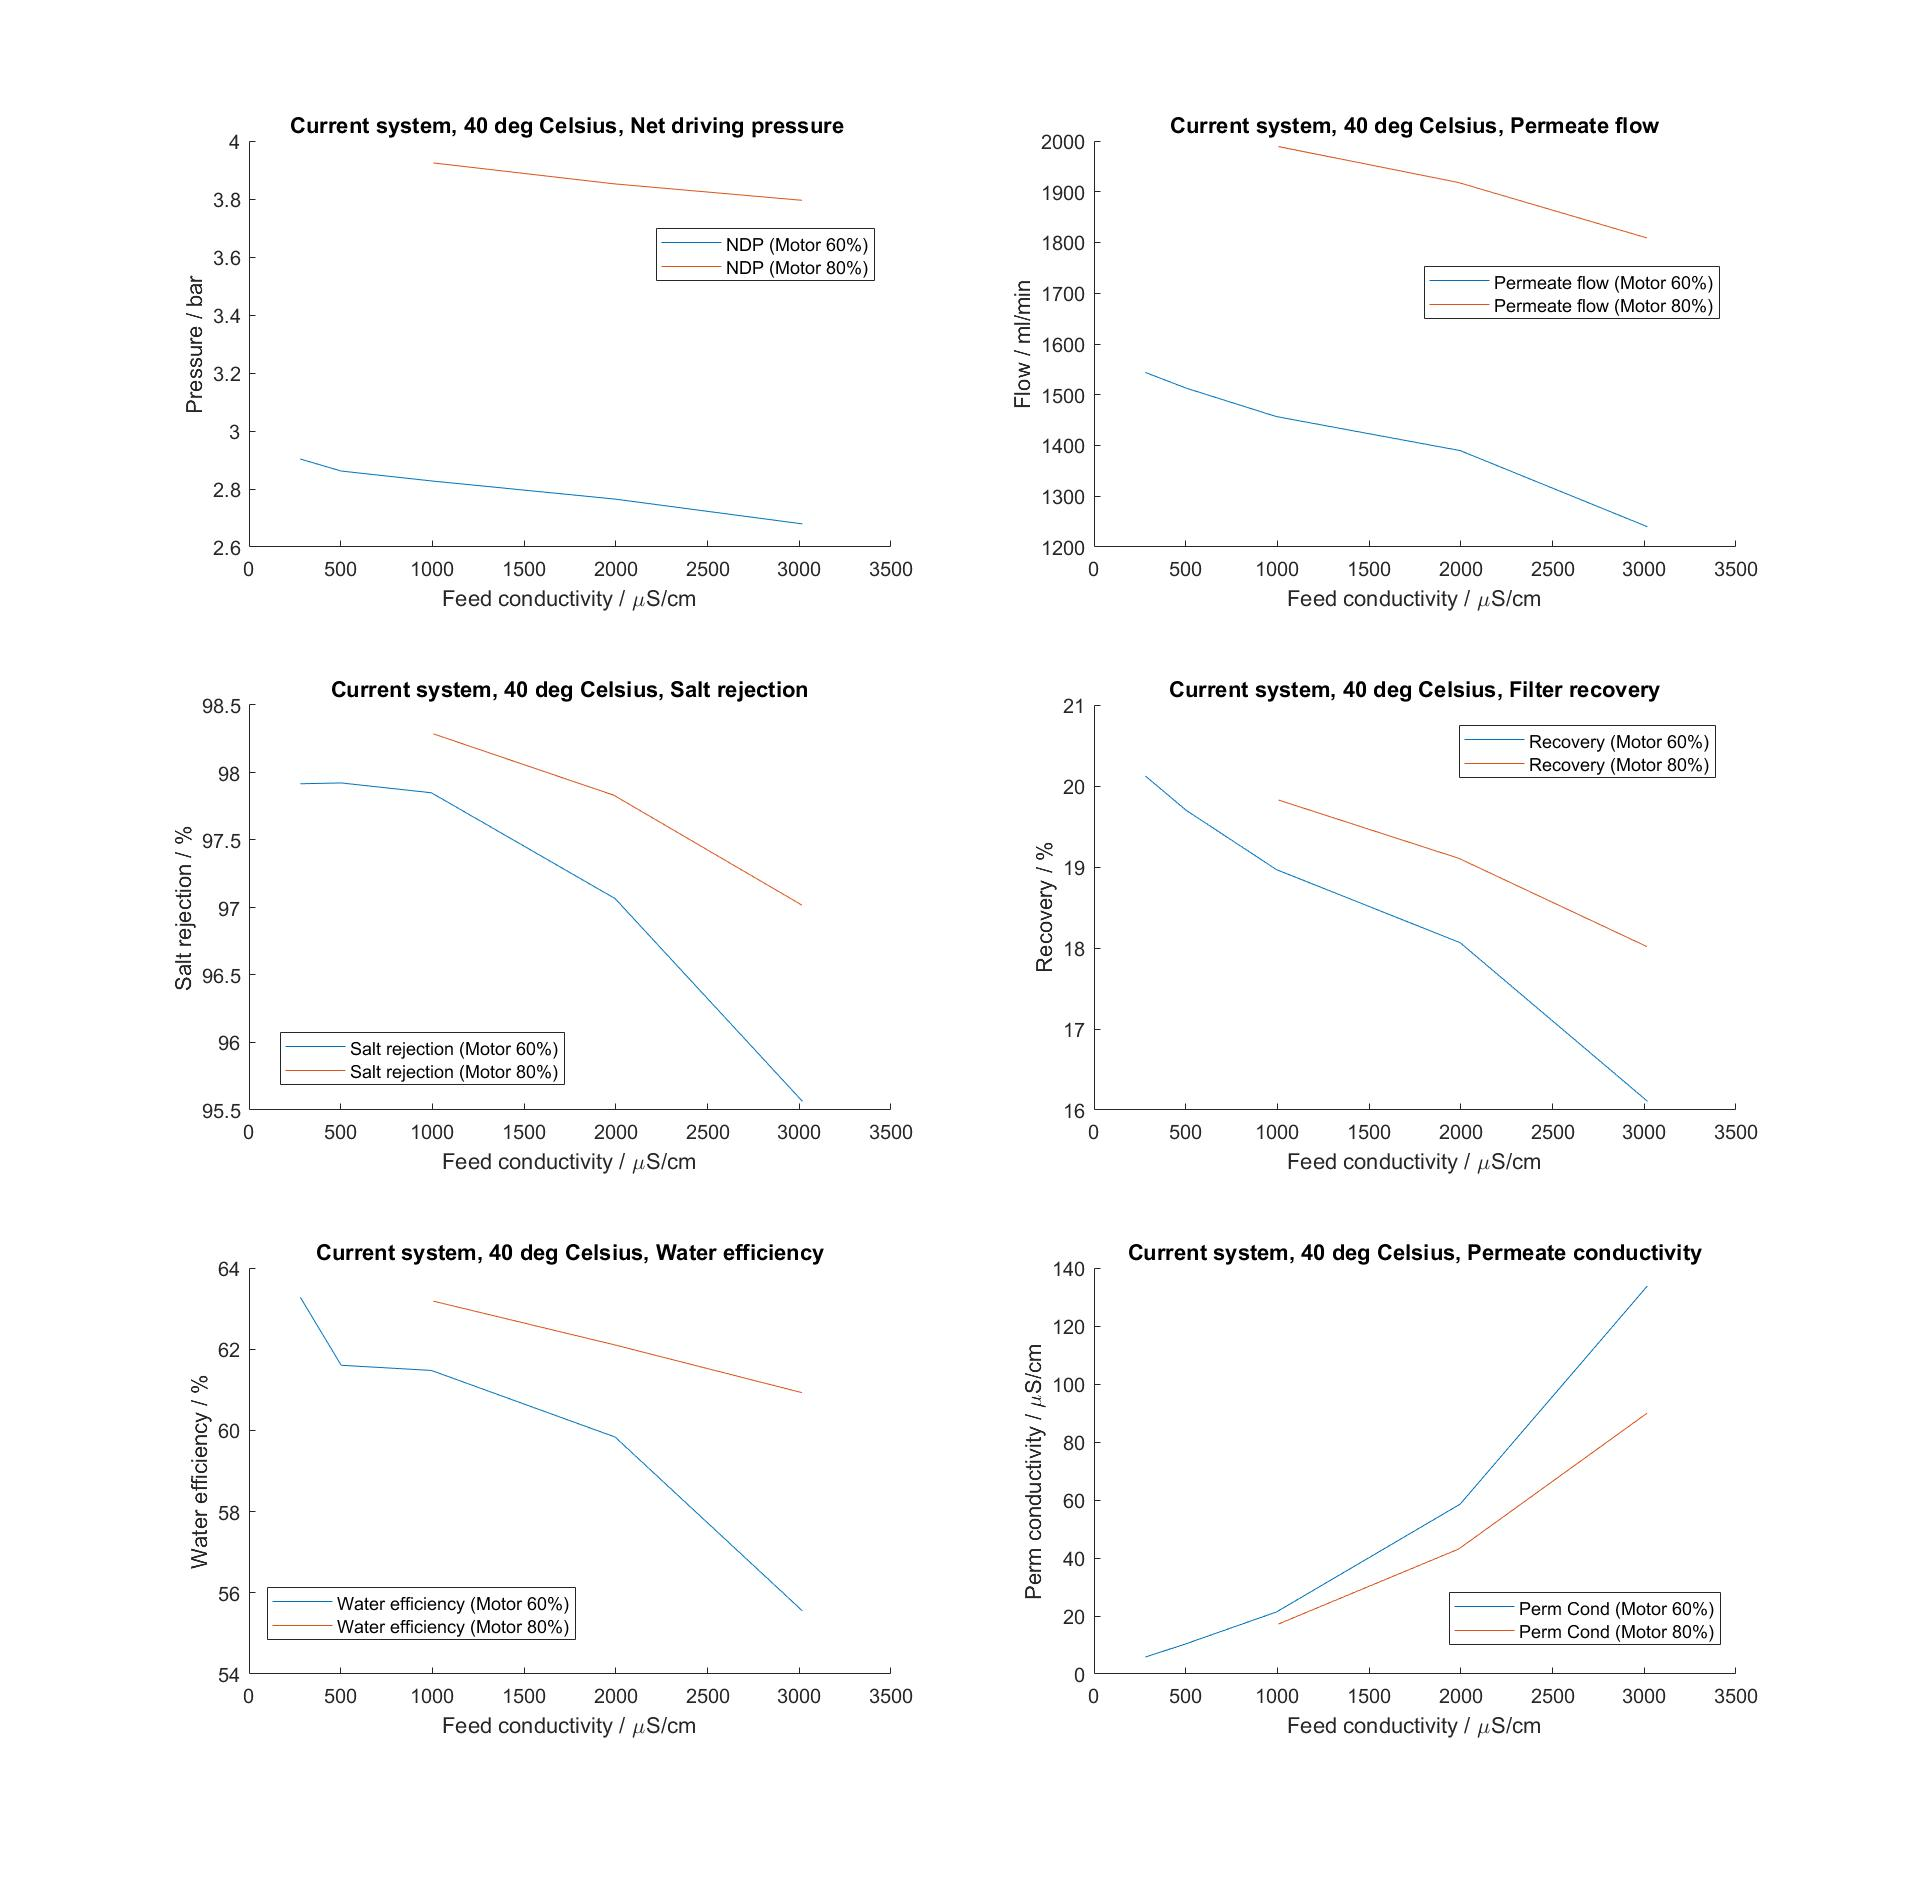
\includegraphics[width=1.1\textwidth]{Key40}
    \caption{Caption missing}
    \label{fig:PressConn}
\end{figure}

\newpage

In order to understand how the system current performed in different working conditions all plots from the post processing in Matlab was put togheter. 

\subsection{Net driving pressure}

Net driving pressure was decreased when the temperature was increased. Higher feed conductivity resulted in a decreased net driving pressure. As expected, running the feed pump at a higher RPM also increased the net driving pressure.

\begin{figure}[H]
    \centering
    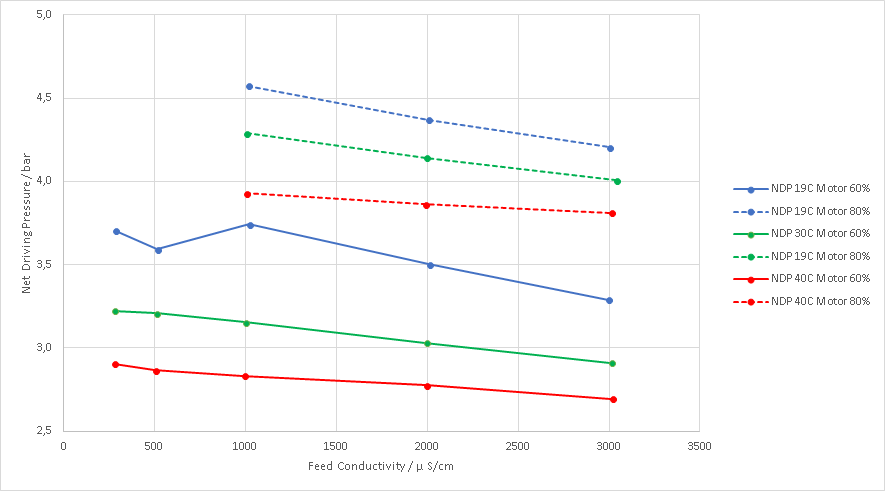
\includegraphics[width=0.8\textwidth]{NDP}
    \caption{Net driving pressure}
    \label{fig:NDP}
\end{figure}

\subsection{Permeate flow}

According to theory, Net driving pressure has a direct effect on permeate flow. When the feed pump was increased more water was pushed through the membrane. Increased water temperatures caused a much higher permeate flow. For instance, the permeate flow increased by around 50\% when the temperature was increased from 19 C to 40 C and the pump was running at 60\%. Due to the increased osmotic pressure, permeate flow decreased when the feed conductivity increased

\begin{figure}[H]
    \centering
    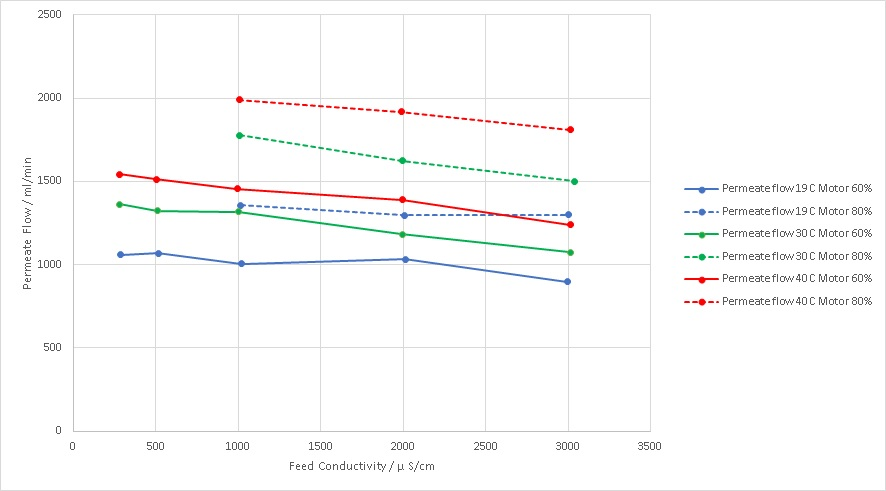
\includegraphics[width=0.8\textwidth]{permFlowCurrent}
    \caption{Caption missing}
    \label{fig:PressConn}
\end{figure}

\subsection{Recovery}

Warmer water enabled more feed water to pass through the membrane and therefore the recovery was increased. Increased conductivity reduced recovery due to the increased osmotic pressure.

\begin{figure}[H]
    \centering
    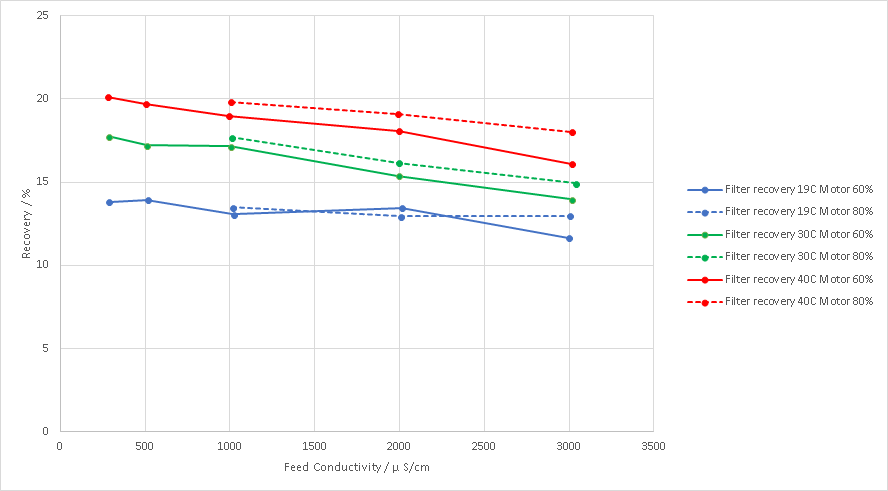
\includegraphics[width=0.8\textwidth]{Recovery}
    \caption{Caption missing}
    \label{fig:PressConn}
\end{figure}

\subsection{Salt rejection}

By looking at plot 5.13 the deterimental effects of both increased temperature and feed conductivity can be seen. The negative effect of increased feed conductivity was much more prominent at 40 C than 30C which means that the performance of the membrane decreased exponentially with higher temperature. Increased feed pump pressure resultet in better salt rejection and the positive effect of increased pump pressure was larger when the system was hot. Temperature was the parameter that decreased salt rejetion the most and by comparing how the system performed when the pump and feed conductivity was set to 60\% and 3000uS/cm at 19C and 40C it can be seen that the salt rejection decreased from 98.5\% to 95.5 \%. From the experiment it can also be concluded that the system perform much better at low temperature and feed conductivity that at high temperature and feed conductivity. 

\begin{figure}[H]
    \centering
    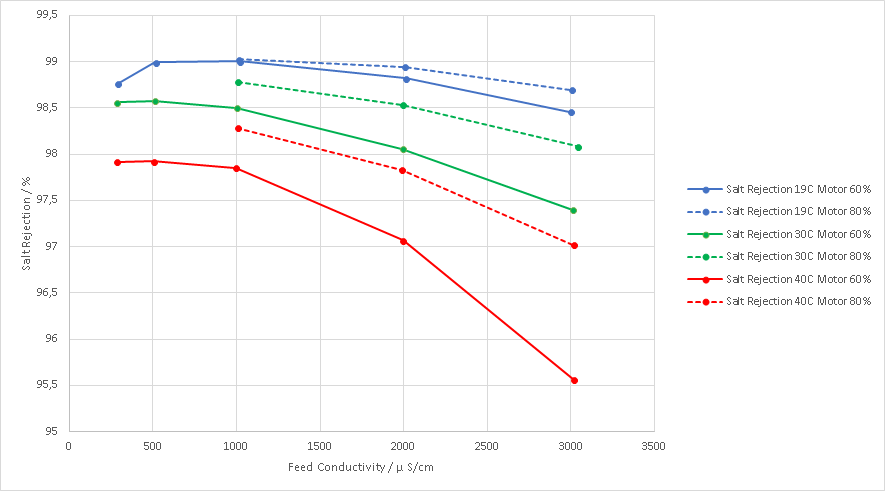
\includegraphics[width=0.8\textwidth]{SaltRejection}
    \caption{Saltrejection}
    \label{fig:SalrRejectionResult}
\end{figure}
 
\subsection{Permeate conductivity}

Permeate conductivity was directly proportional to salt rejection at a certain termperature and feed conductivity. The black line in plot 5.14 show the critical permeate conductivity that the system should be able to maintain and from the plot it is possible to se how high the conductivity can be in the recirculation loop without exceeding this limit. The operational area for the different temperature and pump pressure can be seen in plot TBD below.

\begin{figure}[H]
    \centering
    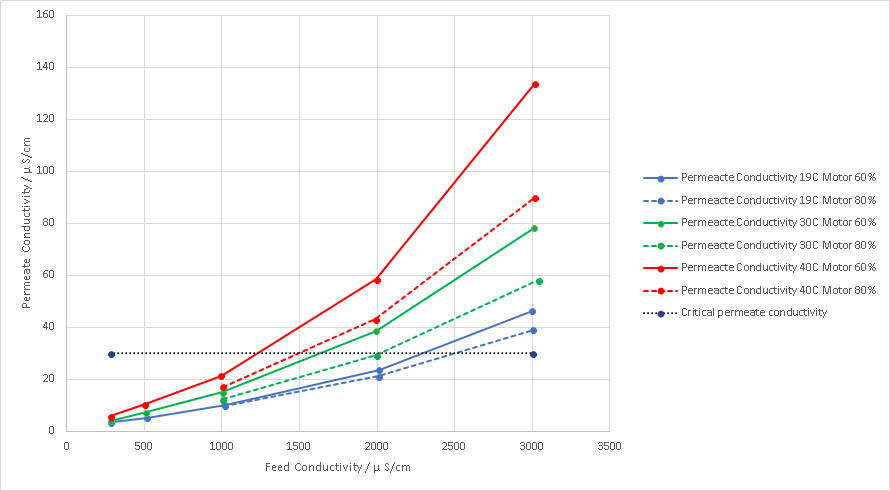
\includegraphics[width=0.8\textwidth]{PermCond}
    \caption{Conductivity}
    \label{fig:PressConn}
\end{figure}

!!INSERT TABLE!!

\subsection{Water efficiency}

Water efficiency increased when the temperature increased due to more permeate water being generated by the same feed pressure.

\begin{figure}[H]
    \centering
    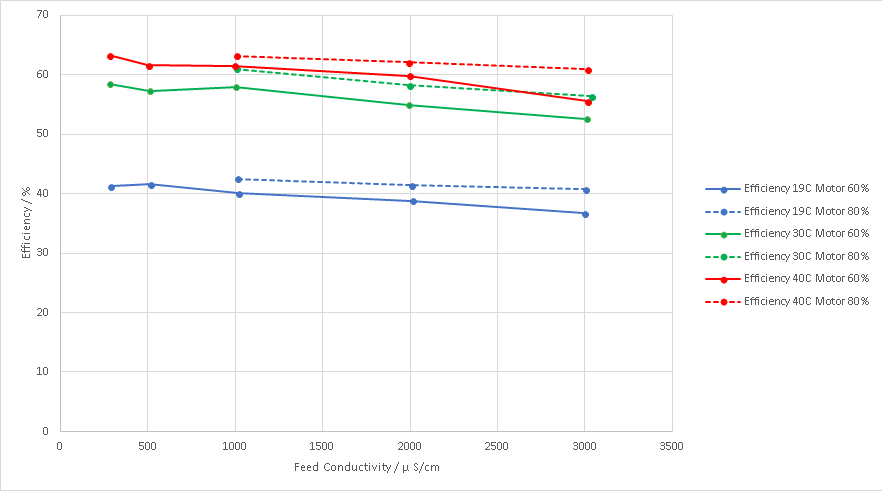
\includegraphics[width=0.8\textwidth]{Efficiency}
    \caption{Efficiency}
    \label{fig:PressConn}
\end{figure}

\newpage

\subsection{System 2}

The circulation pump and a flow meter was added to the system and the flow path was modified according to figure XXXX. The rig was also reprogrammed to be able to measure all flows in the flow path in real time. This could be done because now both the feed flow, circulation flow and permeate flow could be measured and from this data, the inlet and drain flow could be calculated. 


\newpage
\subsubsection{Increased circulation}

The Initial idea for optimizing the membrane was to use the circulation pump to create a turbulent flow close to the membrane surface. Therefore, a test was set up to test this idea.
During the test, the feed pump and drain valve was set to a fixed value and the circulation pump was increased from 5\% to 35\%. Figure \ref{fig:RecIncrease} show the permeate conductivity, circulation flow and feed pressure and 7 steady state points from the test.

The circulation flow was increased from 1500 ml/min to 5000 ml/min and the increased circulation flow caused the pressure to increase from 5.5 to 7 bar. The permeate conductivity remained unchanged. 
\begin{figure}[H]
    \centering
    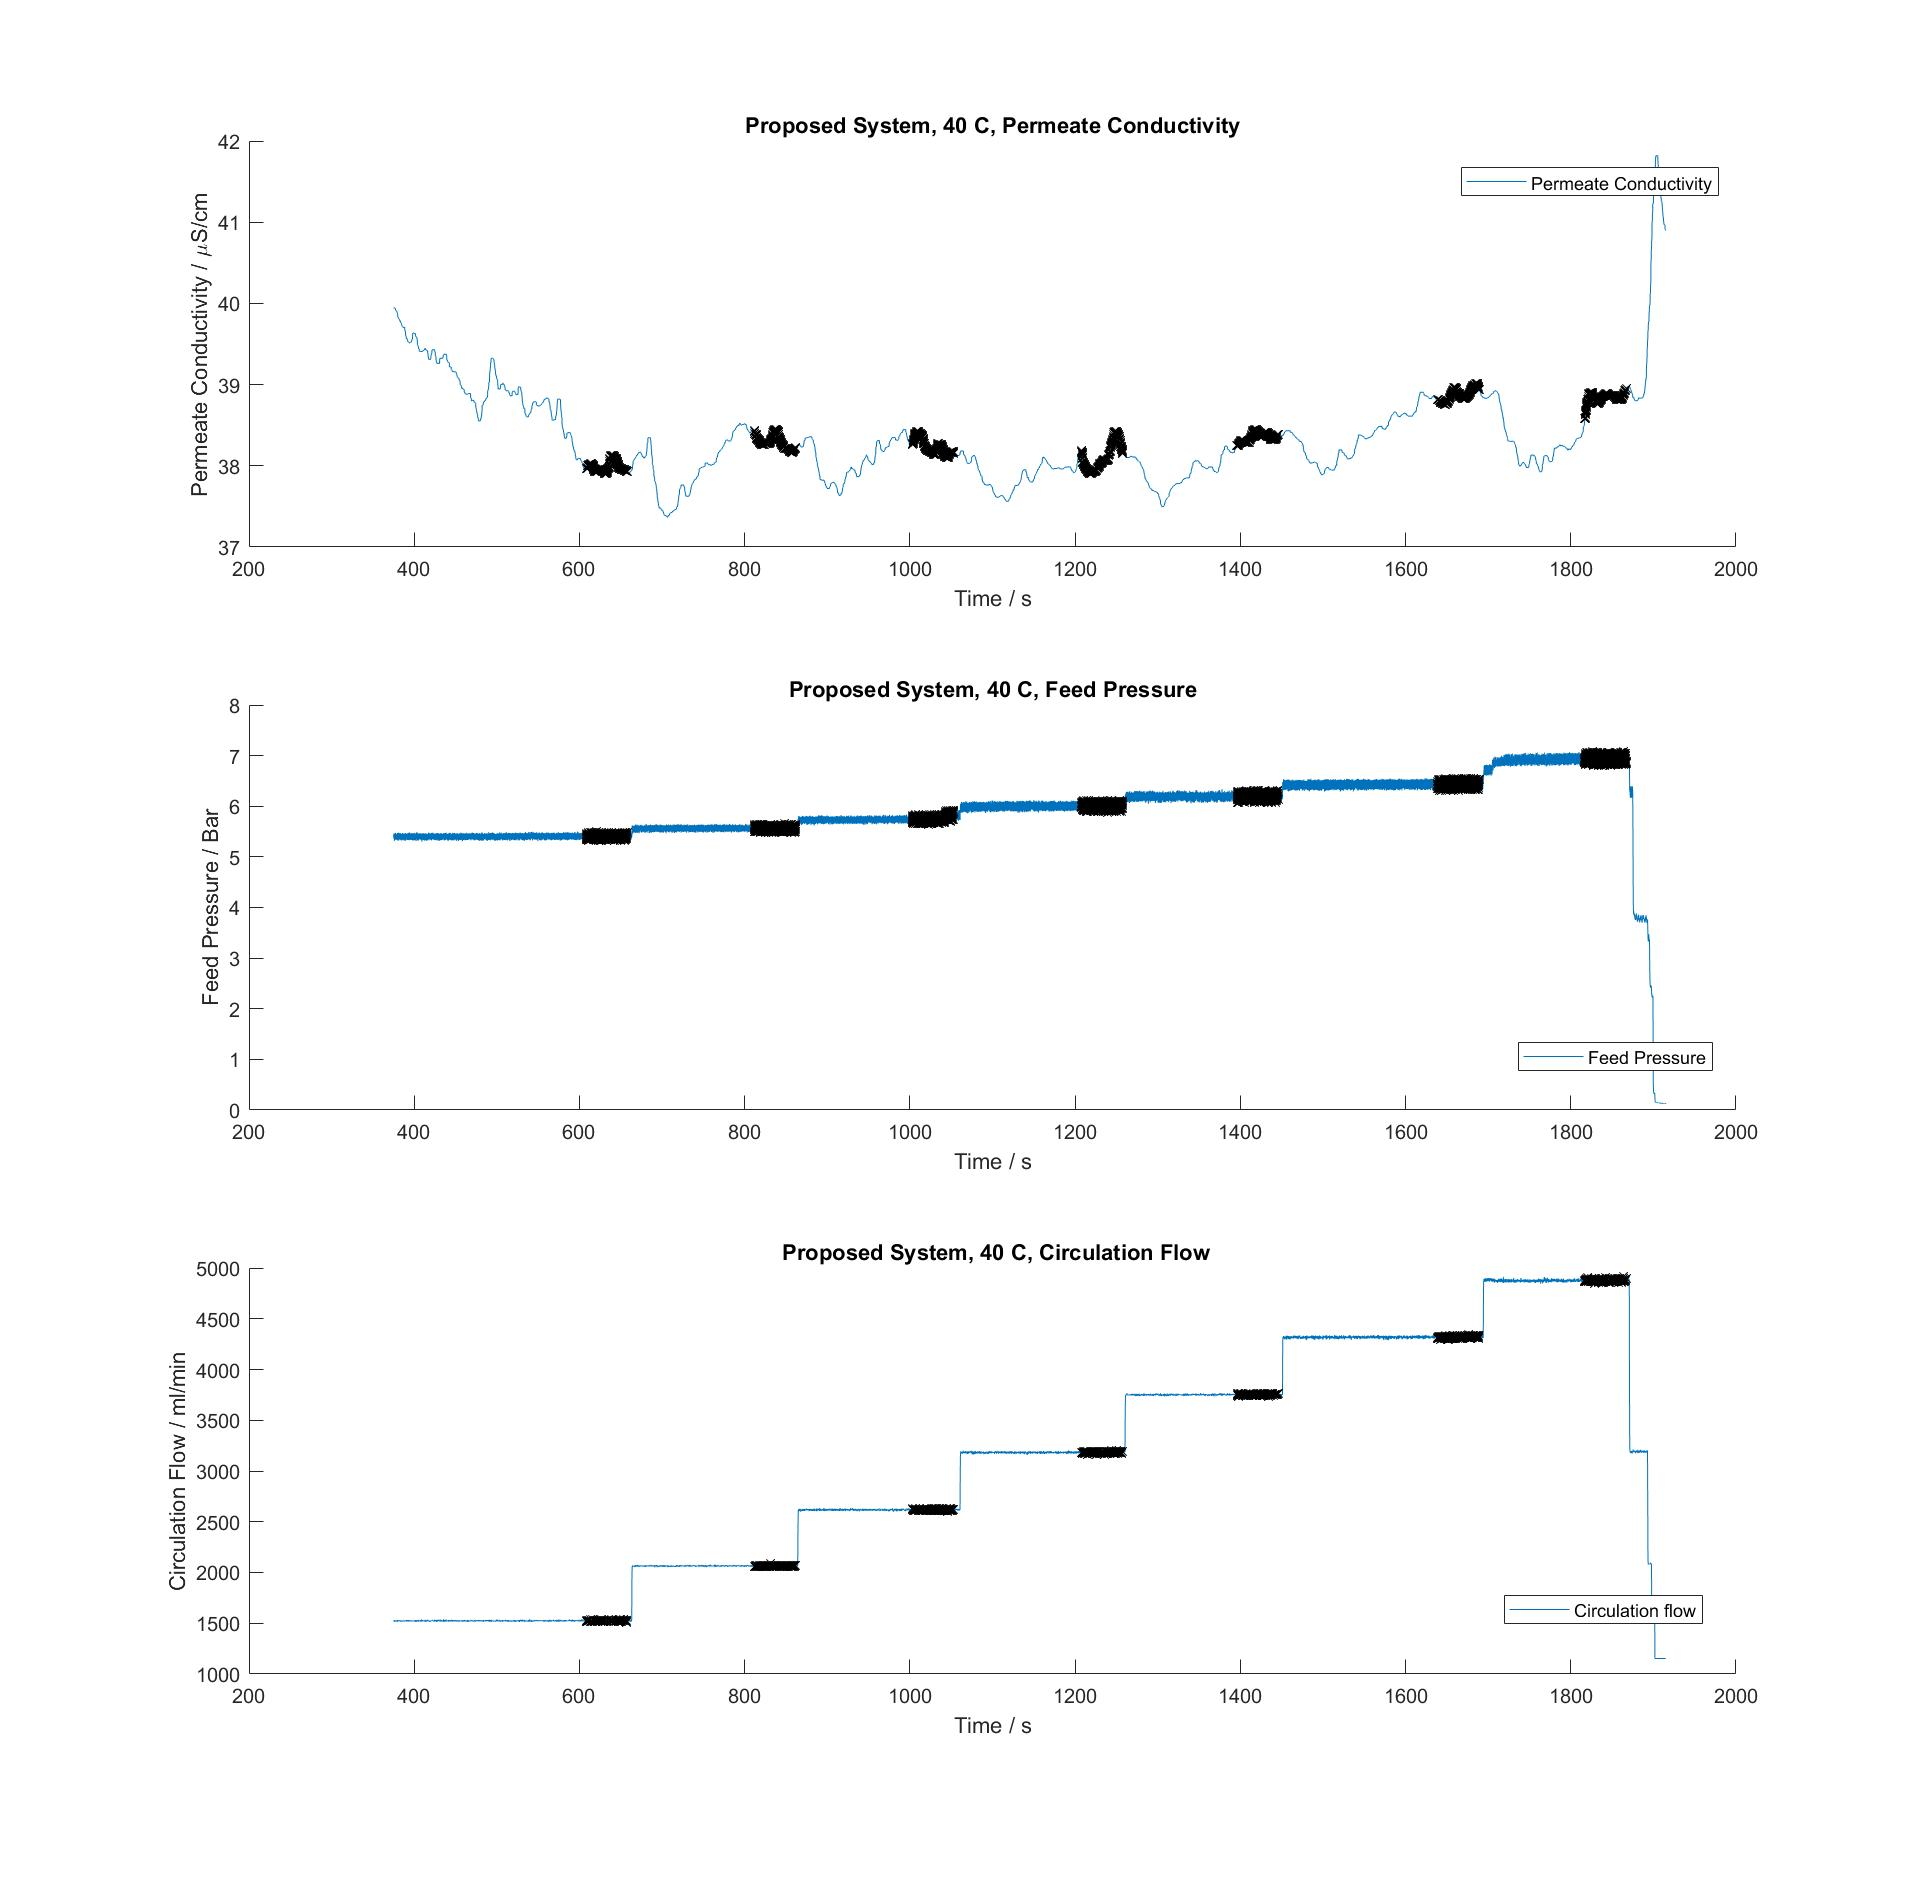
\includegraphics[width=1.1\textwidth]{RecIncrease40}
    \caption{Caption missing}
    \label{fig:RecIncrease}
\end{figure}  

More information about how the system performed during the test was calculated and can be seen in figure \ref{RecIncreaseKey}. The Recovery decreased from 22\% to 14\%  but salt rejection and permeate conductivity did only increase slightly. 
\begin{figure}[H]
    \centering
    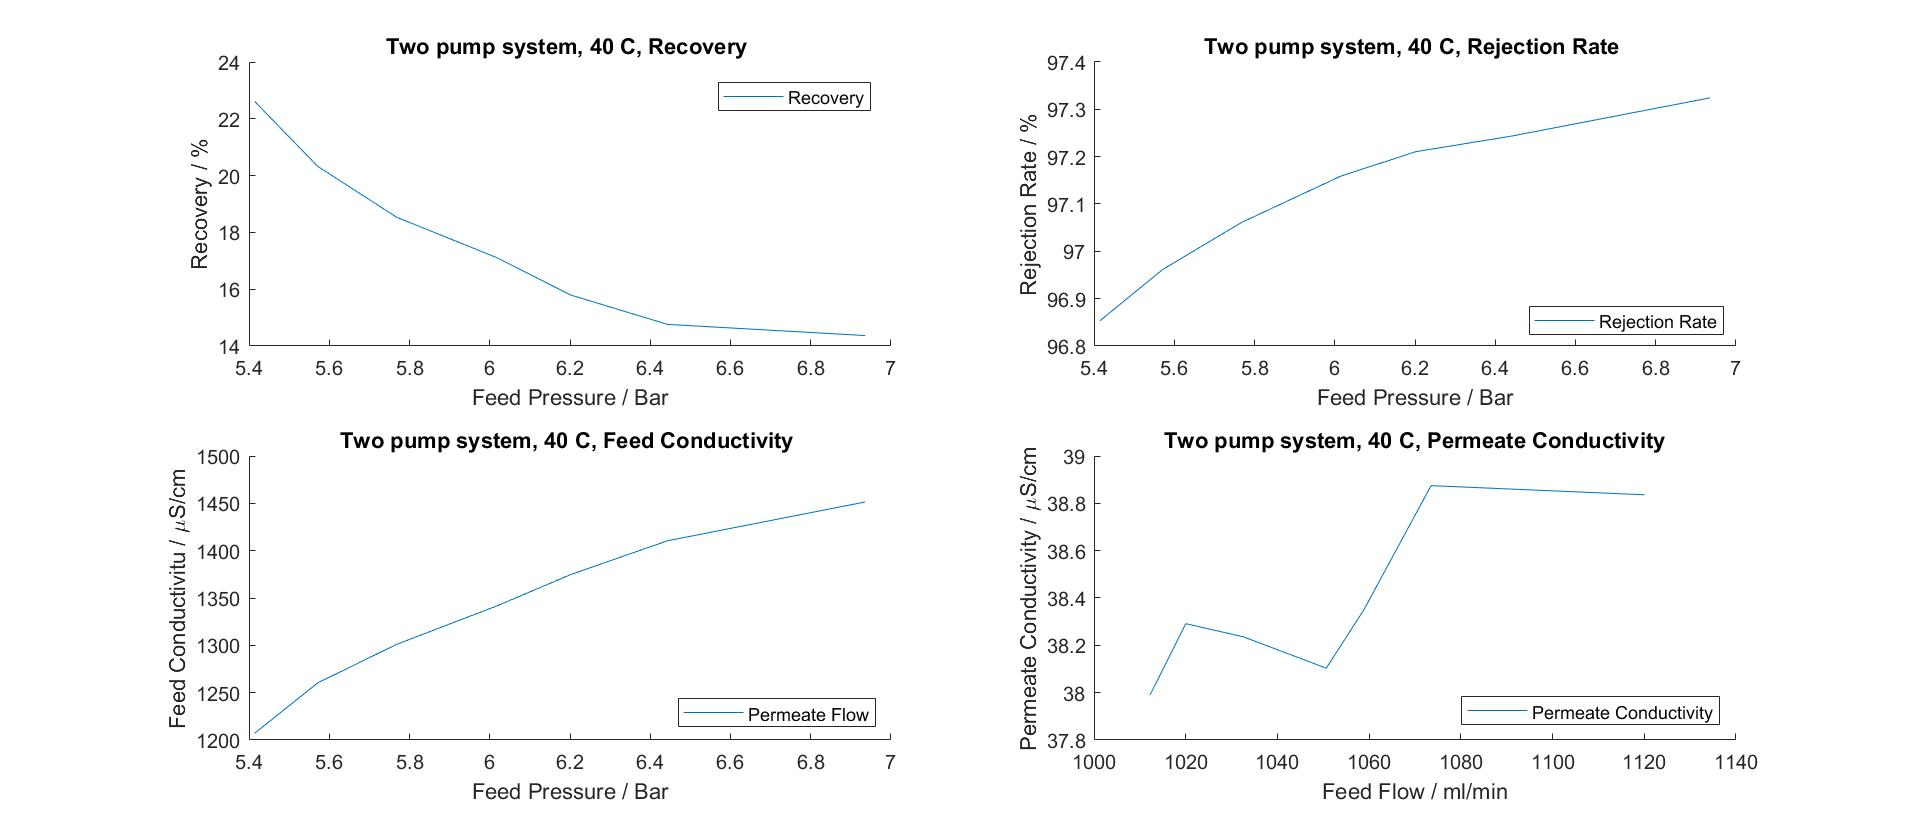
\includegraphics[width=1.1\textwidth]{RecIncrease40Key}
    \caption{Caption missing}
    \label{fig:RecIncreaseKey}
\end{figure} 
\par\bigskip 
\noindent
The test concluded that the initial theory that increased circulation flow would lead to better system performance was false. Increasing the circulation has no measureable positive effect on the system. 

\newpage
\subsubsection{increased circulation}
The next test was set up to investigate the effect of an increased feed pressure. During the test all parameters were kept constant except the rpm of the feed pump. An overview of the test can be seen in figure \ref{fig:FeedPumpIncrease40} and the key parameters calculated after the test can be seen in figure \ref{fig:FeedPumpIncrease40Key} 

\begin{figure}[H]
    \centering
    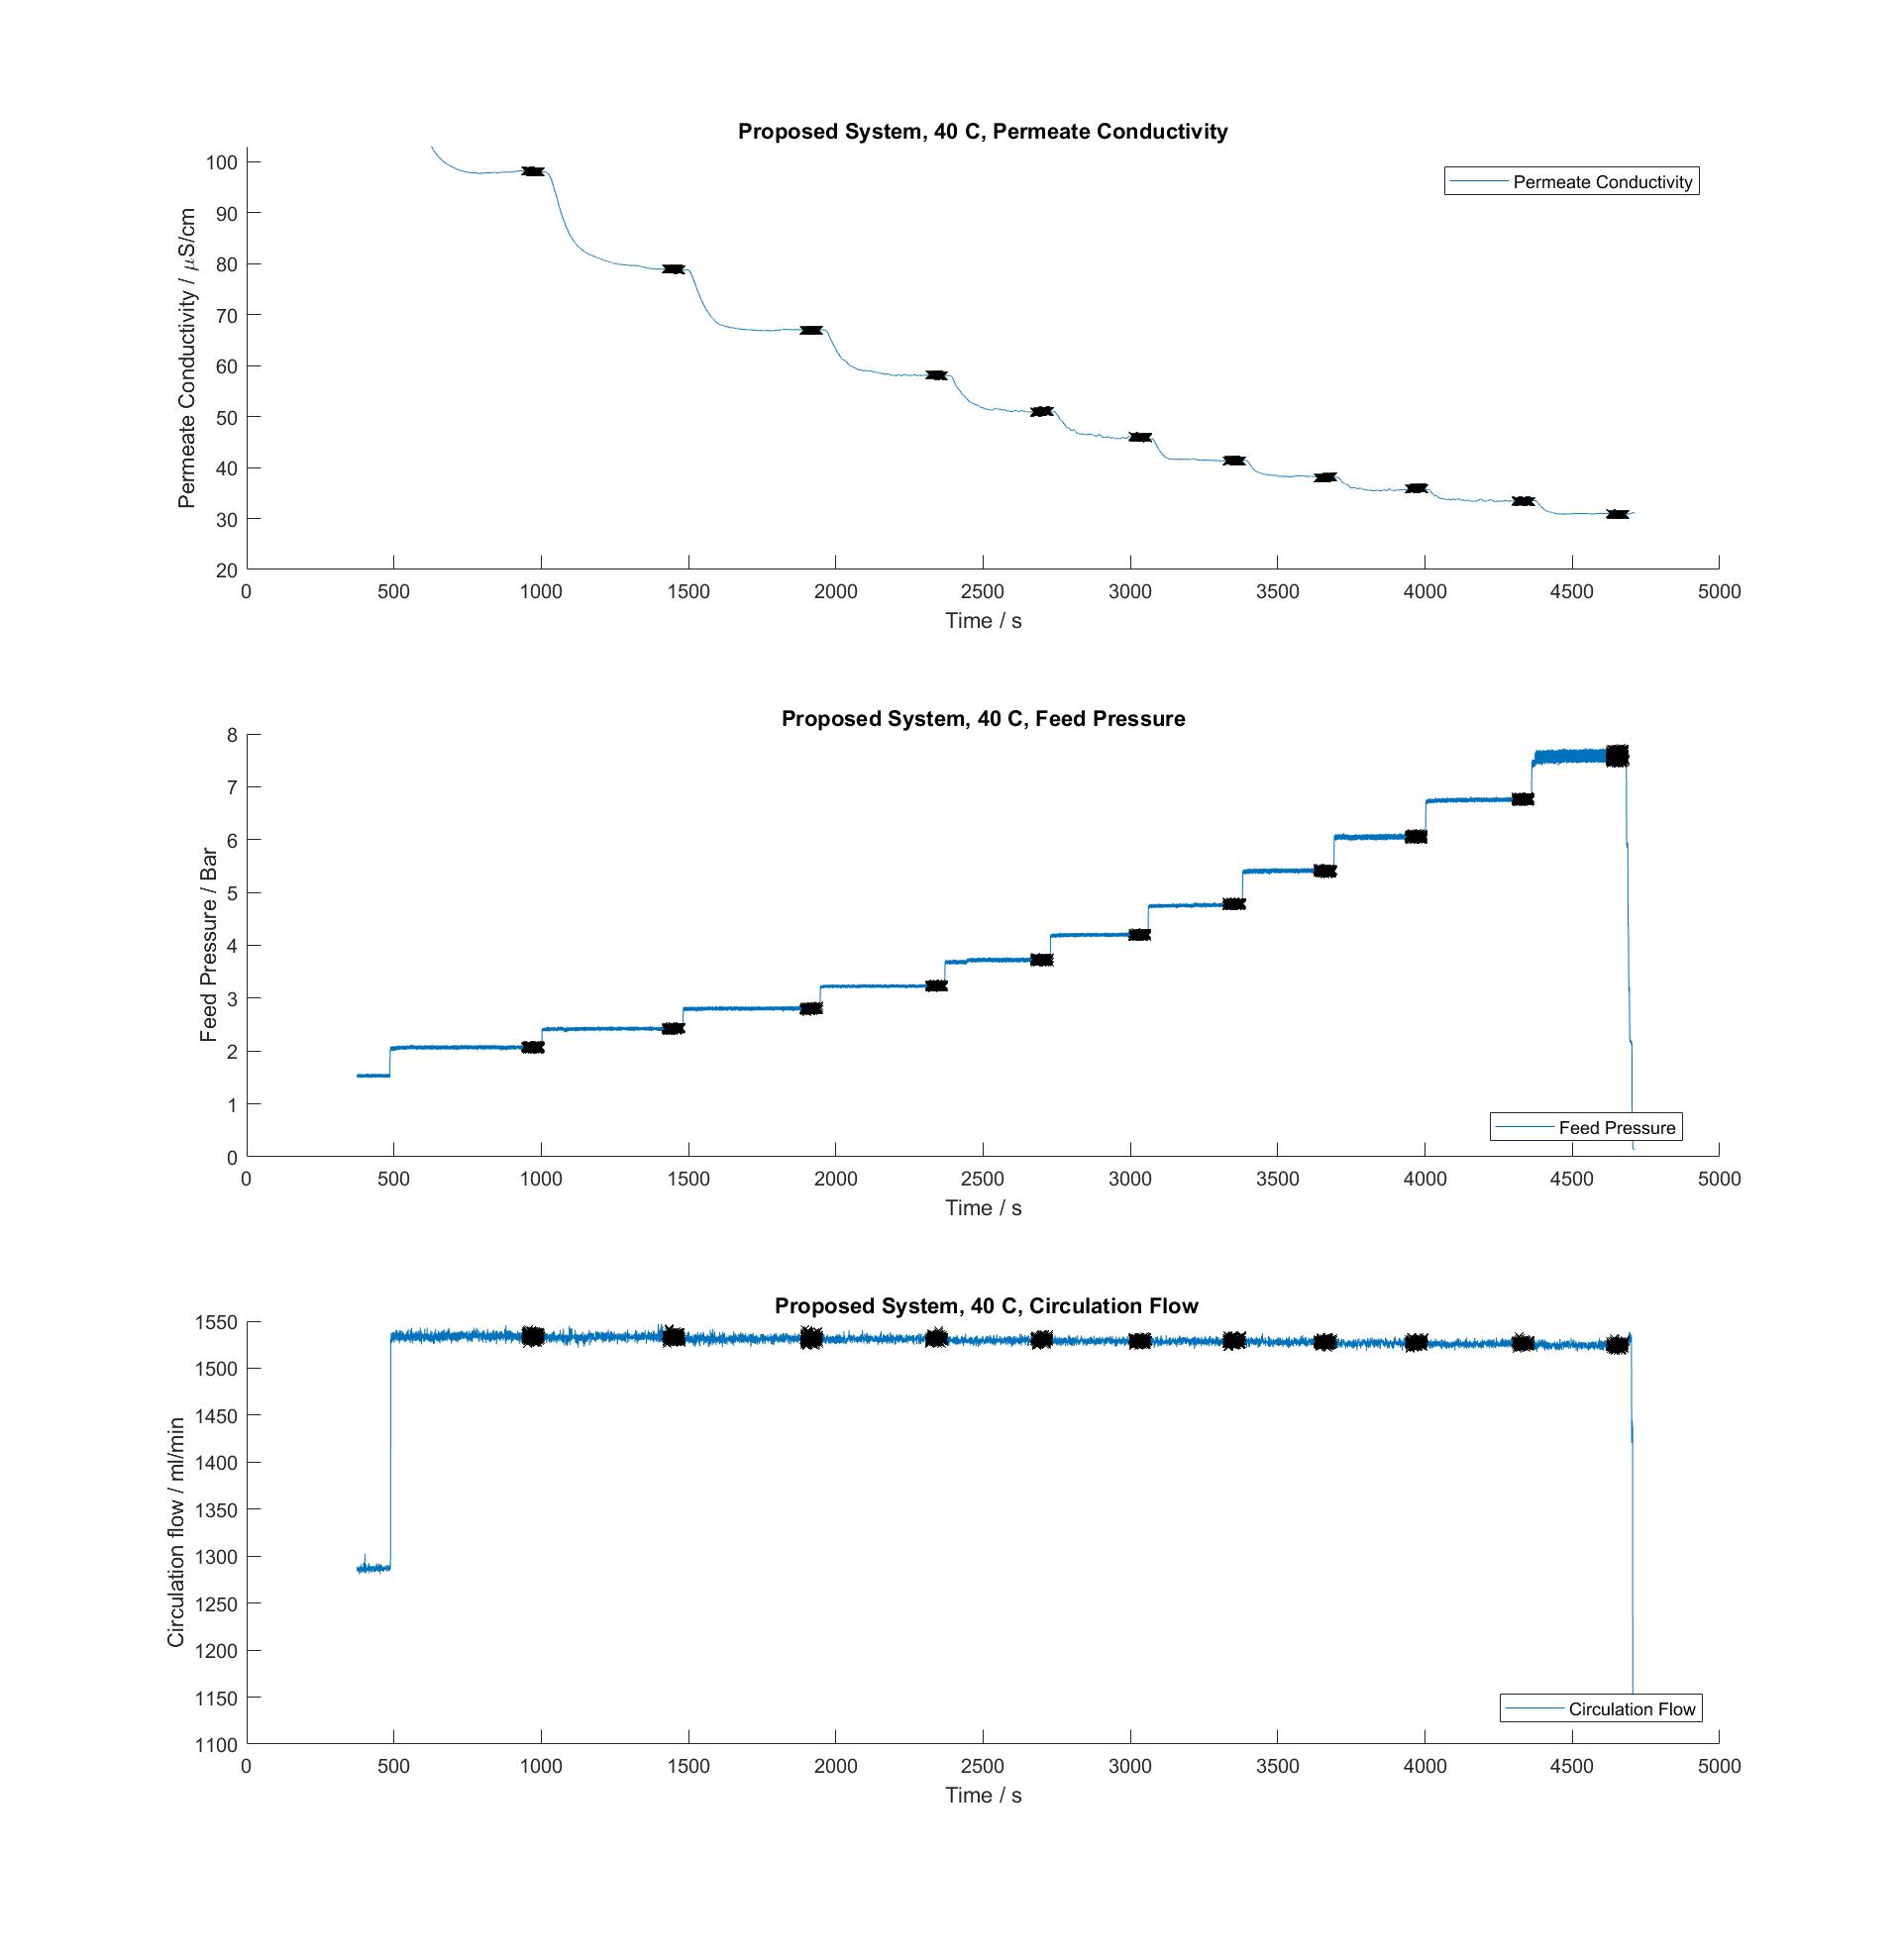
\includegraphics[width=1.1\textwidth]{FeedPumpIncrease40}
    \caption{Caption missing}
    \label{fig:FeedPumpIncrease40}
\end{figure}

\begin{figure}[H]
    \centering
    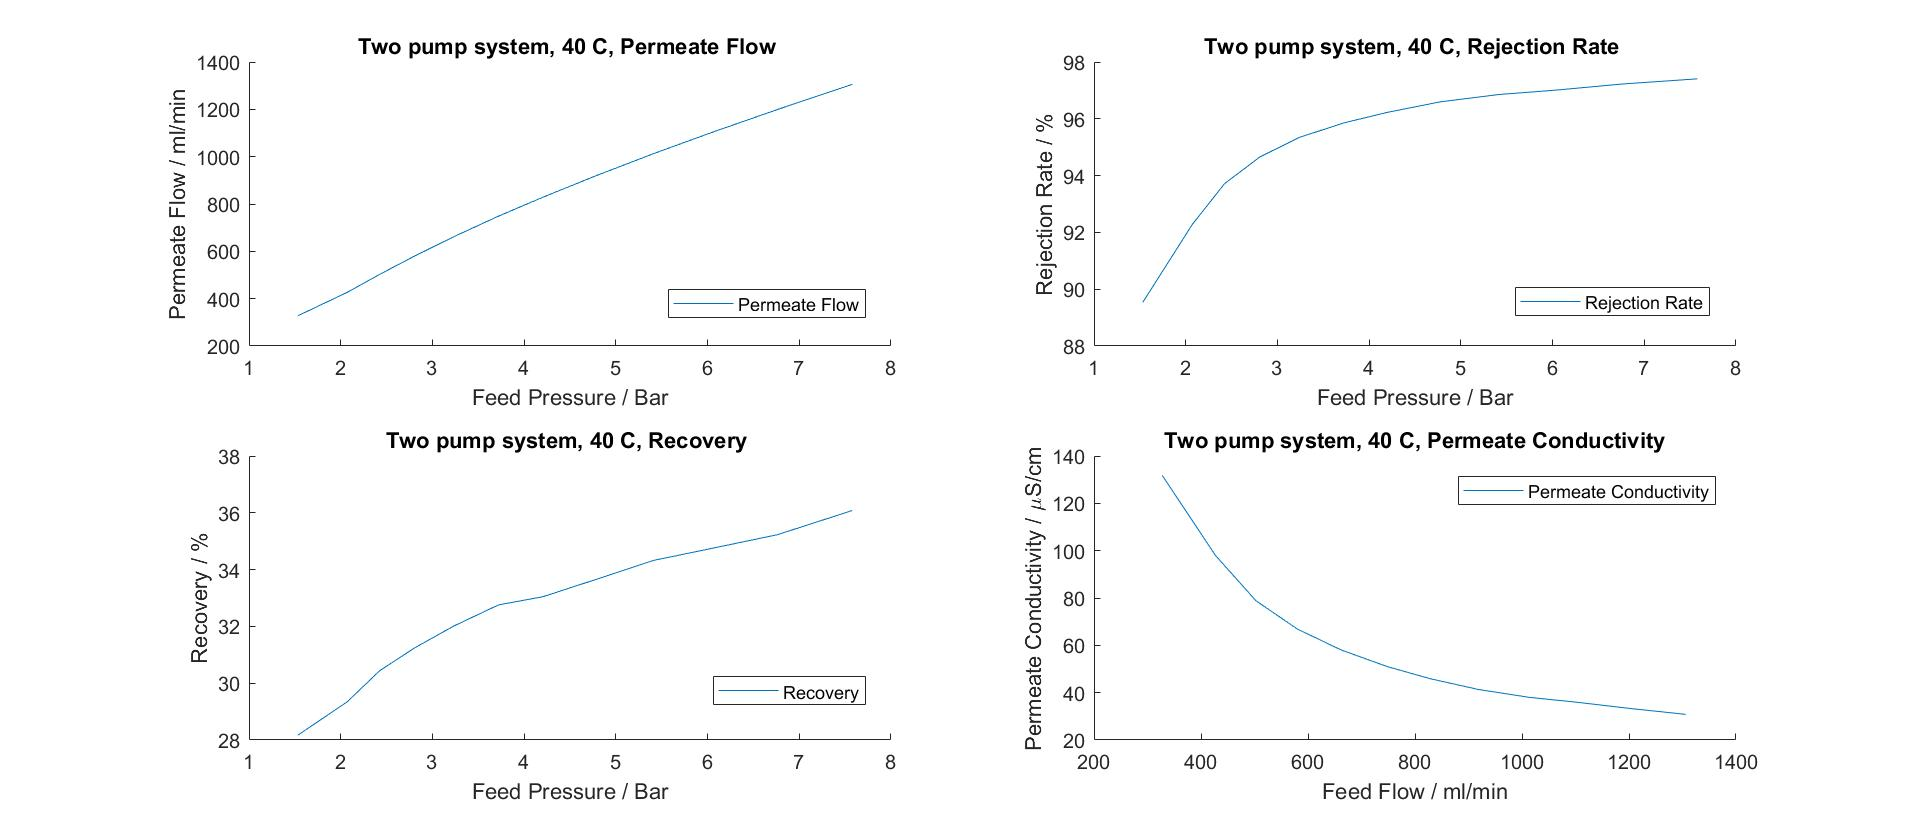
\includegraphics[width=1.1\textwidth]{FeedPumpIncrease40Key}
    \caption{Caption missing}
    \label{fig:FeedPumpIncrease40Key}
\end{figure}

From figure \ref{fig:FeedPumpIncrease40} it can be seen that the circulation flow remained constant and that the feed side pressure was increased from 1.5 to 8 bars. The permeate quality increased from 100 uS/cm to 30 uS/cm. As a result, it could be concluded that it was possbile to increase the performance of the membrane by increasing feed side pressure without the increased circulation flow. It should be noted that  the membrane recovery increased from 28\% to 36\% during the test and this is far above the maximum limit specified by the manufacturer. Therefore, it should also be concluded that only controlling the feed pump without controlling membrane recovery could damage the membrane. 

SAVING ENERGY COSTS WATER / VICE VERSA!


 
\newpage
\subsection{Optimization algorithm}

Previous tests concluded that it was ineffective to increase salt rejection by increasing the circulation flow, that it was possible to increase feed side pressure to increase salt rejection and that water temperature was the parameter that had the largest deterimental effect on salt rejection. Increased feed water conductivity also decreased the performance of the system, but not as much as increased temperature and the negative effect of high conductivity was more prominant at higher temperatures. Increased feed side pressure has a larger possitive effect on salt rejection at high temperature.
Since test showed that increased temperature decreased net driving pressure (See figure \ref{fig:NDP}) and that decreased feed pressure reduced salt rejection (see figure \ref{fig:SalrRejectionResult} it could be concluded that using a fixed value setpoint at either feed side pressure or permeate flow would not work. Instead a setpoint could be calculated for a given temperature and pressure or permeate flow could be used as a setpoint.
By using permeate flow instead of feed side pressure as a setpoint, factors such as membrane fouling, scaling and individual differences in the membrane could be compensated by the controller.

\subsection{Finding an optimal plane}

the purpose was to find a permeate flow setpoint that would ensure good quality peremeate at all temperatures without wasting more water and energy than needed. Since it was concluded in previous tests that membrane recovery did not improve saltrejection it was determined that this parameter should be set to 20\%. 

The goal of the test was to find the lowest pressure needed at a given feed conductivity and temperature to achieve a permeate conductivity of 30 uS/cm while maintaining a recovery of at most 20\%. The test was conducted by first adjusting the temperature in the heating bath to 20 deg C and then add salt so that the conductivity of the water in the bath was roughly 275 uS/cm. Afterwards, the feed and circulation pump were adjusted to obtain a  permeate conductivity of 30 uS/cm and 20\% recovery. Once the system had stabilised important parameters were noted. Once the parameters had been obtained, the conductivity was slowely increased and the pumps were modified to once again produce peremate water with a conductivity of 30 uS/cm. This procedure was repeated until the conductivity reached 3000 uS/cm. The same procedure was repeated using 30 C and 40 C inlet water.



\section{Design of control algorithms}
In order to design control for driving the system some investigations on System 2, the two pump solution were done. In picture \ref{fig:PreTestReg1}, the results from test with all parameters except the speed of the recycle pump were kept constant, can be seen. \\
\\
In picture \ref{fig:PreTestReg3}, the results from test with all parameters except the speed of the feed pump were kept constant, can be seen.

\begin{figure}[h]
    \centering
    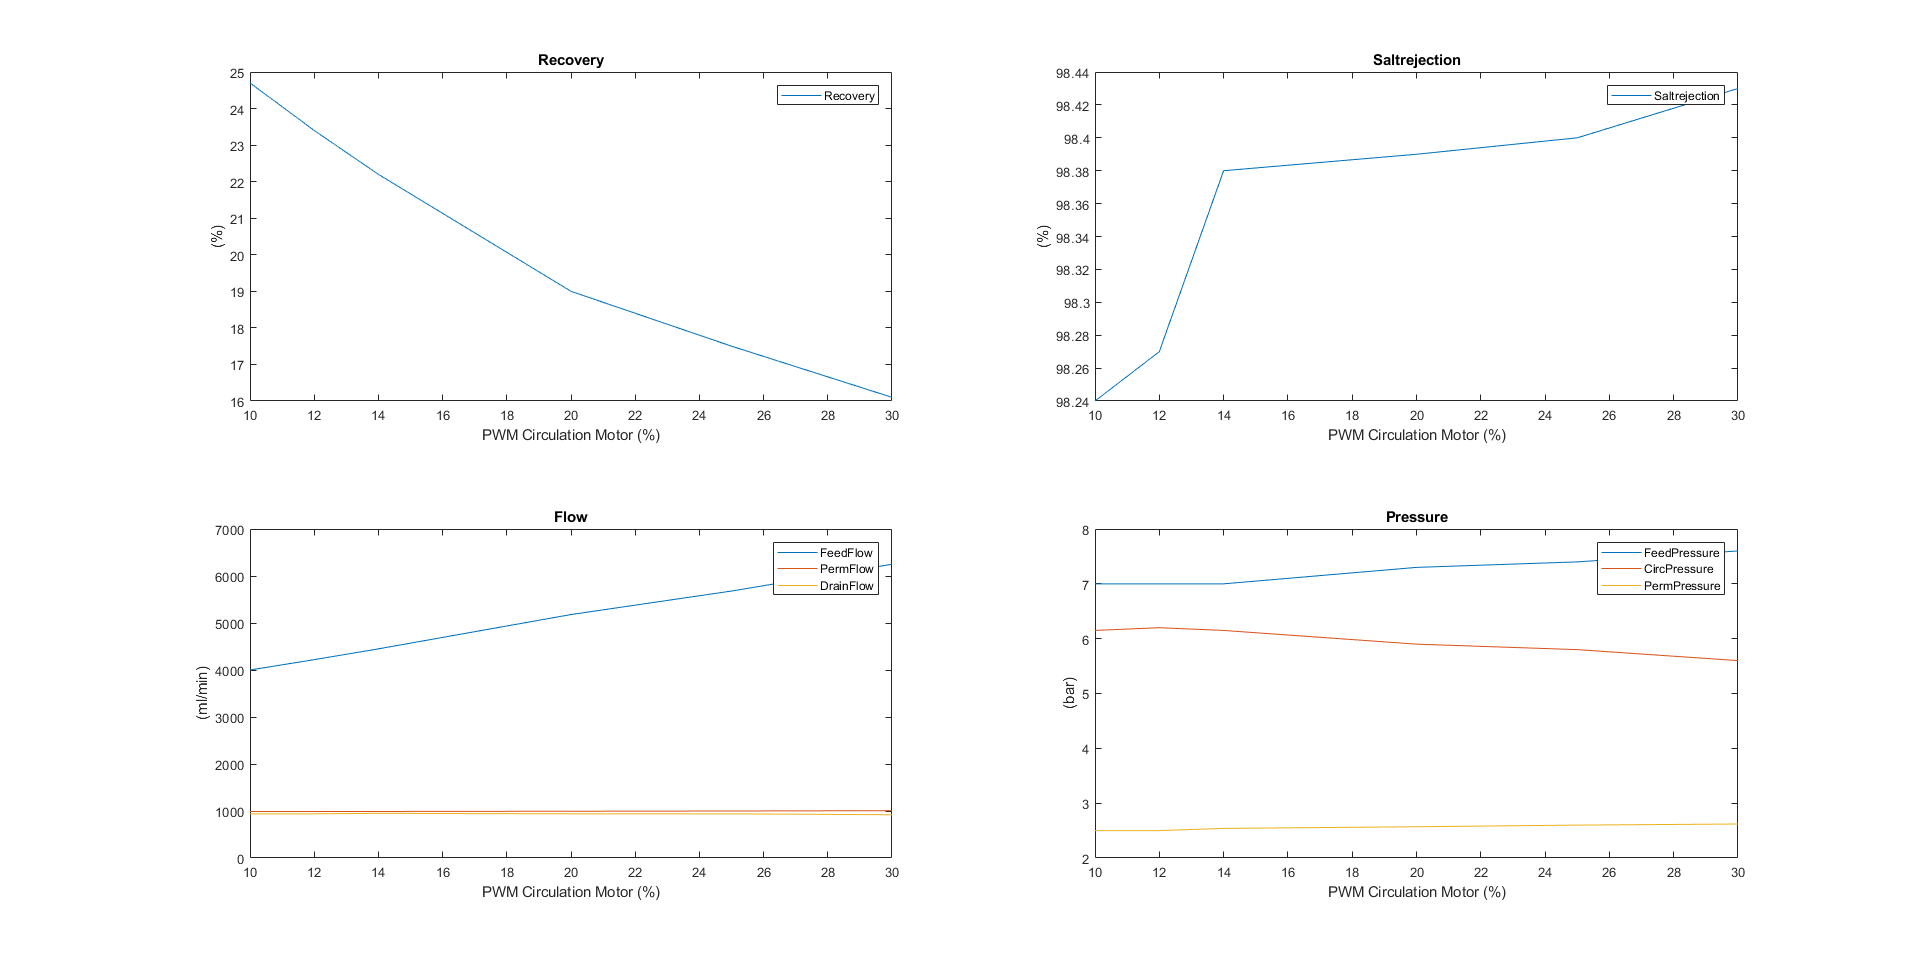
\includegraphics[width=1.65\textwidth, angle = 270]{PreTestReg1.png}
    \caption{Tests with recycle pump as changing parameter}
    \label{fig:PreTestReg1}
\end{figure}

\begin{figure}[h]
    \centering 
    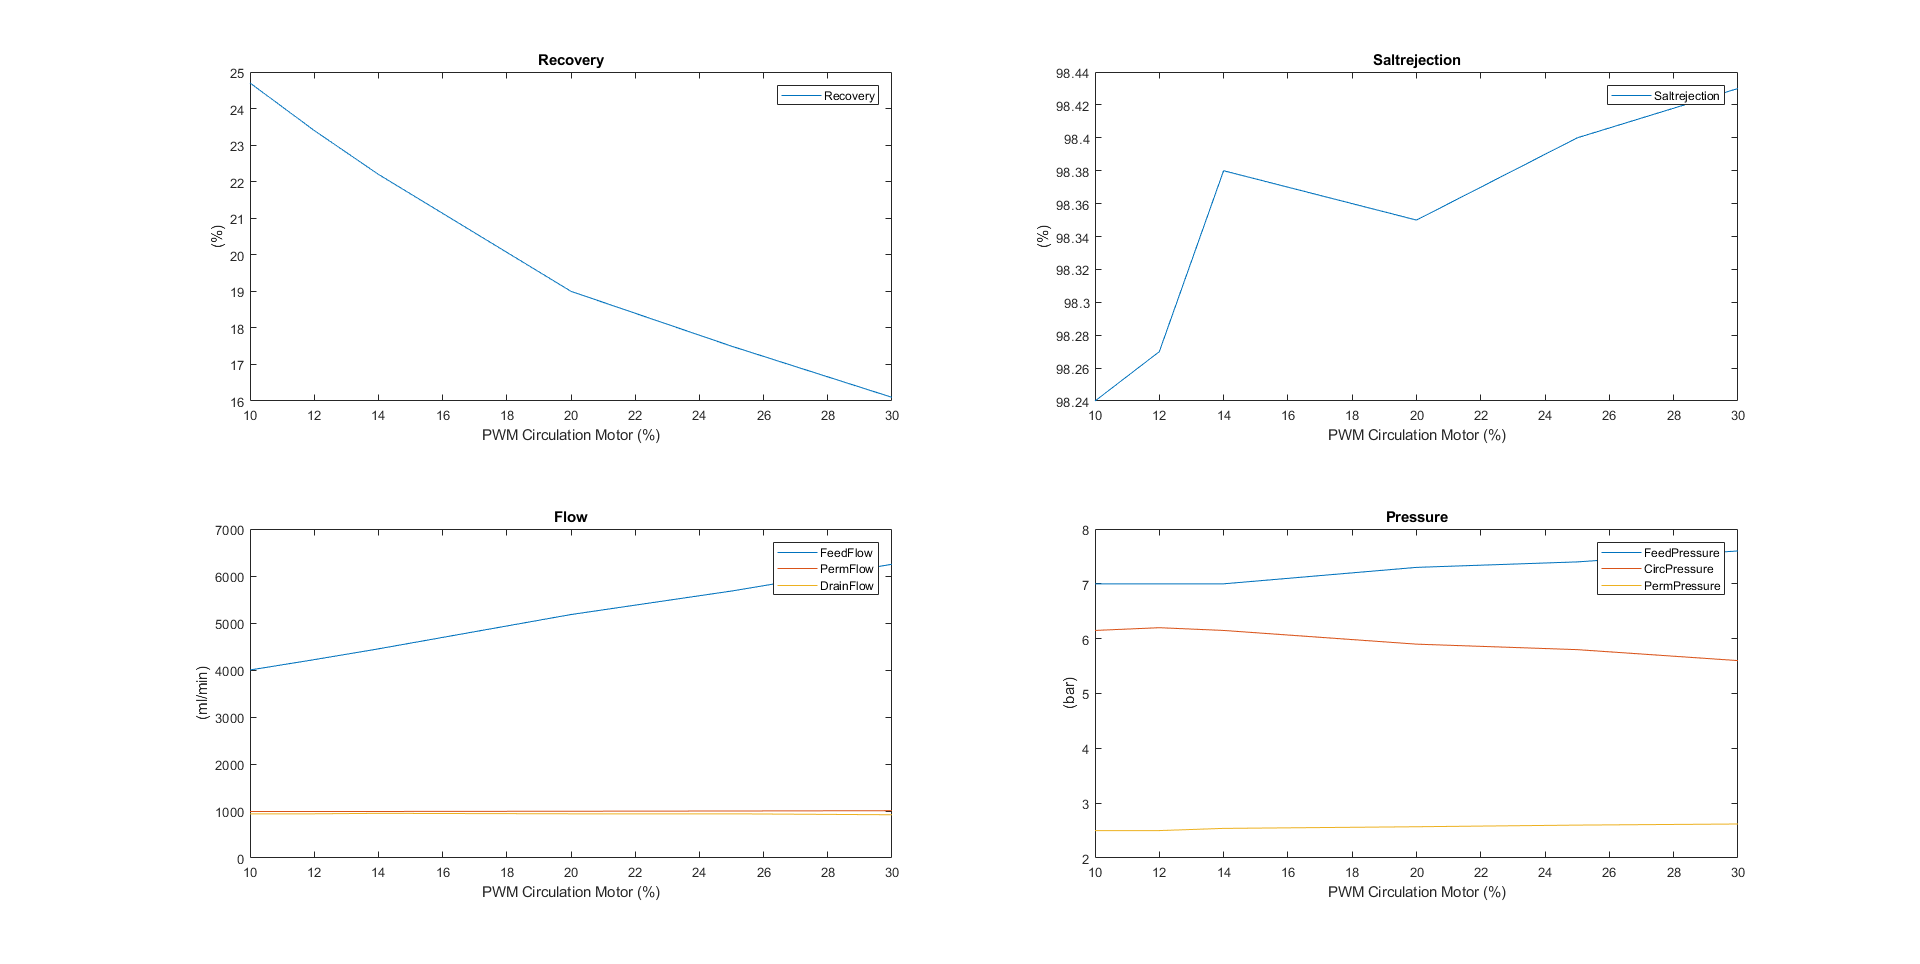
\includegraphics[width=1.65\textwidth, angle=270]{PreTestReg3.png}
    \caption{Tests with feed pump as changing parameter}
    \label{fig:PreTestReg3}
\end{figure}





